\documentclass{mldsmsc}
% \setlength{\parindent}{20pt}

\title{Probabilistic Sequential Matrix Factorisation for 12-Lead \\ ECG Data}
\author{Joana Levtcheva}
\CID{01252821}
\supervisor{Dr Deniz Akyildiz}
% \date{1 May 2023}
%For today's date, use:
\date{\today}
\logoimg{}


% THIS IS WHERE NEW COMMANDS CAN BE DEFINED
% commands below only used in the proof; otherwise can be deleted
\newcommand{\consta}{a}
\newcommand{\X}{X}
\newcommand{\EE}[1]{ \mathrm{E} [ #1 ] }
\newcommand{\inparenth}[1]{\left( #1 \right)}

\begin{document}

% Generates the Title Page
\maketitle


% Generates plagiarism declaration
\declarationname{Joana Levtcheva}
\declarationdate{\today}
\declaration 

\begin{abstract}

Matrix factorisation (MF) techniques are highly effective and widely used in unsupervised machine learning. By decomposing the original matrix into multiple simpler lower-dimensional matrices, MF aims to uncover latent structures that are not immediately obvious in the original matrix. MF finds applications in areas such as image processing, natural language processing, missing data imputation, and recommendation systems. Despite considerable progression in the probabilistic versions, there is demand for such methods in applications such as uncertainty quantification, managing time-series data, and executing efficient probabilistic computations. \newline

\noindent In this thesis, we show novel applications of the probabilistic sequential MF algorithm Probabilistic Sequential Matrix Factorisation (PSMF) (\cite{akyildiz2021probabilistic}) to 12-lead ECG data. We explore three tasks related to this complex high-dimensional time-series data with nonlinear subspace: missing data imputation with PSMF and the robust version of PSMF (rPSMF) (\cite{akyildiz2021probabilistic}) and compare their performance with other probabilistic sequential MF algorithms, R-peaks detection, and forecasting an ECG component based on previous normal heart beats using a Fourier basis with multiple terms and rank higher than one. We perform our experiments using the high-quality comprehensive dataset "A Large Scale 12-lead Electrocardiogram Database for Arrhythmia Study" (\cite{cite1}, \cite{cite2}, \cite{cite3}). We describe and outline the experimenting process and the challenges we encountered modelling the complex ECG data, and summarise the experiments results. We find that PSMF performs well when used for imputing missing data, but when it comes to forecasting there are certain challenges which open the door for further research on extending the PSMF algorithm to better handle the complex structure of ECG data. \newline

\end{abstract}

\begin{acknowledgements}

TODO 

\end{acknowledgements}

% add glossary?

% table of contents
\tableofcontents

% VERY IMPORTANT
% This command switches from Roman to Arabic numbering for main part of thesis
\mainmatter


\chapter{Introduction}

Matrix factorisation (or also matrix decomposition) in the context of linear algebra is simply a factorisation of a matrix into a product of multiple matrices. Many different decompositions exist, and they find various applications in mathematical problems such as solving systems of linear equations, matrix inversion, determinant computation, eigenvalues problems, solving systems of first order ODEs, etc. \newline

\noindent In this thesis, we are interested in matrix factorisation (MF) in the context of machine learning. Nowadays, MF techniques are highly effective and widely used in unsupervised machine learning. These methods aim to decompose the original matrix into multiple lower-dimensional matrices. By breaking the matrix into these simpler components MF aims to uncover latent structures that are not immediately apparent in the original matrix. Some applications are in image processing: for reducing dimensionality and noise in images, NLP for topic modelling, missing data imputation, recommendation systems, etc. \newline

\noindent Formally, we are interested in the general problem of factorising a data matrix $Y \in \mathbb{R}^{m \times n}$ as

\begin{equation}
Y \approx CX,
\end{equation} \newline
\noindent where $C \in \mathbb{R}^{m \times r}$ is the \textit{dictionary matrix}, $X \in \mathbb{R}^{r \times n}$ is the \textit{coefficients matrix} (with columns the coefficients), and $r$ is the \textit{approximation rank} (\cite{cite-key}). Visually we can present the problem as

\begin{equation}
\underbrace{
\begin{bmatrix}
  \times & \times & \times & \times & \times \\
  \times & \times & \times & \times & \times \\
  \times & \times & \times & \times & \times
\end{bmatrix}
}_{\text{Y $\in \mathbb{R}^{m \times n}$ }}
\approx
\underbrace{
\begin{bmatrix}
  \times & \times \\
  \times & \times \\
  \times & \times
\end{bmatrix}
}_{\text{C $\in \mathbb{R}^{m \times r}$ }}
\underbrace{
\begin{bmatrix}
  \times & \times & \times & \times & \times \\
  \times & \times & \times & \times & \times
\end{bmatrix}
}_{\text{X $\in \mathbb{R}^{r \times n}$ }}.
\end{equation}

\noindent There are also probabilistic versions of MF which incorporate probabilistic models to better handle uncertainty and variability in the data, leading to more accurate predictions. Such methodologies postulate a prior distribution over the latent factors and necessitate the computation of the posterior distribution to derive updated estimates. With that the matrix is not only decomposed but probabilistic interpretations of the factors are also possible. \newline

\noindent We should also note that some algorithms are suitable for sequential data - updating $C$ and $X$ incrementally as new data points are observed and thus incorporating temporal dynamics and sequential dependencies into the factorisation process, and others are non-sequential - treating the dataset as a batch, independent of the time varying component. \newline

\noindent Throughout this thesis we are going to focus on probabilistic sequential MF algorithms, along with their application to 12-lead ECG data, targeting the problem of managing high-dimensional time-series data with nonlinear subspace. Some examples of probabilistic MF algorithms are Probabilistic Matrix Factorisation (PMF) (\cite{NIPS2007_d7322ed7}) - non-sequential, Dictionary filtering (\cite{cite-key}), Probabilistic Sequential Matrix Factorization (PSMF) (\cite{akyildiz2021probabilistic}). \newline

\noindent The paper "Probabilistic matrix factorisation" (PMF) (\cite{NIPS2007_d7322ed7}) introduces an efficient and scalable probabilistic model for collaborative filtering. The algorithm performs well on large, sparse and imbalanced datasets. This is demonstrated by using a Netflix dataset, where PMF models the user preference matrix $R$ as a product of two lower-dimensional matrices: user feature matrix $U$ and movie feature matrix $V$. The conditional distribution over observed ratings is modeled using Gaussian noise, and zero-mean spherical Gaussian priors are placed on the user and movie feature vectors. The paper also presents two extensions to the initial PMF model: incorporating \textit{adaptive priors} to automatically control the model complexity through these priors over the model parameters, and a \textit{constrained PMF} version to handle and improve predictions for users with few ratings by incorporating constraints based on the assumption that users with similar movie ratings have similar preferences. The authors show that PMF significantly outperforms traditional Singular Value Decomposition (SVD) (\cite{4ba978eb-d878-342d-a11e-6d7554474b2d}) models and scales linearly with the number of observations. It's worth noting that PMF treats each rating as an independent event meaning the time varying component is not taken into consideration, making PMF a batch learning model designed to process large datasets in a non-sequential manner. \newline

\noindent Later, in the paper "Dictionary Filtering: A Probabilistic Approach to Online Matrix Factorization" (DF) (\cite{cite-key}), the authors introduce a novel online MF algorithm known as dictionary filtering. It leverages probabilistic models, specifically using recursive linear filters, and efficiently factorises the original data matrix into a dictionary matrix and a coefficients matrix. This is an online and sequential algorithm, meaning it is suitable for high-dimensional and time-varying data, and it also has easy to tune parameters. DF is efficient for high-dimensional data with its computational complexity of $O(mr^2)$ independent of the number of data points. Although the model can learn non-stationary and dynamic data, it is developed for linear and Gaussian state space models (SSM). Particularly for ECG data, ECG has a nonlinear SSM which doesn't suit the dictionary filtering. \newline

\noindent Two years later, Akyildiz et.al. develop Probabilistic Sequential Matrix Factorization (PSMF) (\cite{akyildiz2021probabilistic}). This method is tailored to time-varying and non-stationary datasets consisting of high-dimensional time-series. Nonlinear Gaussian SSMs are considered, decomposing the original matrix into a dictionary matrix and time-variying coefficient matrix. This time, the matrices are with potentially nonlinear dependencies, with PSMF efficiently capturing temporal dependencies through Markovian structures on the coefficients, making it possible to encode the dependencies into a lower dimensional latent space. The model is demonstrated to work on tasks such as forecasting, changepoint detection, missing data imputation, and is shown to work on real-world data with a periodic subspace. There is also a robust version rPSMF using Student-t filters to handle model misspecification, and a version for imputing missing data. Although the model is suitbale for reducing high-dimensional data with periodic subspaces to lower-dimensional latent space, PSMF might struggle with very large datasets, having many data points. \newline

% \noindent In the unpublished MSc thesis (Imperial College London) of Rina Maletta (\cite{rina}), the author introduces Matrix-Variate Gaussian Matrix Factorization (MVGMF). This is a novel PMF method using matrix-variate Gaussian distributions. The algorithm has fast Gaussian updates which take the form of a preconditioned MF algorithm which is stable. An extension for handling missing data and data imputation is also proposed. The method is tested on the Netflix Prize dataset, London air quality (NO2) data, and Olivetti face image dataset.

\section{Contributions}

Using probabilistic methods, and specifically probabilistic sequential MF ones, on ECG data is not widely explored. Hence, we aim to introduce a few novel real-world applications of the PSMF method to 12-lead ECG data. The contributions made in this thesis are:

\begin{itemize}
    \item We show three novel applications of PSMF to complex 12-lead ECG data.
    \item Application 1: We apply both PSMF and rPSMF for imputing missing data in the ECG signals, and compare the results with other sequential probabilistic MF models.
    \item Application 2: We show that PSMF can be used for R-peaks detection by introducing a simple approach. We remove the reconstructed signal, which has modelled the R-peaks smoother than the real ones, from the original data, and determine a suitable threshold for selecting the peaks. 
    \item Application 3: We forecast an ECG component based on previous normal heart beats by incorporating a Fourier basis with multiple Fourier terms and rank higher than 1. 
    % We experiment with the original high quality data with many points, as well as with a subsample of the data, defining the ECG signals with lower frequency. We also experiment with smoothing the data, standardising it and/or normalising it. We make conclusions based on the done analysis and comparison of performance and results.
\end{itemize}

\section{Notation}

We are going to denote the original data matrix as $Y \in \mathbb{R}^{m \times n}$, and let $y_k$ denote the $k$-th column of the matrix. Also, let $y = \text{vec}(Y) \in \mathbb{R}^{nm}$ be the vectorization of the matrix $Y$:

\begin{equation}
    y := vec(Y) = \begin{bmatrix}
        y_1 \\
        y_2 \\
        \vdots \\
        y_n, 
    \end{bmatrix}
\end{equation}

\noindent where $y_1, ..., y_n$ are the columns of $Y$. The inverse is denoted as $Y := \text{vec}^{-1}(Y, m, n)$, where $m$, and $n$ specify the size of the resulting matrix. With $y_{1:k} = \{y_1, ..., y_k\}$ we are going to denote sequences. Further, let $C \in \mathbb{R}^{m \times r}$ be the dictionary matrix, $X \in \mathbb{R}^{r \times n}$ be the coefficients matrix, and $r$ be the approximation rank. \newline

\noindent With $I_d \in \mathbb{R}^{d \times d}$ we are going to denote the identity matrix, with $\mathcal{N}(x; \mu, \Sigma)$ the multivariate normal distribution with mean $\mu$ and $\Sigma$ the covariance matrix, with $\mathcal{MN}(X; M, U, V)$ the matrix normal distribution with $M$ the mean-matrix, $U$ the row-covariance, and $V$ the column covariance, with  $\mathcal{IG}(s; \alpha, \beta)$ the inverse gamma distribution with shape $\alpha$ and scale $\beta$, and finally with $\mathcal{T}(x; \mu, \Sigma, \lambda)$ the multivariate $t$ distribution, where $\mu$ is the mean, $\Sigma$ the scale matrix, and $\lambda$ is the degrees of freedom. \newline


% \noindent  We denote the vectorised forms of the matrices with their respective lower case letters. We can formally define c = vec(C), where vec(·) is the vectorisation operation. The columns of C are stacked on each other, so if C ∈ Rm×r, then c ∈ Rmr×1. We can also define the inverse vectorisation operator C = vec−1(c). \newline

% \noindent We have that p(x) denotes the probability density function (pdf) of x and p(y|x) is the conditional density of y given x. Where A ∈ Rm×n is a matrix, then MN(A;M,U, V ) denotes the matrix normal pdf for A, where M ∈ Rm×n is the mean, U ∈ Rn×n is the among-row co-variance and V ∈ Rm×m is the among-column co-variance. We also define the multivariate normal distribution in the following way; let a ∈ Rm, then N(a; μ, Σ) denotes the pdf of the multivariate normal distribution for the random variable a, where μ ∈ Rm is the mean and Σ ∈ Rm×m is the covariance matrix. Im ∈ Rm×m is the m×m identity matrix. \newline

\chapter{Background}

\section{Preliminaries}

Here, we are going to introduce the matrix normal distribution, Kronecker product, and outline certain linear algebra properties in relation to Kronecker products. These properties are later used in some of the proofs.

\subsection{Matrix Normal Distribution}

We start with introducing the matrix normal distribution, which we are going to mainly use in its vectorised version.

\begin{definition} \label{def:mvn}
    Let $X \in \mathbb{R}^{p \times n}$ be a random matrix. Then $X$ has a $\textit{matrix normal distribution}$ $\mathcal{MN}(X; M, U, V)$ with mean-matrix $M \in \mathbb{R}^{p \times n}$, row-covariance $U \in \mathbb{R}^{p \times p}$, and column-covariance $V \in \mathbb{R}^{n \times n}$, if $\text{vec}(X) \sim \mathcal{N}(\text{vec}(M), U \otimes V)$.
\end{definition}

\noindent We can formally write that if $X \sim \mathcal{MN}(X; M, U, V)$, then 
\begin{equation} \label{eq:mndvec}
    x \sim \mathcal{N}(x; \text{vec}(M), U \otimes V),
\end{equation}

\noindent where $x = \text{vec}(X) \in \mathbb{R}^{pn}$, $\text{vec}(M) \in \mathbb{R}^{pn}$ is the mean, $U \times V \in \mathbb{R}^{pn \times pn}$ is the covariance matrix, and $\otimes$ is the Kronecker product (\cite{gupta}). \newline

\noindent Further, for the random matrix $X \in \mathbb{R}^{p \times n}$ the probability density function (p.d.f.) of the matrix normal distribution is defined as (\cite{gupta})

\begin{equation}
    (2\pi)^{-\frac{1}{2}np} |U|^{-\frac{1}{2}n} |V|^{-\frac{1}{2}p} \exp{\{-\frac{1}{2}\text{tr}(U^{-1}(X - M)V^{-1}(X - M)^{T})\}},
\end{equation}

\noindent where $|U|$ and $|V|$ are the determinants of $U$ and $V$ respectively, $\text{tr}(.)$ denotes the $\textit{trace}$ of a matrix, $X \in \mathbb{R}^{p \times n}$, $M \in \mathbb{R}^{p \times n}$.

\subsection{Kronecker Product}

Now, let's introduce the Kronecker product we already mentioned in relation to Definition \ref{def:mvn}.

\begin{definition}
Let $A \in \mathbb{R}^{m \times n}$ and $B \in \mathbb{R}^{p \times q}$ be matrices. Then their \textit{Kronecker product} denoted as $A \otimes B \in \mathbb{R}^{mp \times nq}$ is given by (\cite{alma993596394401591}):

\begin{equation}
    A \otimes B = \begin{bmatrix}
        a_{11}B & a_{12}B & \hdots & a_{1n}B \\
        a_{21}B & a_{22}B & \hdots & a_{2n}B \\
        \vdots & \vdots & \ddots & \vdots \\
        a_{m1}B & a_{m2}B & \hdots & a_{mn}B
    \end{bmatrix},
\end{equation}
where $\{a_{ij}\}$, $i \in \{1,...,m\}$, $j \in \{1, ..., n\}$ are the elements of $A$.
\end{definition}

\noindent We are also going to need certain Kronecker product related properties. If we let $A \in \mathbb{R}^{m \times n}$, $X \in \mathbb{R}^{n \times p}$, and $B \in \mathbb{R}^{p \times q}$, then (\cite{alma993596394401591})
\begin{equation} \label{eq:vecms}
    \text{vec}(AXB) = (B^T \otimes A) \text{vec}(X). 
\end{equation}

\noindent Now, if we let $x \in \mathbb{R}^n$, from Equation \ref{eq:vecms} we can obtain
\begin{equation}
    Ax = \text{vec}(Ax) = (x^T \otimes I_n)\text{vec}(A),
\end{equation}

\noindent where $I_n \in \mathbb{R}^{n \times n}$ is the identity matrix. \cite{alma993596394401591} also introduces a mixed product property. For matrices $A \in \mathbb{R}^{m \times n}$, $B \in \mathbb{R}^{p \times q}$, $C \in \mathbb{R}^{n \times u}$, and $D \in \mathbb{R}^{q \times v}$ it holds 
\begin{equation}
    (A \otimes B)(C \otimes D) = (AC) \otimes (BD).
\end{equation}

\noindent Finally, for nonsingular matrices $A \in \mathbb{R}^{m \times m}$ and $B \in \mathbb{R}^{n \times n}$ we have that their product is invertible, and (\cite{alma993596394401591})
\begin{equation}
    (A \otimes B)^{-1} = A^{-1} \otimes B^{-1}.
\end{equation}

\subsection{Fourier Series}

TODO \newline

\noindent In the next sections we are outlining the PSMF models we are going to use in our experiments with 12-lead ECG data in Chapter \ref{ch:3}. We are going to follow \cite{akyildiz2021probabilistic}. First, we are going to introduce PSMF: model definition, inference, parameter estimation, marginal-likelihood approximation, and algorithm. Then, similarly, we are going to introduce the robust version of PSMF (rPSMF), and finally the version of PSMF for imputing missing data.

\section{PSMF}

We begin by introducing the PSMF model which can be thought of as being a probabilistic dimensionality reduction scheme. The dynamics of the subspace are modeled by a transition density (introduced in Equation \ref{eq:3}), meaning the underlying dynamical structure present in the data will be reflected in the dynamics of the coefficients $x_k$, $k \geq 1$. Simply said, the sequential patterns in the data will be captured and represented by the behaviour of the coefficients over time.

\subsection{Model}

For observations $y_k \in \mathbb{R}^{m}$, $k \geq 1$, latent coefficients $x_k \in \mathbb{R}^{r}$, $k \geq 1$, and a dictionary matrix $C \in \mathbb{R}^{m \times r}$ the PSMF model can be described with the following state-space equations (\cite{akyildiz2021probabilistic}):
\begin{equation} \label{eq:1}
    p(C) = \mathcal{MN}(C; C_0, I_d, V_0)
\end{equation}
\begin{equation} \label{eq:2}
    p(x_0) = \mathcal{N}(x_0; \mu_0, P_0)
\end{equation}
\begin{equation} \label{eq:3}
    p_{\theta}(x_k \mid x_{k-1}) = \mathcal{N}(x_k; f_{\theta}(x_{k-1}), Q_k)
\end{equation}
\begin{equation} \label{eq:4}
    p(y_k \mid x_k, C) = \mathcal{N}(y_k; Cx_k, R_k)
\end{equation}
where the nonlinear mapping $f_{\theta} : \mathbb{R}^{r} \times \Theta \rightarrow \mathbb{R}^{r}$ governs the dynamics of the coefficients, with $\Theta \subset \mathbb{R}^{m_{\theta}}$ representing the parameter subspace. The noise covariances of the coefficient dynamics in (\ref{eq:3}) and the observation model in (\ref{eq:4}) are denoted by $Q_k$ and $R_k$ for $k \geq 1$. $P_0$ and $V_0$ are respectively the initial covariances of the coefficients and the dictionary. Informally, we can refer to Equation (\ref{eq:1}) as the dictionary prior, Equation (\ref{eq:2}) as the initial state of the coefficients, Equation (\ref{eq:3}) as the transition density, and Equation (\ref{eq:4}) as the observation model.

\subsection{Inference}

In this section, we outline the algorithm for conducting sequential inference (\cite{akyildiz2021probabilistic}) within the model defined by equations (\ref{eq:1})–(\ref{eq:4}). We begin by stating the optimal inference recursions which are intractable and thus need to be made tractable. This is achieved by introducing approximate sequential inference.

\subsubsection{Optimal Inference}

For the optimal inference recursions we have $\theta$ fixed, and we assume we know the following filters at time $k - 1$: $p(x_{k-1}|y_{1:k-1})$ and $p(c|y_{1:k-1})$. \newline

\noindent The \textbf{predictive distribution}, which is in the base of the update steps, is given by:
\begin{equation} \label{eq:5}
    p(x_k \mid y_{1:k-1}) = \int p(x_{k-1} \mid y_{1:k-1}) p(x_k \mid x_{k-1}) dx_{k-1}.
\end{equation}
Given that past marginal is known, Equation (\ref{eq:5}) is independent of the dictionary. \newline

\noindent In order to be able to compute updates, we state the \textbf{incremental marginal likelihood}:
\begin{equation}
    p(y_k \mid y_{1:k-1}) = \int \int p(y_k \mid c, x_k) p(x_k \mid y_{1:k-1}) p(c \mid y_{1:k-1}) dx_k dc.
\end{equation}
Now, knowing $p(y_k \mid y_{1:k-1})$, for the \textbf{dictionary update} of $C$ we have
\begin{equation}
    p(c \mid y_{1:k}) = p(c \mid y_{1:k-1}) \frac{p(y_k \mid c, y_{1:k-1})}{p(y_k \mid y_{1:k-1})},
\end{equation}
where
\begin{equation} \label{eq:14}
    p(y_k | c, y_{1:k-1}) = \int p(y_k | c, x_k) p(x_k | y_{1:k-1}) \text{d}x_k.
\end{equation}
For the \textbf{coefficients update} of $x_k$ we have
\begin{equation}
    p(x_k \mid y_{1:k}) = p(x_k \mid y_{1:k-1})  \frac{p(y_k \mid x_k, y_{1:k-1})}{p(y_k \mid y_{1:k-1})},
\end{equation}
where
\begin{equation}
    p(y_k | x_k, y_{1:k-1}) = \int p(y_k | x_k, c) p(c | y_{1:k-1})\text{d}c.
\end{equation}
As mentioned earlier, the integrals can be computed but the resulting distributions are not suitable for precise implementations of the update rules.

\subsubsection{Approximate Sequential Inference}

In this section we make the recursions tractable through using approximations, and outline the approximate sequential inference. Equation (\ref{eq:1}) can be rewritten as 
\begin{equation}
    p(c) = \mathcal{N}(c; c_0, V_0 \otimes I_d).
\end{equation}
Let the given filters at time $k-1$ be 
\begin{equation}
    p(x_{k-1} | y_{1:k-1}) = \mathcal{N}(x_{k-1};\mu_{k-1}, P_{k-1})
\end{equation}
and
\begin{equation}
    p(c | y_{1:k-1}) = \mathcal{N}(c; c_{k-1}, V_{k-1} \otimes I_d)
\end{equation}
Once again, using these distributions cannot give us exact updates for $p(c | y_{1:k})$ and $p(x_k | y_{1:k})$. Hence, let's introduce the notation $\Tilde{p}(.)$ for the approximate densities when the distribution is not exact. \newline

\noindent For the \textbf{prediction} we have to compute (\ref{eq:5}) which is not analytically tractable when $f_{\theta}(x)$ is a nonlinear mapping. By using the extended Kalman update (EKF) (\cite{mclean1962optimal}, \cite{anderson1979optimal}) it is obtained (\cite{akyildiz2021probabilistic})
\begin{equation}
    \Tilde{p}(x_k | y_{1:k-1}) = \mathcal{N}(x_k; \bar{\mu}_k, \bar{P}_k), 
\end{equation}
where $\bar{\mu}_k = f_{\theta}(\mu_{k-1})$, $\bar{P}_k = F_k P_{k-1} F^{T}_{k} + Q_k$, and $F_K = \frac{\partial f_{\theta}(x)}{\partial x} \vert_{x = \bar{\mu}_{k-1}}$ is the Jacobian of $f_{\theta}$ calculated at $\bar{\mu}_{k-1}$. \newline

\noindent For the \textbf{update} step we are once again interested in the dictionary update and the coefficient update. All of the derivation details of the updates can be found in (\cite{akyildiz2021probabilistic}). Here, we are just going to outline the main steps of the update rules. First, we can see that (\ref{eq:14}) can be computed as
\begin{equation} \label{eq:17}
    p(y_k | c, y_{1:k-1}) = \mathcal{N}(y_k; C \bar{\mu}_k, R_k + C \bar{P}_k C^T),
\end{equation}
but to make this update tractable we make use of the approximation
\begin{equation}
    C \bar{P}_k C^T \approx C_{k-1} \bar{P}_k C^T_{k-1},
\end{equation}
and apply it to (\ref{eq:17}), making this update tractable with likelihood $\mathcal{N}(y_k; C \bar{\mu}_k, R_k + C_{k-1} \bar{P}_k C_{k-1}^T)$. We also choose a Gaussian with a constant diagonal covariance, and we obtain the approximation
\begin{equation}
    \Tilde{p}(y_k | c, y_{1:k-1}) = \mathcal{N}(y_k; C \bar{\mu}_k, \eta_k \otimes I_d),
\end{equation}
where $\eta_k = \text{tr}(R_k + C_{k-1} \bar{P}_{k} C_{k-1}^{T}) / d $, which allows the analytical computation of the dictionary update $\Tilde{p}(c | y_{1:k})$. In order to obtain the \textbf{dictionary update} we make use of Propostion 1 in \cite{akyildiz2021probabilistic}:

\begin{proposition}
    Given $\Tilde{p}(c | y_{1:k-1}) = \mathcal{N}(c; c_{k-1}, V_{k-1} \otimes I_m)$ and the likelihood $\Tilde{p}(y_k | )$
\end{proposition}

\begin{proof}
    See \cite{akyildiz2021probabilistic}.
\end{proof}

\noindent \textbf{Coefficcient Update:}
\begin{equation}
    \Tilde{p}(x_k | y_{1:k}) = \mathcal{N}(x_k; \mu_k, P_k),
\end{equation}
with 
\begin{equation}
    \mu_k = \bar{\mu}_k +  \bar{P}_k C_{k-1}^T \left(C_{k-1} \bar{P}_k C_{k-1}^T + \bar{R}_k\right)^{-1} (y_k - C_{k-1} \bar{\mu}_k),
\end{equation}
\begin{equation} \label{eq:6}
    P_k = \bar{P}_k - \bar{P}_k C_{k-1}^T \left(C_{k-1} \bar{P}_k C_{k-1}^T + \bar{R}_k\right)^{-1} C_{k-1} \bar{P}_k,
\end{equation}
where $\bar{R}_k = R_k + \bar{\mu}_k^T V_{k-1} \bar{\mu}_k \otimes I_d$.

\subsection{Parameter Estimation}

We need to estimate the parameters of $f_{\theta}$ in Equation \ref{eq:3}. In order to do that we need to solve the following optimisation problem

\begin{equation}
    \theta^{\star} \in \text{argmax} \log p_{\theta}(y_{1:n}).
\end{equation}

\noindent In this section we are going to outline the offline gradient ascent scheme for a limited number of data points, and call it \textbf{iterative estimation}. There is also an online (recursive) version (refer to \cite{akyildiz2021probabilistic}) that can be used on streaming data but we won't outline here. \newline

\noindent \textbf{Iterative Estimation:} \newline

\noindent Performing multiple passes over data with 

\begin{equation}
    \theta_i = \theta_{i-1} + \gamma \nabla \log \Tilde{p}_{\theta}(y_{1:n}) \vert_{\theta = \theta_{i-1}}
\end{equation}

\noindent at the $i$-th iteration. Again, because $\nabla \log p_{\theta}(y_{1:n})$ is intractable we are going to use the approximation $\nabla \log \Tilde{p}_{\theta}(y_{1:n}) = \sum_k^n \Tilde{p}_{\theta}(y_k | y_{1:k-1})$. This is done during forward filtering.

\subsection{Approximating the marginal-likelihood}

Given $\Tilde{p}_{\theta}(y_k | y_{1:k-1}, c) = \mathcal{N}(y_k; C f_{\theta}(\mu_{k-1}), \eta_k \otimes I_d)$, and $\Tilde{p}(c | y_{1:k-1}) = \mathcal{N}(c; c_{k-1}, V_{k-1} \otimes I_d)$, for the negative log-likelihood we have (\cite{akyildiz2021probabilistic})

\begin{equation}
    -\log \Tilde{p}_{\theta}(y_k | y_{1:k-1}) \overset{c}{=} \frac{d}{2} \log \left(\Vert f_{\theta}(\mu_{k-1}) \Vert_{V_{k-1}}^2 + \eta_k\right) + \frac{1}{2} \frac{\Vert y_k - C_{k-1} f_{\theta}(\mu_{k-1}) \Vert^2}{\eta_k + \Vert f_{\theta}(\mu_{k-1}) \Vert^2_{V_{k-1}}},
\end{equation}

\noindent where $\overset{c}{=}$ signifies equality up to additive constants that do not depend on $\theta$. The gradients of the negative log-likelihood can be obtained through automatic differentiation for any general coefficient dynamics $f_{\theta}$.

\subsection{PSMF Algorithm}

The iterative version of the PSMF algorithm is given in Algorithm \ref{algo:1}. The online, recursive version of PSMF is not given here but can be found in the original PSMF paper (\cite{akyildiz2021probabilistic}).

\begin{algorithm}[H]
\caption{Iterative PSMF}
\begin{algorithmic}[1]
\State Initialize $\gamma$, $\theta_0$, $C_0$, $V_0$, $\mu_0$, $P_0$, $(Q)_k{\geq1}$, $(R)_k{\geq1}$.
\State \textbf{for} $i \geq 1$ \textbf{do}
\State \hspace{1em} $C_0 = C_n$, $\mu_0 = \mu_n$, $P_0 = P_n$, $V_0 = V_n$
\State \hspace{1em} \textbf{for} $1 \leq k \leq n$ \textbf{do}
\State \hspace{2em} Compute predictive mean of $x_k$:
\State \hspace{3em} $\bar{\mu}_k = f_{\theta_{i-1}}(\mu_{k-1})$
\State \hspace{2em} Compute predictive covariance of $x_k$:
\State \hspace{3em} $\bar{P}_k = F_k P_{k-1} F_k^\top + Q_k$, with $F_k = \left. \frac{\partial f(x)}{\partial x} \right|_{x=\bar{\mu}_{k-1}}$
\State \hspace{2em} Update dictionary mean $C_k$:
\State \hspace{3em} $C_k = C_{k-1} + \frac{(y_k - C_{k-1} \bar{\mu}_k) \bar{\mu}_k^T V_{k-1}^T}{\bar{\mu}_k^T V_{k-1} \bar{\mu}_k + \eta_k}$
\State \hspace{2em} Update dictionary covariance $V_k$:
\State \hspace{3em} $V_k = V_{k-1} - \frac{V_{k-1} \bar{\mu}_k \bar{\mu}_k^T V_{k-1}}{\bar{\mu}_k^T V_{k-1} \bar{\mu}_k + \eta_k}$
\State \hspace{2em} Update coefficient mean $\mu_k$:
\State \hspace{3em} $\mu_k = \bar{\mu}_k + \bar{P}_k C_{k-1}^T (C_{k-1} \bar{P}_k C_{k-1}^T + \bar{R}_k)^{-1} (y_k - C_{k-1} \bar{\mu}_k)$
\State \hspace{2em} Update coefficient covariance $P_k$:
\State \hspace{3em} $P_k = \bar{P}_k - \bar{P}_k C_{k-1}^T (C_{k-1} \bar{P}_k C_{k-1}^T + \bar{R}_k)^{-1} C_{k-1} \bar{P}_k$
\State \hspace{1em} Update parameters:
\State \hspace{2em} $\theta_i = \theta_{i-1} + \gamma \nabla \log \Tilde{p}_{\theta}(y_{1:n}) \vert_{\theta = \theta_{i-1}}$
\end{algorithmic}\label{algo:1}
\end{algorithm}

\section{rPSMF}

There are cases when the ... cannot be set/specified...

\subsection{Model}

The robust variant of PSMF (rPSMF) incorporates robustness to outliers and model misspecifications by integrating a multivariate t-distribution into the framework. The inference and parameter estimation follows the one for PSMF. The rPSMF model is defined as

\begin{equation}
    p(s) = \mathcal{IG}(s; \lambda_0 / 2, \lambda_0 / 2)
\end{equation}
\begin{equation}
    p(C \mid s) = \mathcal{MN}(C; C_0, I_d, sV_0)
\end{equation}
\begin{equation}
    p(x_0 \mid s) = \mathcal{N}(x_0; \mu_0, sP_0)
\end{equation}
\begin{equation}
    p_{\theta}(x_k \mid x_{k-1}, s) = \mathcal{N}(x_k; f_{\theta}(x_{k-1}), sQ_0)
\end{equation}
\begin{equation}
    p(y_k \mid x_k, C, s) = \mathcal{N}(y_k; Cx_k, sR_0),
\end{equation}

\noindent where ...

\begin{definition}
    The \textit{inverse-gamma distribution} is defined as
    \begin{equation}
        \mathcal{IG}(s; \alpha, \beta) = \frac{\beta ^ \alpha}{\Gamma(\alpha)} \left(\frac{1}{s}\right)^{\alpha + 1} \exp \left(-\frac{\beta}{s}\right),
    \end{equation}
    for $\alpha > 0$, $\beta > 0$, and $\Gamma(.)$ denoting the \textit{Gamma function}.
\end{definition}

\begin{definition}
    The \textit{multivariate t distribution} over $y \in \mathbb{R}^{d}$ with $\lambda$ degrees of freedom is defined as
    \begin{equation}
        \mathcal{T}(y; \mu, \Sigma, \lambda) = \frac{1}{(\pi \lambda)^{d/2} |\Sigma|^{1/2}} \frac{\Gamma((\lambda + d)/2)}{\Gamma(\lambda / 2)} \left(1 + \frac{\Delta^2}{\lambda}\right)^{-(\lambda + d) / 2},
    \end{equation}
    where $\Delta^2 = (y - \mu)^T \Sigma^{-1} (y-\mu)$.
\end{definition}

\subsection{Inference}

Inference in rPSMF incorporates the handling of the robust parameters and scale mixing variable \( s \) introduced to manage outliers and model misspecifications. The introduction of multivariate $t$ distribution leads to an increase of the degrees of freedom in the update equations by $d$ at every iteration:

\begin{equation}
    \lambda_k = \lambda_{k-1} + d.
\end{equation}

\noindent If we let 

\begin{equation}
    \Delta^2_{1,k} = (y_k - C_{k-1}\bar{\mu}_k)^T (C_{k-1} \bar{P}_k C_{k-1}^T + \bar{R}_k)^{-1} (y_k - C_{k-1}\bar{\mu}_k)
\end{equation}

\noindent and 

\begin{equation}
    \omega_k = (\lambda_{k-1} + \Delta^2_{1,k}) / (\lambda_{k-1} + d),
\end{equation}

\noindent then (\cite{akyildiz2021probabilistic}) $s_0 = s$, $s_k = \omega_k^{-1} s_{k-1}$, and for the noise covariances update we have $Q_k = \omega_k Q_{k-1}$, and $R_k = \omega_k R_{k-1}$. The updates for the mean for the coefficients and the dictionary are the same, but the updates for the coefficient covariance $P_k$ and the dictionary column-covariance $V_k$ undergo changes. For $P_k$ the Student's $t$ update contributes to multiplying the right-hand side of Equation \ref{eq:6} by $\omega_k$:

\begin{equation}
    P_k = \omega_k \left(\bar{P}_k - \bar{P}_k C_{k-1}^T \left(C_{k-1} \bar{P}_k C_{k-1}^T + \bar{R}_k\right)^{-1} C_{k-1} \bar{P}_k\right).
\end{equation}

\noindent If we let 

\begin{equation}
    \bar{\rho}_k = \bar{\mu}_k^T V_{k-1} \bar{\mu}_k + \eta_k
\end{equation}

\noindent and

\begin{equation}
    \Delta^2_{2,k} = \Vert y_k - C_{k-1}\bar{\mu}_k \Vert^2 / \bar{\rho}_k,
\end{equation}

\noindent then the update of $V_k$ becomes (\textbf{revisit this in PSMF - it was missed, the explicit equation})

\begin{equation}
    V_k = \varphi_k \left(V_{k-1} - \frac{V_{k-1} \bar{\mu}_k \bar{\mu}_k^T V_{k-1}}{\bar{\mu}_k^T V_{k-1} \bar{\mu}_k + \eta_k}\right),
\end{equation}

\noindent where $\varphi_k = \left( \lambda_{k-1} + \Delta^2_{2,k} \right) / \left( \lambda_{k-1} + d \right)$.

\subsection{rPSMF Algorithm}

The iterative version of the rPSMF algorithm is given in Algorithm \ref{algo:2}. The online, recursive version of rPSMF is not given here but can be found in the original PSMF paper (\cite{akyildiz2021probabilistic}).

\begin{algorithm}[H]
\caption{Iterative rPSMF}
\begin{algorithmic}[1]
\State Initialize $\gamma, \theta_0, C_0, V_0, \mu_0, P_0, Q_0, R_0$.
\State \textbf{for} $i \geq 1$ \textbf{do}
\State \hspace{1em} $C_0 = C_T$, $\mu_0 = \mu_T$, $P_0 = P_T$, $V_0 = V_T$
\State \hspace{1em} \textbf{for} $1 \leq k \leq T$ \textbf{do}
\State \hspace{2em} Predictive mean of $x_k$:
\State \hspace{3em} $\bar{\mu}_k = f_{\theta_{i-1}}(\mu_{k-1})$
\State \hspace{2em} Predictive covariance of $x_k$:
\State \hspace{3em} $\bar{P}_k = F_k P_{k-1} F_k^\top + Q_k$, \hspace{1em} where \hspace{1em} $F_k = \left. \frac{\partial f(x)}{\partial x} \right|_{x=\bar{\mu}_{k-1}}$
\State \hspace{2em} Compute scaling factor for the dictionary update
\State \hspace{3em} $\varphi_k = \frac{\lambda_{k-1}}{\lambda_{k-1} + d} + \frac{(y_k - C_{k-1} \bar{\mu}_k)^\top (y_k - C_{k-1} \bar{\mu}_k)}{\bar{\mu}_k^\top V_{k-1} \bar{\mu}_k + \eta_k}$
\State \hspace{2em} where $\eta_k = \text{Tr}(C_{k-1} \bar{P}_k C_{k-1}^\top + R_{k-1}) / d$.
\State \hspace{2em} Mean and covariance updates of the dictionary
\State \hspace{3em} $C_k = C_{k-1} + \frac{(y_k - C_{k-1} \bar{\mu}_k) \bar{\mu}_k^\top V_{k-1}}{\bar{\mu}_k^\top V_{k-1} \bar{\mu}_k + \eta_k}$ and \hspace{1em} $V_k = \varphi_k \left( V_{k-1} - \frac{V_{k-1} \bar{\mu}_k \bar{\mu}_k^\top V_{k-1}}{\bar{\mu}_k^\top V_{k-1} \bar{\mu}_k + \eta_k} \right)$
\State \hspace{2em} Compute scaling factor for the coefficient update
\State \hspace{3em} $\omega_k = \lambda_{k-1} + (y_k - C_{k-1} \bar{\mu}_k)^\top S_k^{-1} (y_k - C_{k-1} \bar{\mu}_k)$

\State \hspace{2em} where $S_k = C_{k-1} \bar{P}_k C_{k-1}^\top + \bar{R}_k$ and \hspace{1em} $\bar{R}_k = R_{k-1} + \bar{\mu}_k^\top V_{k-1} \bar{\mu}_k \otimes I_d$.
\State \hspace{2em} Mean and covariance updates of coefficients
\State \hspace{3em} $\mu_k = \bar{\mu}_k + \bar{P}_k C_{k-1}^\top S_k^{-1} (y_k - C_{k-1} \bar{\mu}_k)$ and \hspace{1em} $P_k = \omega_k (\bar{P}_k - \bar{P}_k C_{k-1}^\top S_k^{-1} C_{k-1} \bar{P}_k)$
\State \hspace{2em} Update noise covariances:
\State \hspace{3em} $Q_k = \omega_k Q_{k-1}$ and $R_k = \omega_k R_{k-1}$
\State \hspace{2em} Update degrees of freedom: 
\State \hspace{3em} $\lambda_k = \lambda_{k-1} + d$
\State \hspace{1em} Parameter update: 
\State \hspace{2em} $\theta_i = \theta_{i-1} + \gamma \sum_{k=1}^T \nabla_\theta \log p_\theta (y_k | y_{1:k-1}) |_{\theta = \theta_{i-1}}$
\end{algorithmic}\label{algo:2}
\end{algorithm}

\section{PSMF for Handling Missing Data}

Intro

\subsection{Model}

\begin{equation}
    p(C) = \mathcal{MN}(C; C_0, I_d, V_0)
\end{equation}
\begin{equation}
    p(x_0) = \mathcal{N}(x_0; \mu_0, P_0)
\end{equation}
\begin{equation}
    p_{\theta}(x_k | x_{k-1}) = \mathcal{N}(x_k; f_{\theta}(x_{k-1}), Q_k)
\end{equation}
\begin{equation}
    p(z_k | x_k, C) = \mathcal{N}(z_k; M_k Cx_k, M_k R_k M_{k}^{T}),
\end{equation}

\noindent where $z_k = m_k \odot y_k$, $m_k \in \{0, 1\}^d$ is a mask vector. Zero corresponds to missing entries, and ones otherwise. Also, $z_k = M_k y_k$, $M_k = \text{diag}(m_k)$. Reverse this... then state the model definition \newline

\subsection{Inference}

Let $\Tilde{p}(c | z_{1:k-1}) = \mathcal{N}(c; c_{k-1}, V_{k-1} \otimes I_d)$ and 

\begin{equation}
    \Tilde{p}(z_k | c, z_{1:k-1}) = \mathcal{N}(z_k; M_k C \bar{\mu}_k, \eta_k \otimes I_d), 
\end{equation}

\noindent where 

\begin{equation}
    \eta_k = \frac{\text{tr}(M_k R_k M_k^T + M_k C_{k-1} \bar{P}_k C_{k-1}^T M_k^T)}{m}.
\end{equation}

...

\begin{equation}
    \Tilde{p}(z_k | c, z_{1:k-1}) = \mathcal{N}(z_k; H_k c, \eta_k \otimes I_d),
\end{equation}

\noindent where $c = \text{vec}(C)$, and $H_k = \bar{\mu}_K^T \otimes M_k$. Using the approximation (+ sth else) $\bar{\mu}_k^T V_{k-1} \bar{\mu}_k \otimes M_k \approx \bar{\mu}_k^T V_{k-1} I_d$ for the covariance update it follows

\begin{equation}
    P_k = V_{k-1} \otimes I_d - \frac{V_{k-1} \bar{\mu}_k \bar{\mu}_k^T V_{k-1}}{\bar{\mu}_k^T V_{k-1} \bar{\mu}_k + \eta_k} \otimes M_k,
\end{equation}

but ... so ...

\begin{equation}
    P_k \approx V_k \otimes I_d,
\end{equation}

\noindent where $V_k$ is in the same form of missing-data free updates. \newline

\noindent For the mean update we get

\begin{equation}
    C_k = C_{k-1} + \frac{\left( z_k - M_k C_{k-1} \bar{\mu}_k \right) \bar{\mu}_k^T V_{k-1}}{\bar{\mu}_k^T V_{k-1} \bar{\mu}_k + \eta_k}, \quad k \geq 1.
\end{equation}

To update \(x_k\), once we fix \(C_{k-1}\), everything straightforwardly follows by replacing \(C_{k-1}\) by \(M_k C_{k-1}\) in the update rules for \((x_k)_{k \geq 1}\). Finally, the negative log-likelihood \(-\log \tilde{p}_\theta (z_k | z_{1:k-1})\) can be derived similarly to the non-missing case in Sec. \textsection 3.2.5, and equals

\begin{equation}
-\log \tilde{p}_\theta (z_k | z_{1:k-1}) \overset{c}{=} \frac{1}{2} \sum_{j=1}^{d} \log u_{jk} + \frac{1}{2} (z_k - M_k C_{k-1} f_\theta(\mu_{k-1}))^\top U_k^{-1} (z_k - M_k C_{k-1} f_\theta(\mu_{k-1})),
\end{equation}

where \(\overset{c}{=}\) denotes equality up to constants that do not depend on \(\theta\) and \(U_k = \|f_\theta(\mu_{k-1})\|_{V_{k-1}^2} \otimes M_k + \eta_k \otimes I_d\) is a \(d\)-dimensional diagonal matrix with elements \(u_{jk}\) for \(j = 1, \ldots, d\). \newline

TODO: updates related to x_k?


\subsection{Algorithm}

WIP and TODO: add $\eta_k$, correct iterative update parameter

\begin{algorithm}[H]
\caption{PSMF with Missing Data Imputation}
\begin{algorithmic}[1]
\State Initialize $\gamma$, $\theta_0$, $C_0$, $V_0$, $\mu_0$, $P_0$, $(Q)_{k \geq 1}$, $(R)_{k \geq 1}$, and missing data mask $M$.
\State \textbf{for} $i \geq 1$ \textbf{do}
\State \hspace{1em} $C_0 = C_n$, $\mu_0 = \mu_n$, $P_0 = P_n$, $V_0 = V_n$
\State \hspace{1em} \textbf{for} $1 \leq k \leq n$ \textbf{do}
\State \hspace{2em} Compute predictive mean of $x_k$:
\State \hspace{3em} $\bar{\mu}_k = f_{\theta_{i-1}}(\mu_{k-1})$
\State \hspace{2em} Compute predictive covariance of $x_k$:
\State \hspace{3em} $\bar{P}_k = F_k P_{k-1} F_k^\top + Q_k$, with $F_k = \left. \frac{\partial f(x)}{\partial x} \right|_{x=\bar{\mu}_{k-1}}$
\State \hspace{2em} Update dictionary mean $C_k$:
\State \hspace{3em} $C_k = C_{k-1} + \frac{(z_k - M_k C_{k-1} \bar{\mu}_k)\bar{\mu}_k^\top V_{k-1}^\top}{\bar{\mu}_k^\top V_{k-1} \bar{\mu}_k + \eta_k}$
\State \hspace{2em} Update dictionary covariance $V_k$:
\State \hspace{3em} $V_k \approx V_k \otimes I_d$, where
\State \hspace{3em} $V_k = V_{k-1} - \frac{V_{k-1} \bar{\mu}_k \bar{\mu}_k^\top V_{k-1}}{\bar{\mu}_k^\top V_{k-1} \bar{\mu}_k + \eta_k}$
\State \hspace{2em} Update coefficient mean $\mu_k$:
\State \hspace{3em} $\mu_k = \bar{\mu}_k + \bar{P}_k C_{k-1}^\top M_k^\top S_k^{-1} (z_k - M_k C_{k-1} \bar{\mu}_k)$
\State \hspace{3em} where $S_k = M_k C_{k-1} \bar{P}_k C_{k-1}^\top M_k^\top + M_k R_k M_k^\top$
\State \hspace{2em} Update coefficient covariance $P_k$:
\State \hspace{3em} $P_k = \bar{P}_k - \bar{P}_k C_{k-1}^\top M_k^\top S_k^{-1} M_k C_{k-1} \bar{P}_k$
\State \hspace{1em} Update parameters:
\State \hspace{2em} Iterative: $\theta_i = \theta_{i-1} + \gamma \sum_{k=1}^n \nabla \log \tilde{p}_\theta(z_k | z_{1:k-1}) |_{\theta=\theta_{i-1}}$
\State \hspace{2em} Recursive: $\theta_k = \theta_{k-1} + \gamma \nabla \log \tilde{p}_\theta(z_k | z_{1:k-1}) |_{\theta=\theta_{k-1}}$
\end{algorithmic}\label{algo:psmf_missing_data}
\end{algorithm}

\clearpage

\section{Introduction to ECG}

An electrocardiogram (ECG) is a medical graphical representation of the changes in the strength and direction of the heart's electrical activity over a period of time using electrodes placed on the skin. These electrodes detect the tiny electrical changes on the skin that arise from the heart muscle's electrophysiologic pattern of depolarizing and repolarizing during each heartbeat. It is a very common, non-invasive procedure used to diagnose rhythm abnormalities, electrical conduction changes, myocardial ischemia and infarction, and generally to monitor cardiac health, and be of help to treatment decisions. \newline

\noindent The electrical signals generated during the cardiac cycle, consisting of depolarization and repolarization of the heart muscle cells, propagate through the conductive tissues surrounding the heart. By placing electrodes at specific locations on the body, these electrical signals can be detected and recorded as an ECG. The repeating patterns observed in an ECG reflect the sequence of electrical activity in the atria and ventricles. Instead of measuring the absolute voltage, an ECG records the voltage changes relative to a baseline. Standard ECG recordings are made on paper at a rate of 25 mm per second, with a vertical calibration of 1 millivolt per centimeter. (\cite{alma991000225790601591}) \newline

\noindent In Figure \ref{fig:ecg-huszar} we can see the components of the ECG trace. A closer look at one of the repeating waveforms in an ECG rhythm strip (PQRST complex) reveals several distinct components, each representing a specific phase of the cardiac cycle. The P wave corresponds to atrial depolarization, while the QRS complex represents ventricular depolarization. The T wave, which follows the QRS complex, indicates ventricular repolarization. The PR interval is the time taken for the depolarization wave to travel through the atria and the atrioventricular (AV) node. The QT interval encompasses the entire period of ventricular depolarization and repolarization. Between the QRS complex and the T wave lies the ST segment, an isoelectric period during which the entire ventricle is in a depolarized state. \newline

\begin{figure}[h!]
\centering
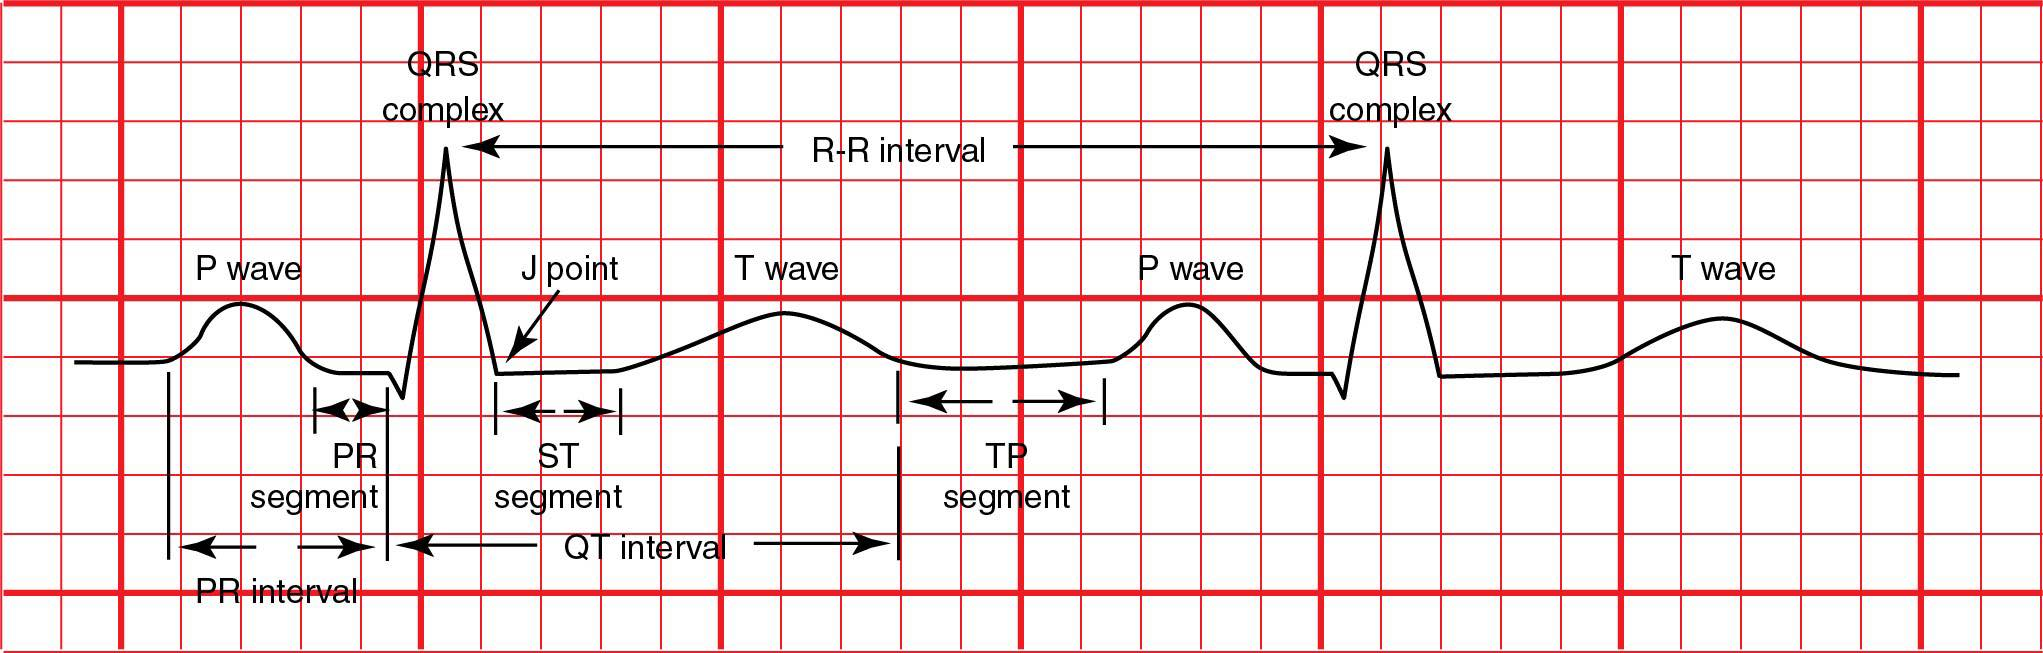
\includegraphics[width=1\linewidth]{images/ecg-huszar.jpg}
\caption{Components of the ECG trace. (\cite{huszar})}
\label{fig:ecg-huszar}
\end{figure}

\noindent Simply said, a 12-lead ECG provides a comprehensive view of the heart's electrical activity from different angles. It consists of 12 different leads, each representing a specific view of the heart. The leads are divided into two main groups: \newline

\noindent \textbf{Limb Leads:}
\begin{itemize}
    \item \textbf{Bipolar Limb Leads:} (Figure \ref{fig:limp})
    \begin{itemize}
        \item \textbf{Lead I:} Measures the voltage difference between the right arm and left arm.
        \item \textbf{Lead II:} Measures the voltage difference between the right arm and left leg.
        \item \textbf{Lead III:} Measures the voltage difference between the left arm and left leg.
    \end{itemize}
    \item \textbf{Augmented Unipolar Limb Leads:} (Figure \ref{fig:augmented})
    \begin{itemize}
        \item \textbf{aVR:} Measures the electrical difference from the right arm to a central point between the left arm and left leg.
        \item \textbf{aVL:} Measures from the left arm to a central point.
        \item \textbf{aVF:} Measures from the left leg to a central point.
    \end{itemize}
\end{itemize}

\begin{figure}[H]
\centering
\begin{minipage}{0.4\linewidth}
    \centering
    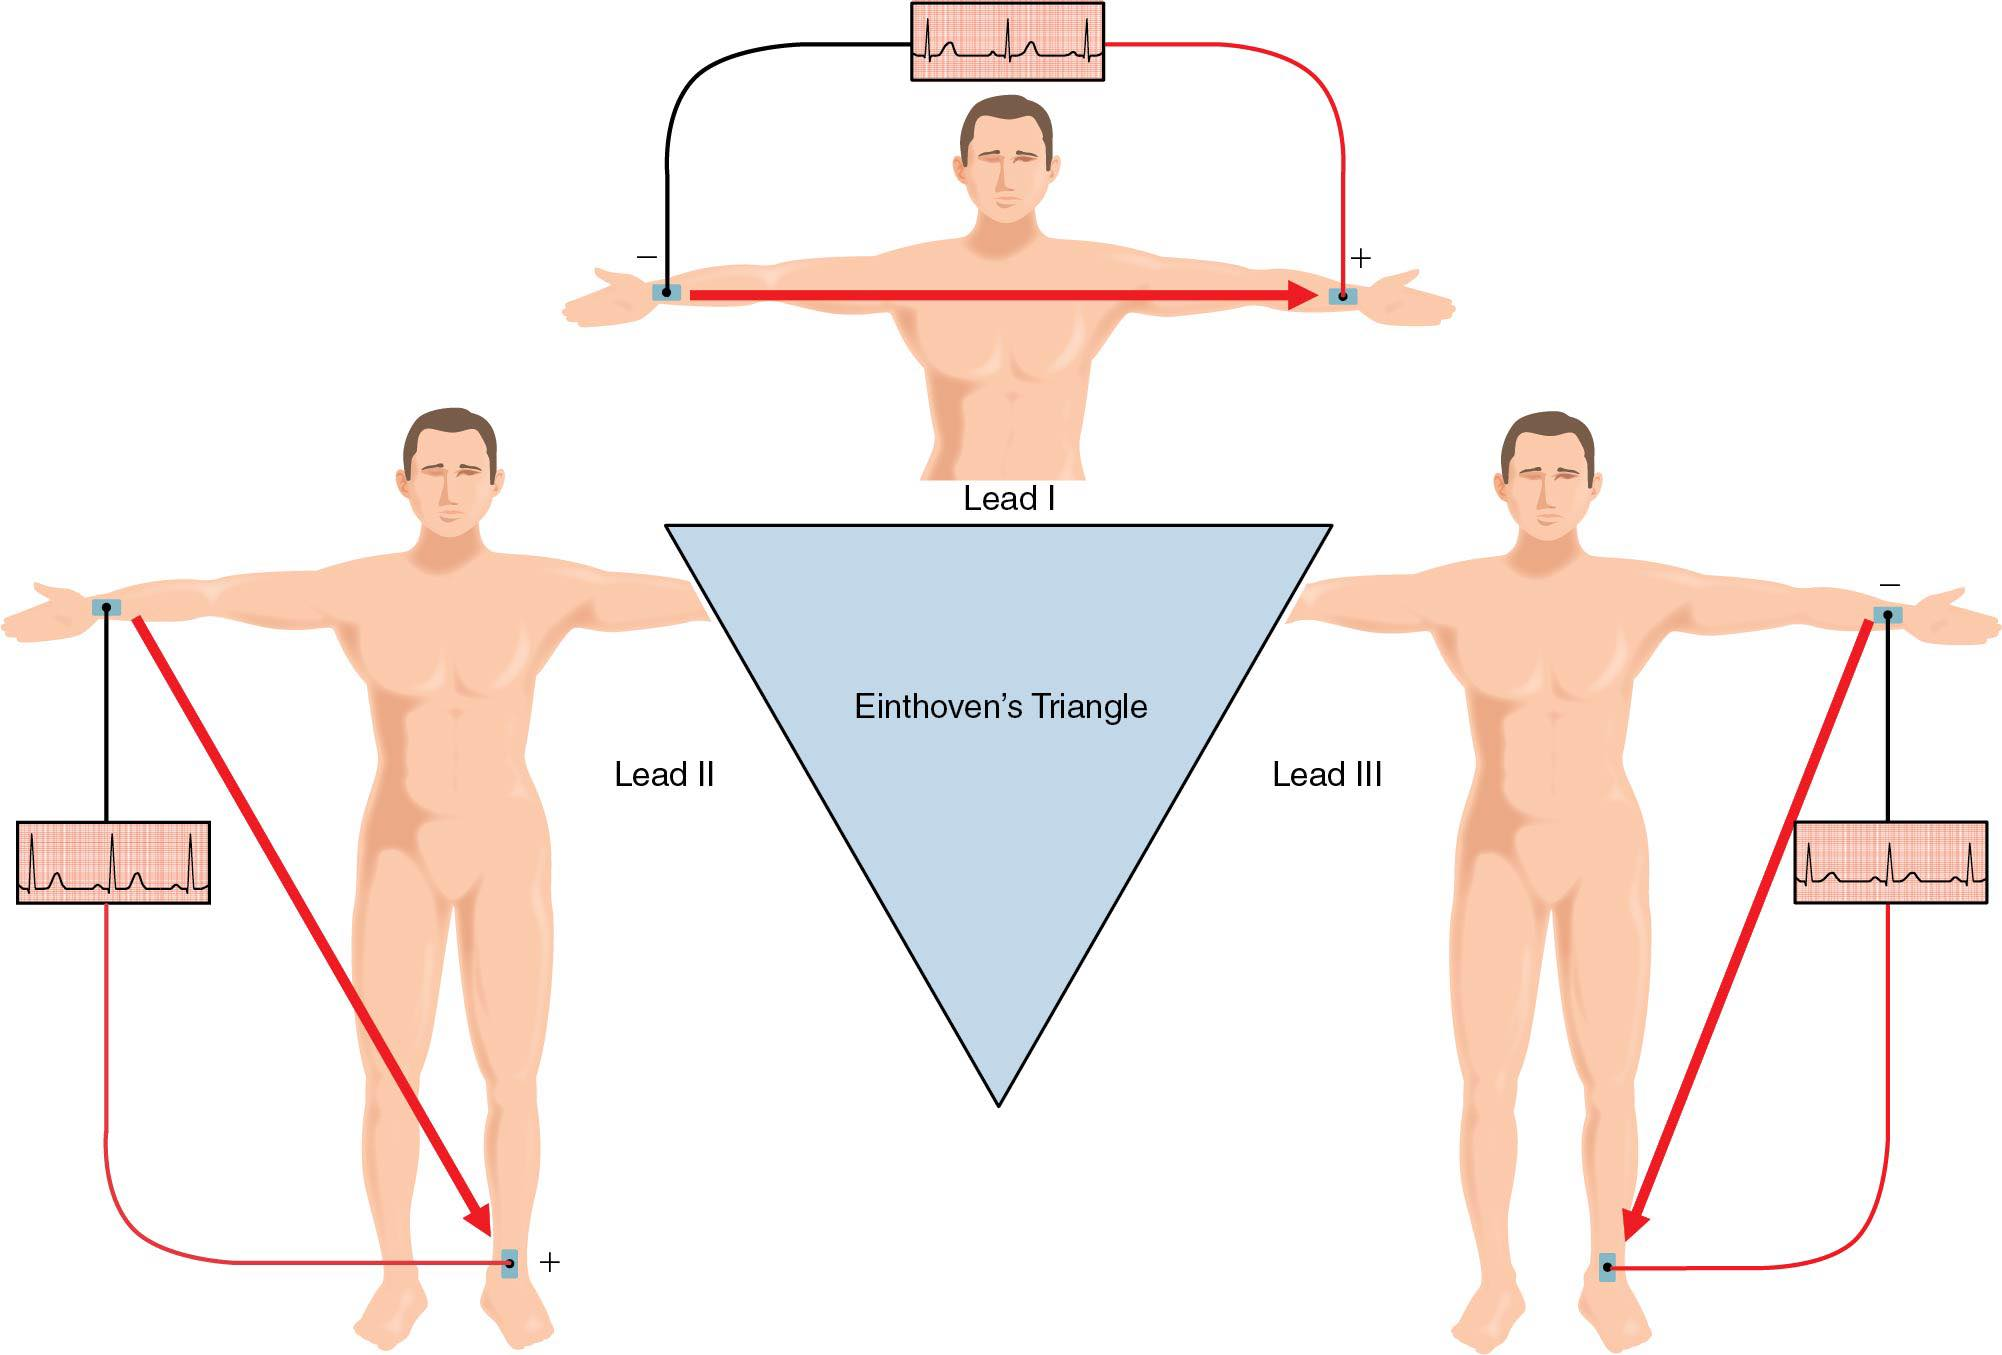
\includegraphics[width=\linewidth]{images/limp-leads-tr.jpg}
    \caption{Bipolar limb leads. (\cite{huszar})}
    \label{fig:limp}
\end{minipage}%
\hspace{0.05\linewidth}
\begin{minipage}{0.4\linewidth}
    \centering
    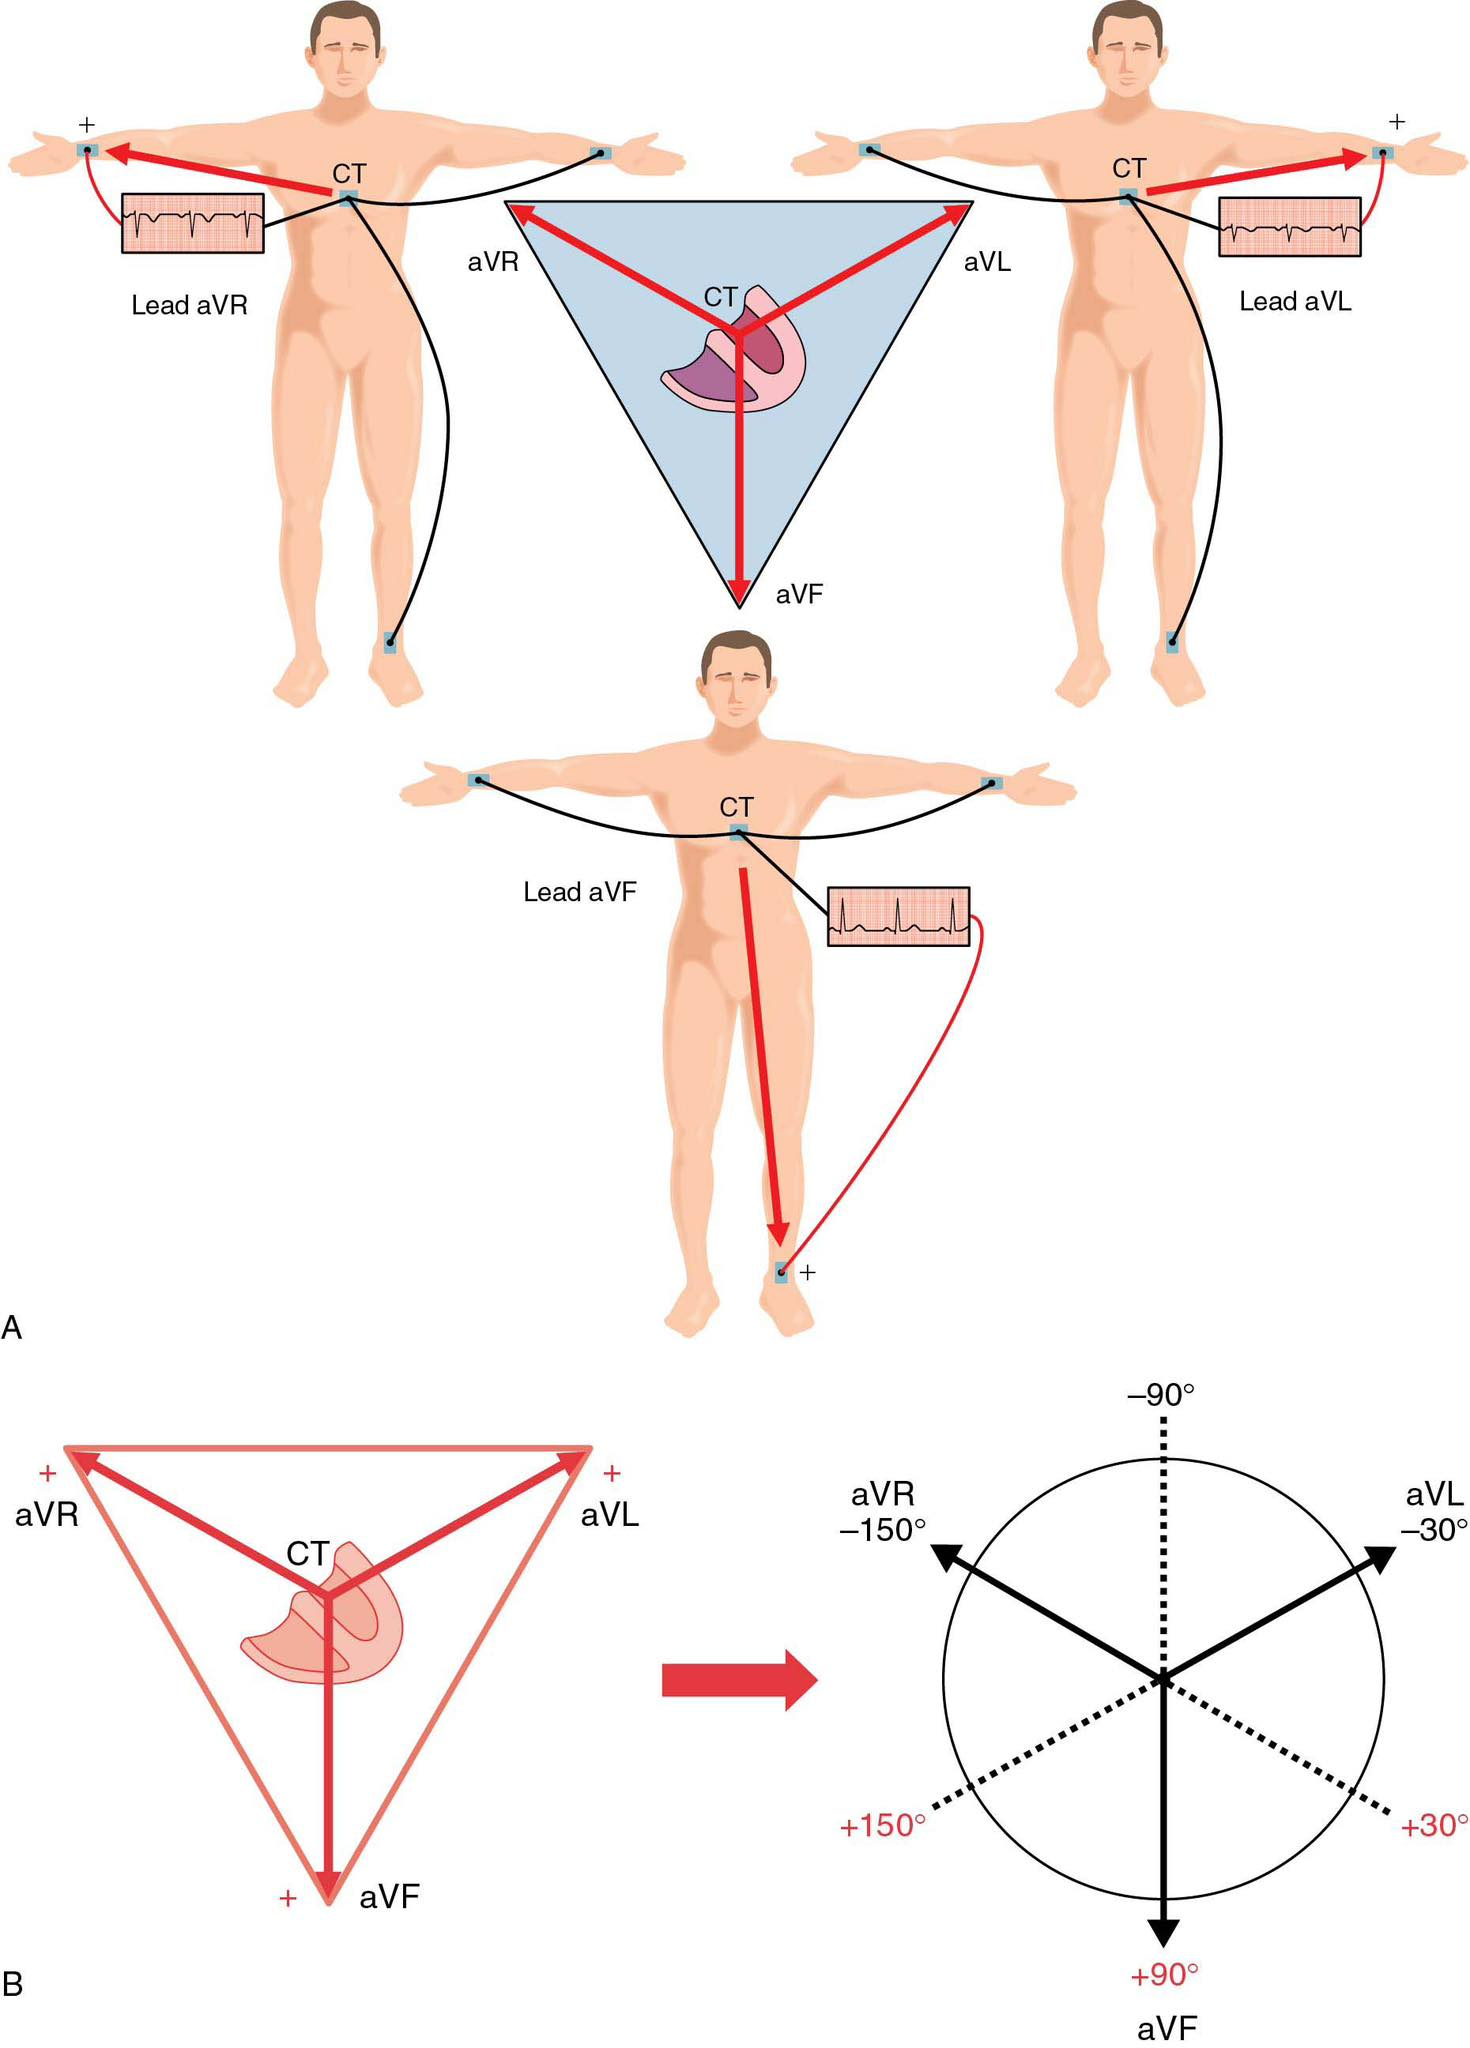
\includegraphics[width=\linewidth]{images/augmented.jpg}
    \caption{Augmented unipolar limb leads. (\cite{huszar})}
    \label{fig:augmented}
\end{minipage}
\end{figure}

\noindent \textbf{Precordial Unipolar Leads:} (Figure \ref{fig:vs})
\begin{itemize}
    \item \textbf{V1 to V6:} These leads provide views of the horizontal plane of the heart, from right to left.
\end{itemize}

\begin{figure}[H]
\centering
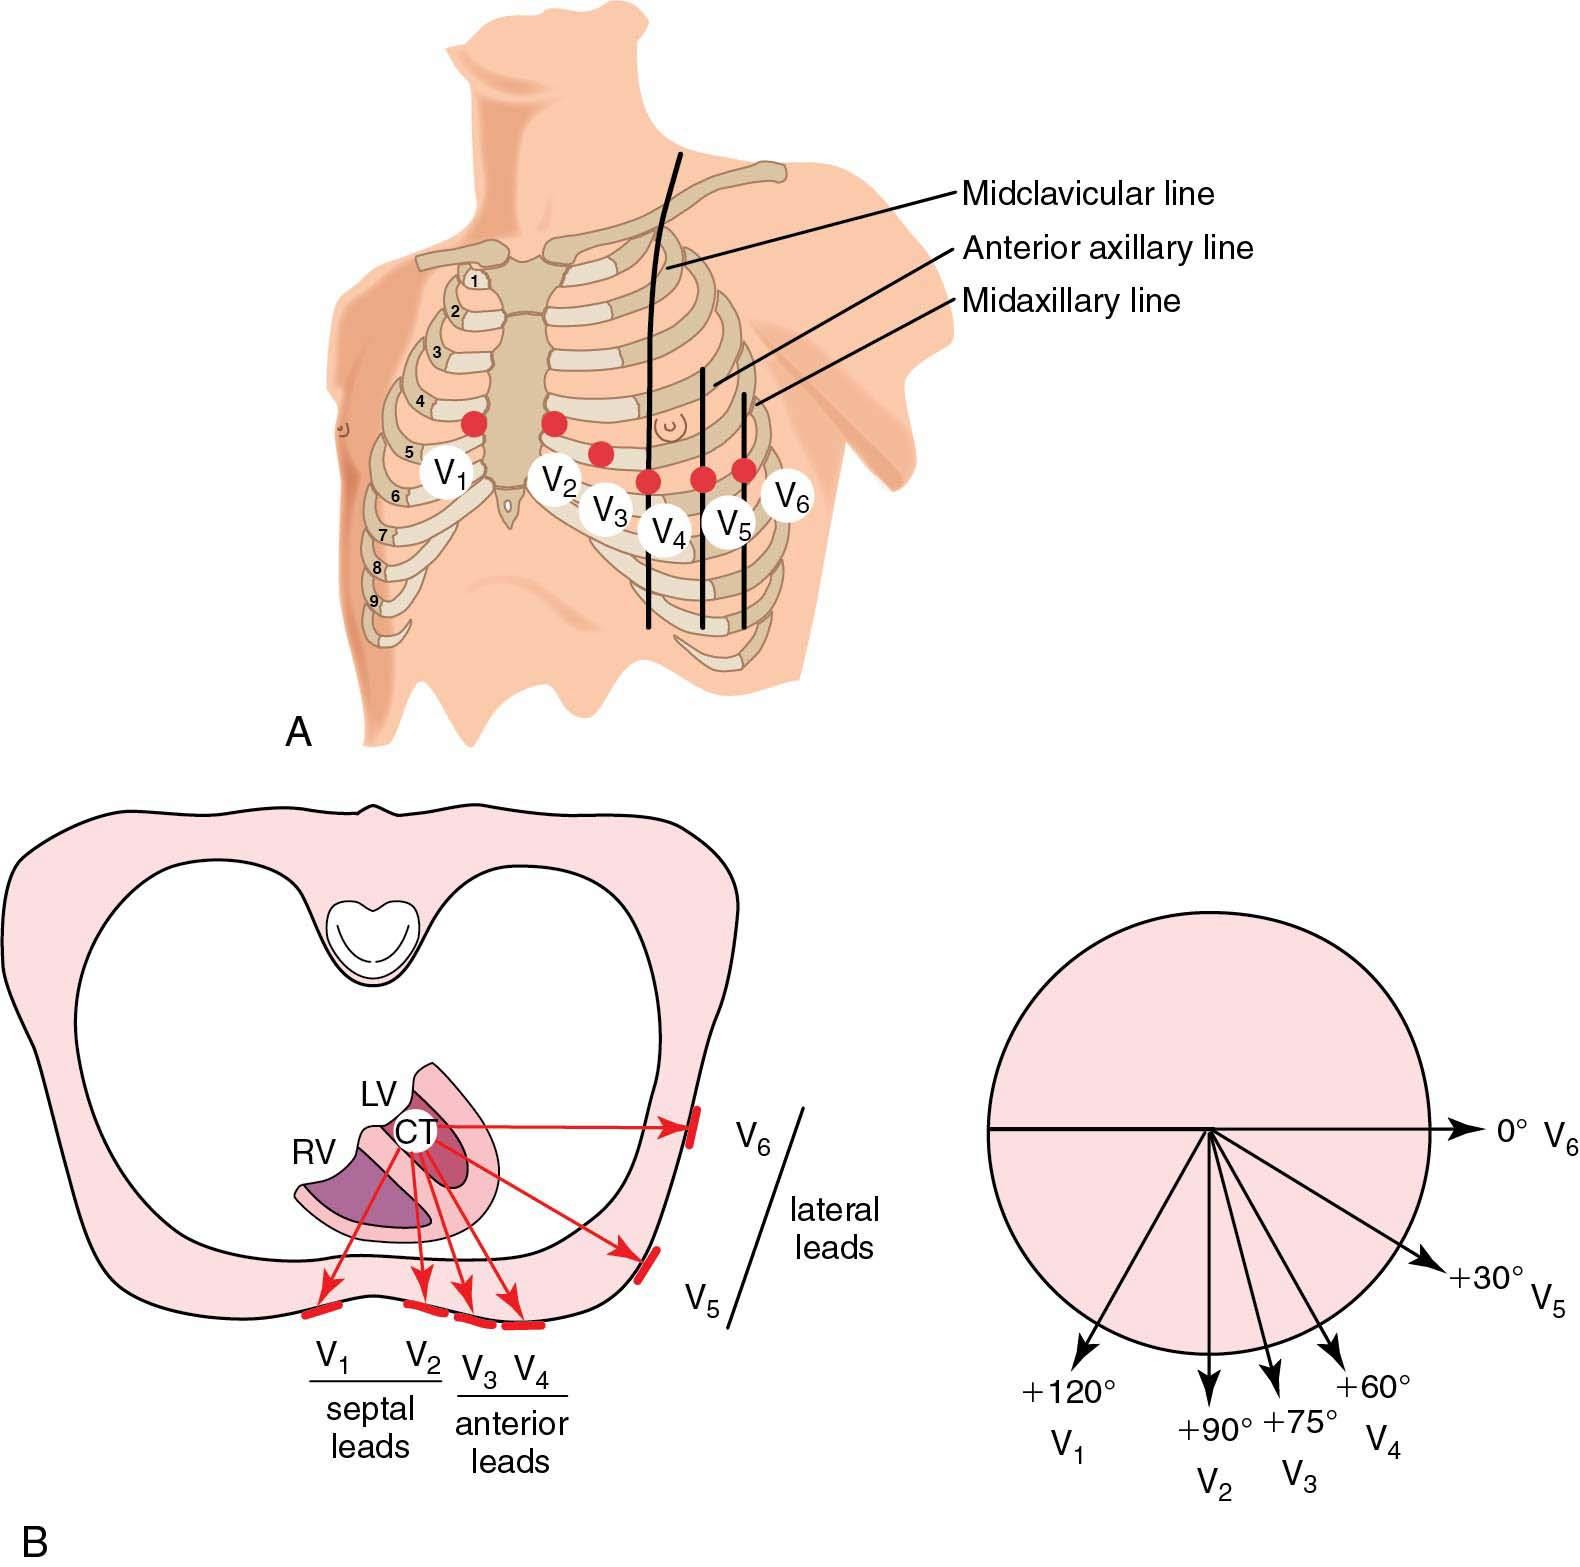
\includegraphics[width=0.5\linewidth]{images/vs.jpg}
\caption{Precordial unipolar leads. (\cite{huszar})}
\label{fig:vs}
\end{figure}

\noindent The so called  \textbf{Einthoven's Triangle} (can be seen in Figure \ref{fig:limp}) is a theoretical formation of the limb leads (I, II, III), forming an equilateral triangle with the heart at the center. This relationship helps in understanding the orientation and magnitude of the heart's electrical activity. The voltages in these leads relate to each other in the following way:

\begin{equation}
    \text{Lead I} + \text{Lead III} = \text{Lead II}.
\end{equation}

\noindent The voltages in augmented limb leads are calculated by amplifying the electrical difference between one limb electrode and a central point formed by the other limb electrodes. These relationships are based on the principle that the sum of the voltages from all three limb leads should be zero when the heart's electrical axis is normal.

% forcing a page break
\clearpage

\chapter{Experiments and Results} \label{ch:3}

For the experiments we are going to use the already available dataser "A Large Scale 12-lead Electrocardiogram Database for Arrhythmia Study" (\cite{cite1}, \cite{cite2}, \cite{cite3}). This is a comprehensive database of high-quality 12-lead ECG signals collected from $45 152$ patients. Each signal is with length of $10$ seconds corresponding to $5 000$ data points. The dataset is designed to support arrhythmia research, containing labeled data for various cardiac conditions such as atrial fibrillation, premature ventricular contractions, and bundle branch blocks. This large dataset has high-quality labels from professional experts, diverse arrhythmia types, and additional cardiovascular conditions, making it suitable for performing our tests on it. \newline


% • Presents a comprehensive database of 12-lead ECG signals collected from 45,152 patients. Each signal is with length of 10 seconds corresponding to 5000 data points.
% • The dataset is designed to support arrhythmia research, containing labeled data for various cardiac conditions such as atrial fibrillation, premature ventricular contractions, and bundle branch blocks.
% • ECG data is non-invasive and critical for diagnosing cardiovascular conditions, but analyzing such large
% datasets requires efficient automated methods.
% • Large dataset, high-quality labels from professional experts, diverse arrhythmia types, and additional cardiovascular conditions. \newline


% Pre,post, processing

% What exactly is tested - 5k points, sample from the points, results, smoothing, no smoothing, differеnt ranks, fourier terms

\section{Missing Data Imputation}

In this section, we evaluate PSMF and rPSMF on the task of imputing missing values in 12-lead ECG time-series data. The 12-lead ECG signal is chosen to be one representing a normal heart rhythm (sinus rhythm). As already mentioned each of the $m = 12$ leads contains $n = 5000$ data points. One heart beat (PQRST complex) is of apprixamte lebgth of $300$ data points. That's why, to assess the imputation accuracy, we choose to randomly remove segments of length $300$ from the signal, and construct datasets with $20\%$, $30\%$, and $40\%$ missing data. We compare the results for each dataset against two other baseline sequential methods used in the PSMF paper (\cite{akyildiz2021probabilistic}). The first, which we call MLE-SMF, is a maximum likelihood estimation (MLE) method for online probabilistic matrix factorization where the state transition matrix $C$ remains constant over time. This builds on prior work by \cite{YILDIRIM2012494}, \cite{6288274}, and \cite{6638240}. The second approach adapts the temporal matrix factorization (TMF) optimization technique proposed by \cite{NIPS2016_85422afb}. \newline

\noindent For PSMF and rPSMF we choose a random walk subspace model $f_{\theta}(x) = x$, and for the imputation we use the final estimates of $C$ and $X$. We test the four sequential models by setting the rank first to $r = 3$, and then to $r = 10$. As in \cite{akyildiz2021probabilistic}, for TMF we set the weight matrix to identity, for PSMF and MLE- SMF we set $R_k := R = \rho \otimes I_r$, where $\rho = 10$, $P_0 = I_r$, $Q_k := Q = q \otimes I_r$, and $q = 0.1$. For rPSMF we use $R_0 = R$ and $Q_0 = Q$ and choose $\lambda_0 = 1.8$, and for both PSMF and rPSMF we set $V_0 = v_0 \otimes I_r$ with $v_0 = 2$. We evaluate the performance of the four methods - PSMF, rPSMF, MLE-SMF, and TMF - by running each of them for two epochs. To ensure the robustness and reliability of our findings, we conduct the experiments $100$ times, each time using different initializations and randomly generated patterns of missing data. \newline

\noindent In Table \ref{tab:rmse3} we can see the results for $r = 3$. We see that PSMF and rPSMF have lower RMSEs compared to MLE-SMF and TMF.  \newline

\begin{table}[H]
\centering
\label{tab:rmse3}
\text{$r = 3$} \\[0.5ex]
\begin{tabular}{@{}lccc|ccccc@{}}
\toprule
 & \multicolumn{3}{c}{Imputation RMSE} & \multicolumn{3}{c}{Runtime (s)} \\
 & 20\% & 30\% & 40\% & 20\% & 30\% & 40\% \\
\midrule
PSMF & $\underset{{\scriptscriptstyle \;\;(32.19)}}{104.46}$ & $\underset{{\scriptscriptstyle \;\;(31.61)}}{115.99}$ & $\underset{{\scriptscriptstyle \;\;\;(31.77)}}{138.18}$ & 0.58 & 0.59 & 0.58 \\
rPSMF & $\underset{{\scriptscriptstyle \;\;(26.56)}}{\textbf{98.51}}$ & $\underset{{\scriptscriptstyle \;\;(29.08)}}{\textbf{109.04}}$ & $\underset{{\scriptscriptstyle \;\;(29.58)}}{\textbf{124.91}}$ & 0.65 & 0.64 & 0.64 \\
MLE-SMF & $\underset{{\scriptscriptstyle \;\;\;(34.07)}}{271.04}$ & $\underset{{\scriptscriptstyle \;\;\;(33.46)}}{263.65}$ & $\underset{{\scriptscriptstyle \;\;\;(28.69)}}{244.21}$ & 0.50 & 0.51 & 0.50 \\
TMF & $\underset{{\scriptscriptstyle \;\;\;(16.18)}}{202.76}$ & $\underset{{\scriptscriptstyle \;\;\;(15.97)}}{202.90}$ & $\underset{{\scriptscriptstyle \;\;\;(19.24)}}{208.98}$ & 0.28 & 0.28 & 0.27 \\
\bottomrule
\end{tabular}
\caption{Imputation error and runtime using 20\%, 30\% and 40\% missing values, rank 3, averaged over 100 random repetitions.}
\end{table}

\begin{table}[H]
\centering
\label{tab:rmse10}
\text{$r = 10$} \\[0.5ex]
\begin{tabular}{@{}lccc|ccccc@{}}
\toprule
 & \multicolumn{3}{c}{Imputation RMSE} & \multicolumn{3}{c}{Runtime (s)} \\
 & 20\% & 30\% & 40\% & 20\% & 30\% & 40\% \\
\midrule
PSMF & $\underset{{\scriptscriptstyle \;\;(38.89)}}{\textbf{122.79}}$ & $\underset{{\scriptscriptstyle \;\;(45.69)}}{\textbf{154.79}}$ & $\underset{{\scriptscriptstyle \;\;\;(52.85)}}{\textbf{186.31}}$ & 0.92 & 1.07 & 1.07 \\
rPSMF & $\underset{{\scriptscriptstyle \;\;(71.96)}}{192.19}$ & $\underset{{\scriptscriptstyle \;\;(92.27)}}{253.77}$ & $\underset{{\scriptscriptstyle \;\;(132.56)}}{377.75}$ & 1.10 & 1.08 & 1.07\\
MLE-SMF & $\underset{{\scriptscriptstyle \;\;\;(21.63)}}{268.57}$ & $\underset{{\scriptscriptstyle \;\;\;(30.37)}}{267.81}$ & $\underset{{\scriptscriptstyle \;\;\;(33.82)}}{270.77}$ & 0.82 & 0.90 & 0.90 \\
TMF & $\underset{{\scriptscriptstyle \;\;\;(20.04)}}{205.67}$ & $\underset{{\scriptscriptstyle \;\;\;(17.31)}}{199.81}$ & $\underset{{\scriptscriptstyle \;\;\;(20.25)}}{193.28}$ & 0.42 & 0.47 & 0.44 \\
\bottomrule
\end{tabular}
\caption{Imputation error and runtime using 20\%, 30\% and 40\% missing values, rank 10, averaged over 100 random repetitions.}
\end{table}

\noindent We can also measure the proportion of missing values that lie within a $2\sigma$ coverage interval of the approximate posterior distribution. Table 3 shows how our method improves over the uncertainty quantification of MLE-SMF (the other methods do not provide a posterior distribution). This illustrates the added value of the matrix-variate prior on C, as well as our inference scheme. Note that rPSMF obtains a higher coverage percentage than PSMF on three of the datasets, which is due to the sequential updating of the noise covariances. \newline

\begin{table}[H]
    \centering
    \begin{minipage}{0.45\textwidth}
        \centering
        \text{$r = 3$} \\[0.5ex]
        \begin{threeparttable}
            \begin{tabular}{lccc}
                \hline
                Missing \%: & 20\% & 30\% & 40\% \\
                \hline
                PSMF & 0.14 & 0.12 & 0.10 \\
                rPSMF & \textbf{0.80} & \textbf{0.75} & \textbf{0.66} \\
                MLE-SMF & 0.07 & 0.06 & 0.06 \\
                \hline
            \end{tabular}
        \end{threeparttable}
    \end{minipage}%
    \hspace{0.1\textwidth}%
    \begin{minipage}{0.45\textwidth}
        \centering
        \text{$r = 10$} \\[0.5ex]
        \begin{threeparttable}
            \begin{tabular}{lccc}
                \hline
                Missing \%: & 20\% & 30\% & 40\% \\
                \hline
                PSMF & 0.24 & 0.18 & 0.14 \\
                rPSMF & \textbf{0.60} & \textbf{0.50} & \textbf{0.37} \\
                MLE-SMF & 0.07 & 0.06 & 0.05 \\
                \hline
            \end{tabular}
        \end{threeparttable}
    \end{minipage}
    \caption{Average coverage proportion of the missing data by the $2\sigma$ uncertainty bars of the posterior predictive estimates, averaged over 100 repetitions. Left: results for rank 3, right: results for rank 10.}
\end{table}

% \begin{figure}[H]
% \centering
% \includegraphics[width=0.75\linewidth]{images/missing/psmf_output_300_20_3.pdf}
% \caption{Input with 300 missing data points per wave.}
% \label{fig:vs}
% \end{figure}

% \begin{figure}[H]
% \centering
% \includegraphics[width=0.75\linewidth]{images/missing/rpsmf_output_300_20_3.pdf}
% \caption{Input with 300 missing data points per wave.}
% \label{fig:vs}
% \end{figure}

\begin{figure}[H]
\centering
\begin{minipage}{0.4\linewidth}
    \centering
    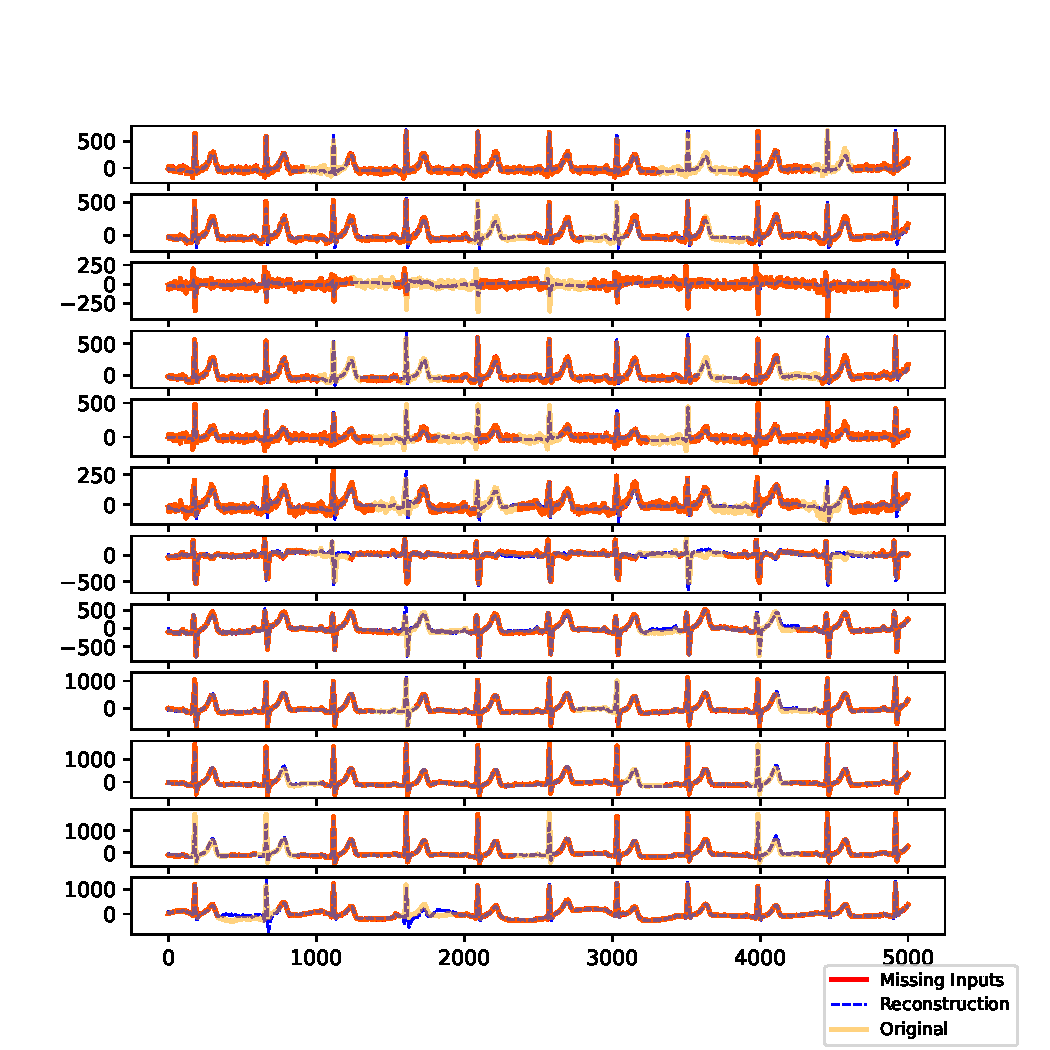
\includegraphics[width=\linewidth]{images/missing/psmf_output_20_3.pdf}
\end{minipage}%
\hspace{0.05\linewidth}
\begin{minipage}{0.4\linewidth}
    \centering
    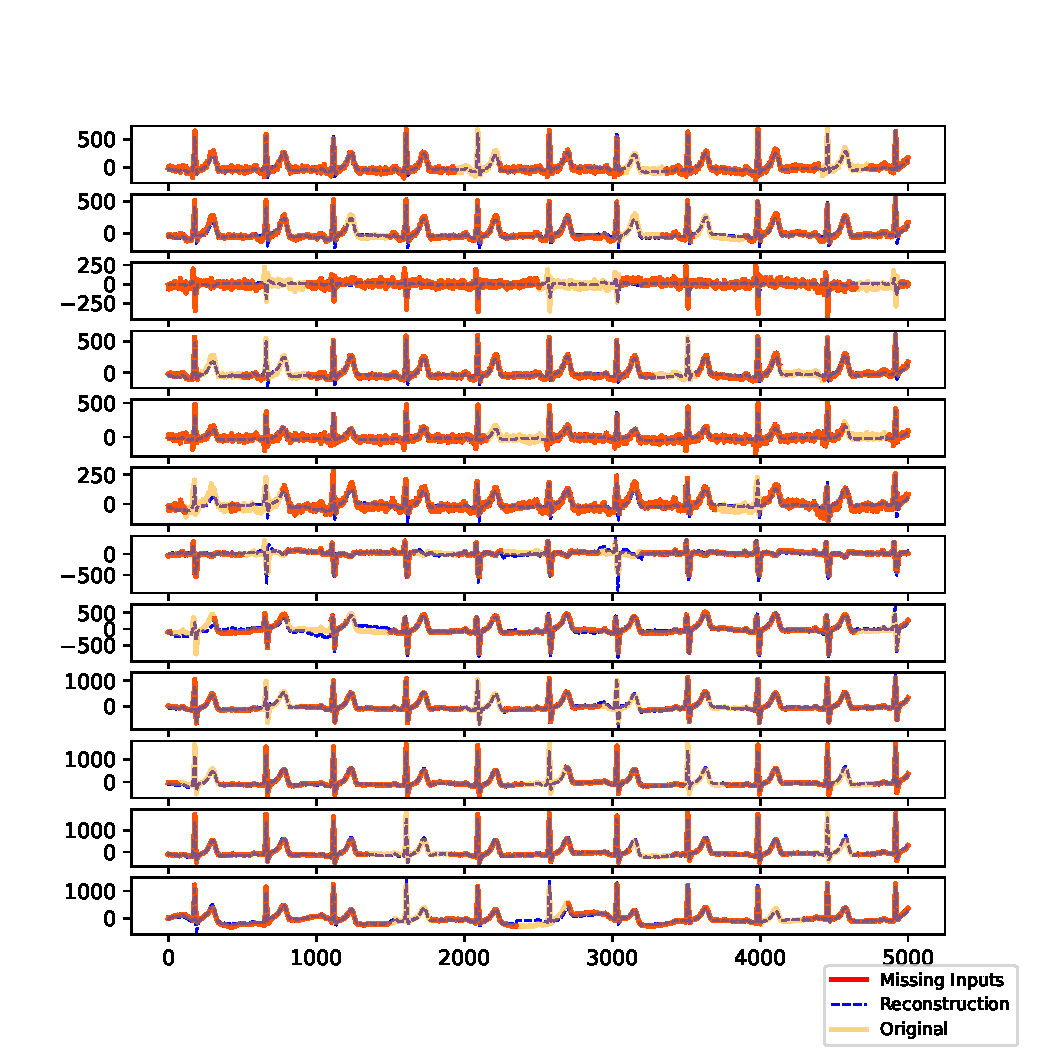
\includegraphics[width=\linewidth]{images/missing/rpsmf_output_20_3.pdf}
\end{minipage}
\caption{Reconstruction with rank 3 of 20\% missing data. Left: PSMF; Right: rPSMF.}
\end{figure}

\begin{figure}[H]
\centering
\begin{minipage}{0.4\linewidth}
    \centering
    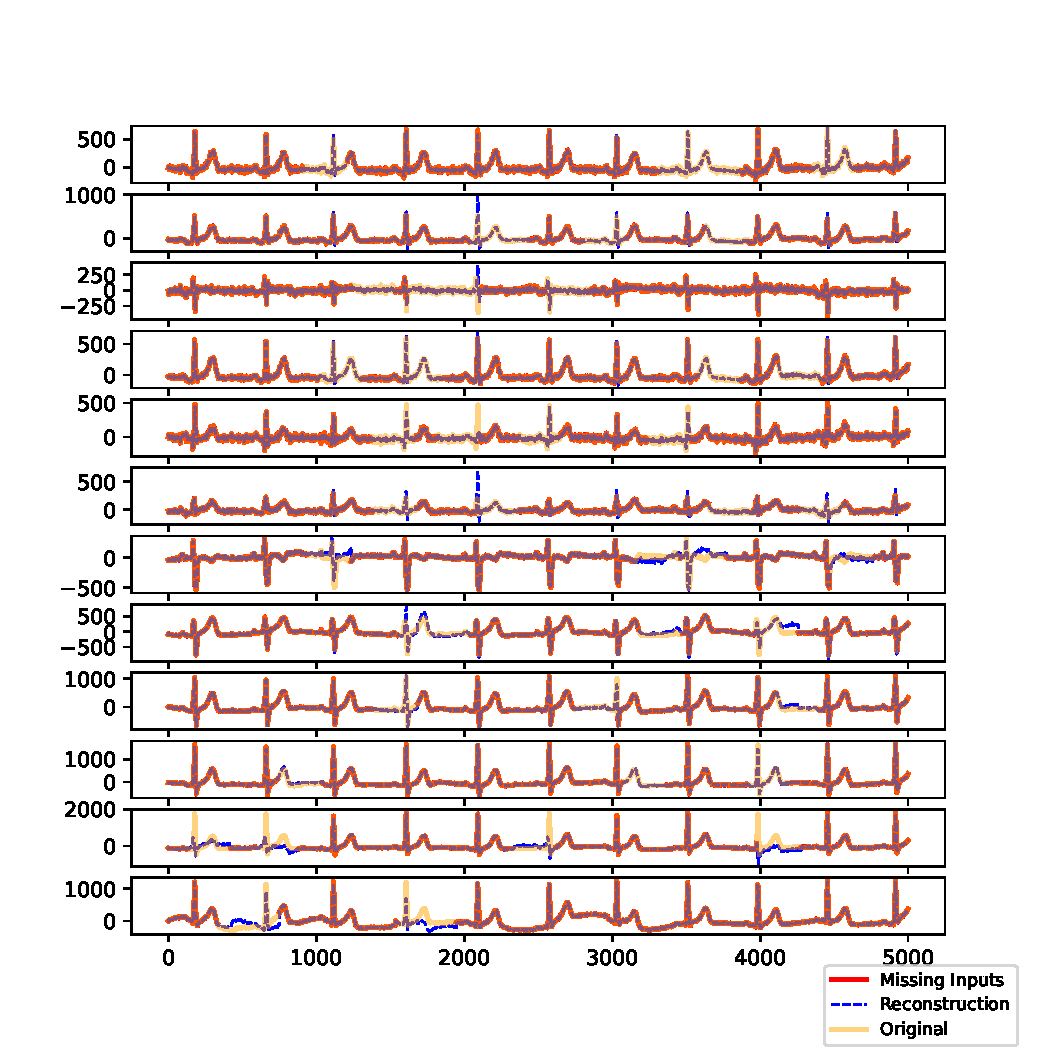
\includegraphics[width=\linewidth]{images/missing/psmf_output_20_10.pdf}
    \label{fig:limp}
\end{minipage}%
\hspace{0.05\linewidth}
\begin{minipage}{0.4\linewidth}
    \centering
    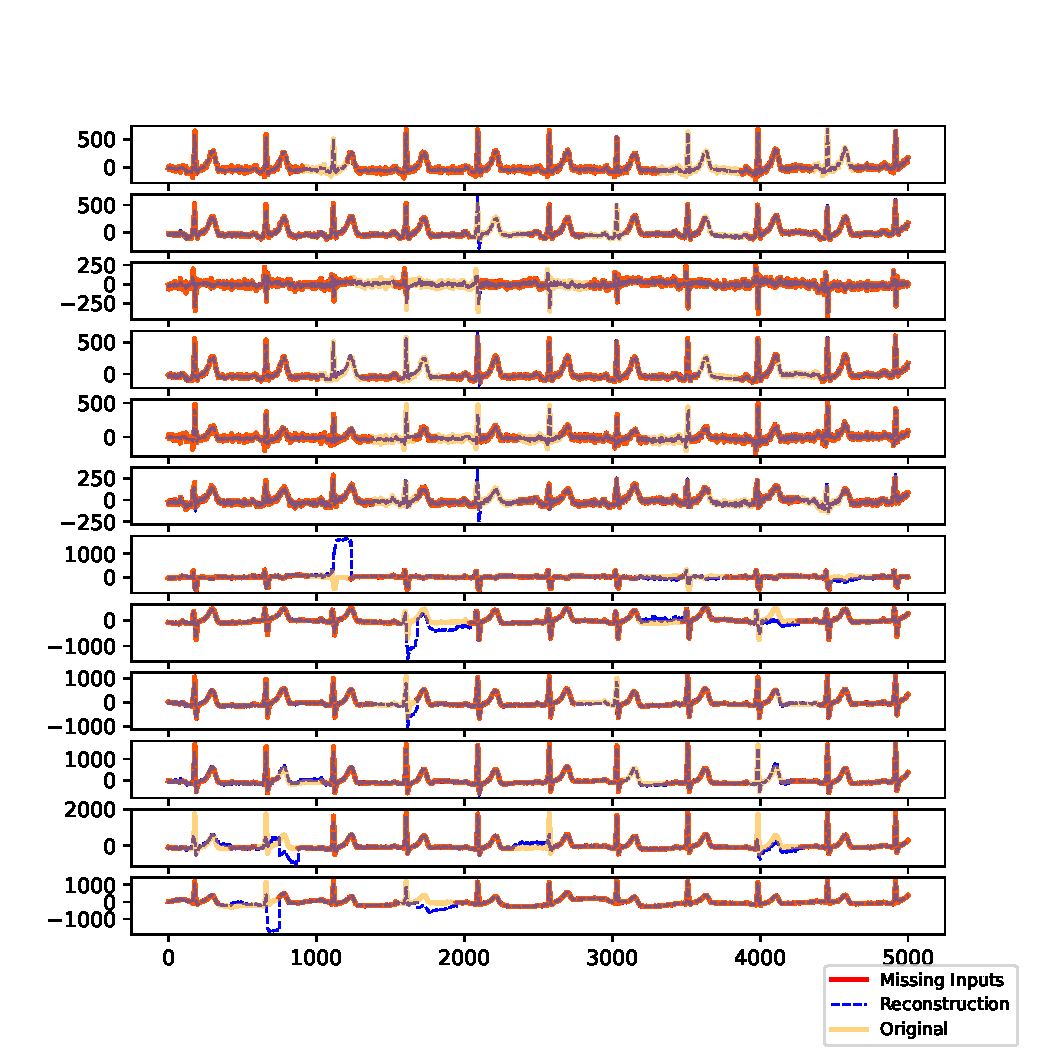
\includegraphics[width=\linewidth]{images/missing/rpsmf_output_20_10.pdf}
    \label{fig:augmented}
\end{minipage}
\caption{Reconstruction with rank 10, 20\% coverage. Left: PSMF; Right: rPSMF.}
\end{figure}

\noindent TODO: add more results. here or in the appendix/supplement?

\section{R-peaks Detection}

TODO:
\begin{itemize}
    \item intro: why it is an important task, mention current methods?
    \item introduce the idea: smoother peaks, remove reconstruction from the original data
    \item threshold
    \item (potential) issues, improvements, results
    \item figure caption, more result figures
    \item add the real r peaks in circles on the plots
\end{itemize}

\begin{figure}[H]
\centering
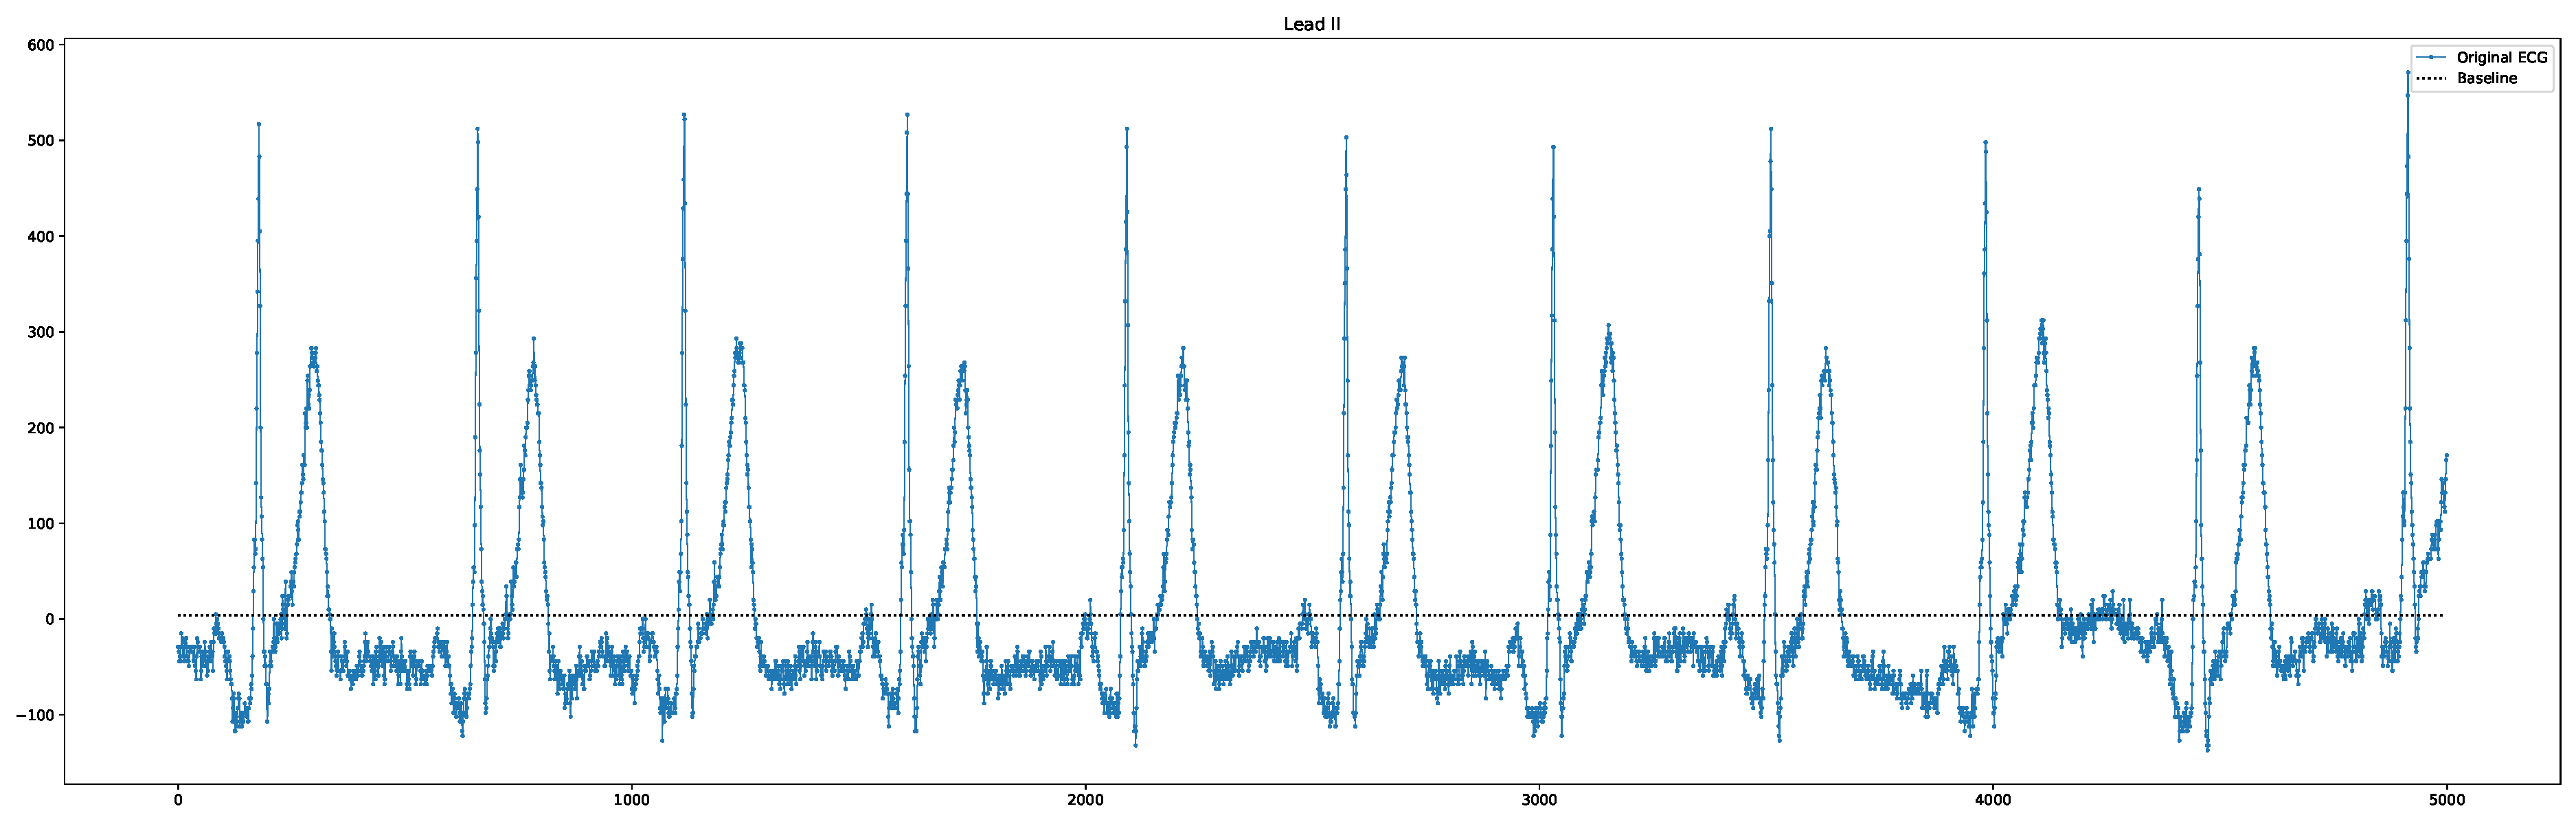
\includegraphics[width=1\linewidth]{images/r_peaks/original_ecg_m.pdf}
\caption{Original Lead II signal, 5000 points.}
\label{fig:orig-ecg}
\end{figure}

\begin{figure}[H]
\centering
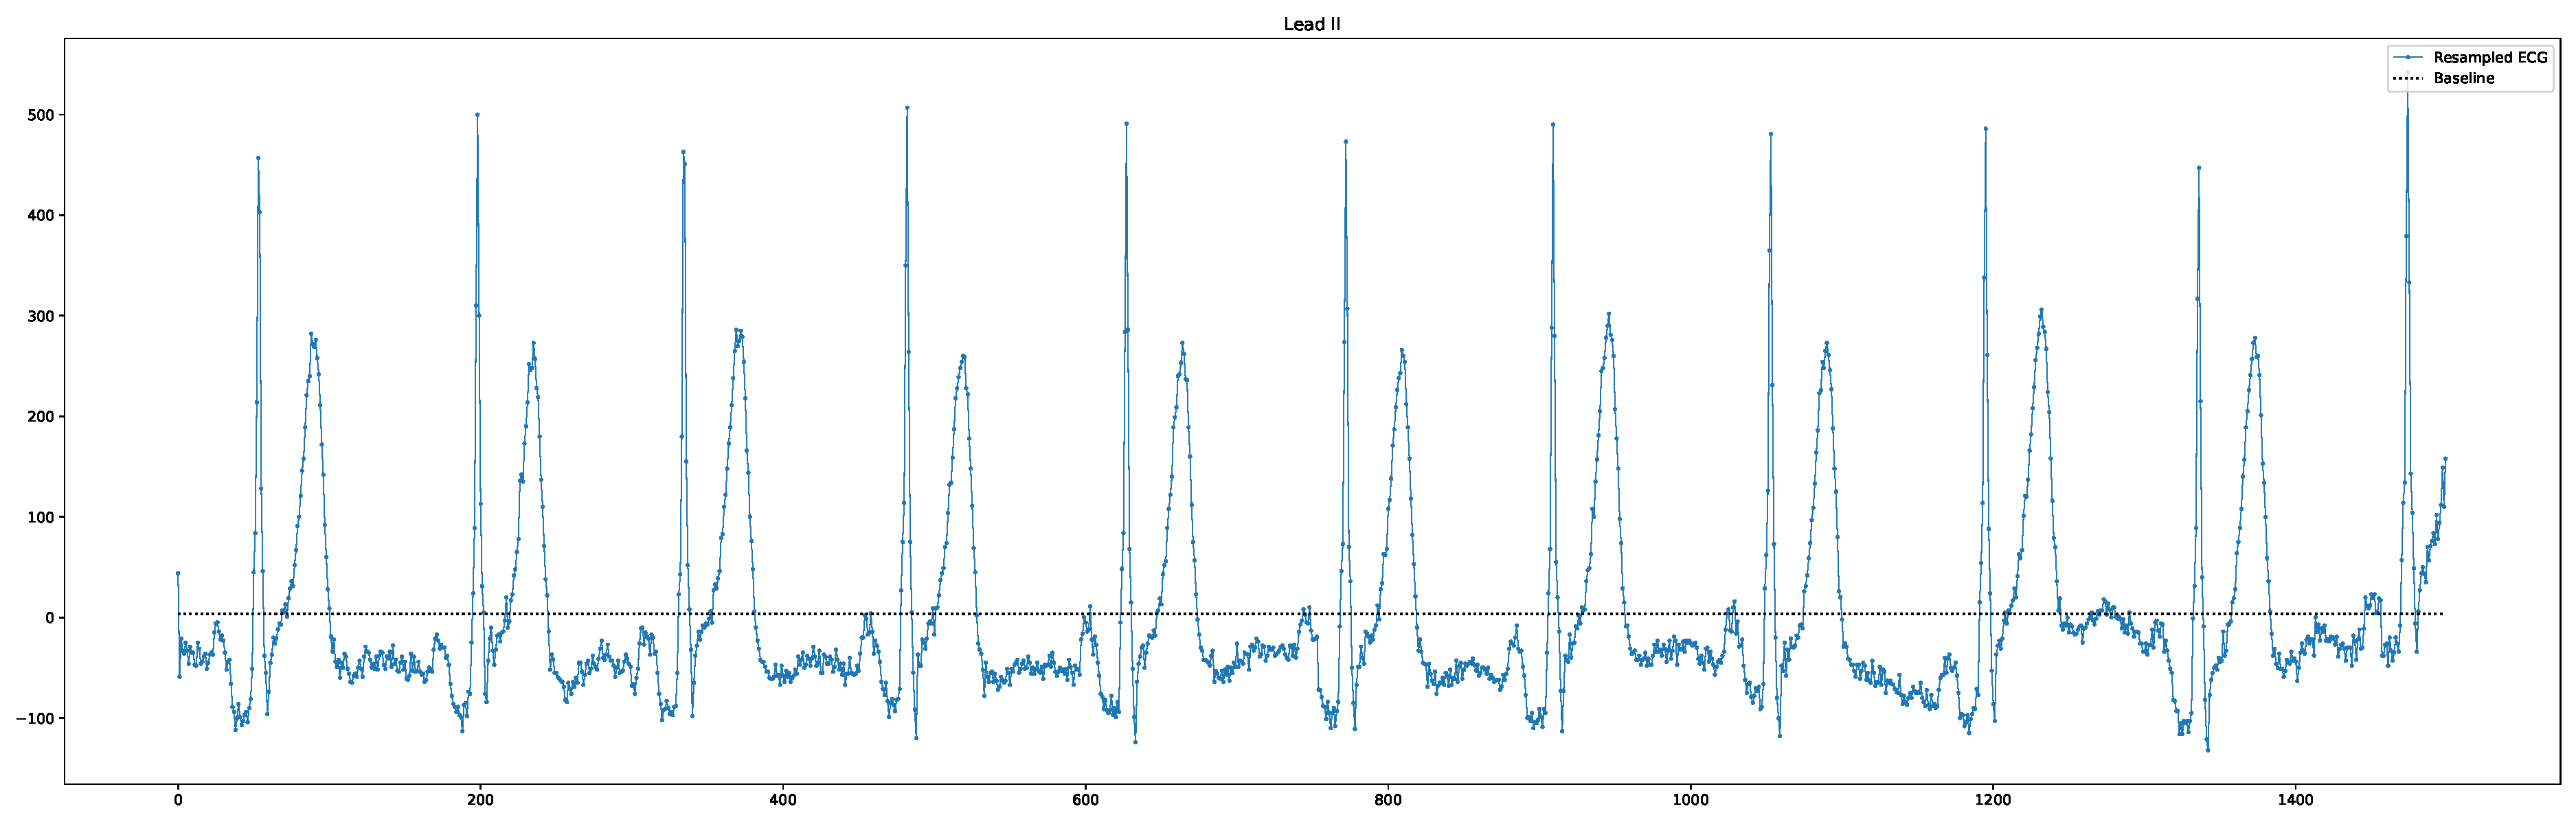
\includegraphics[width=1\linewidth]{images/r_peaks/resampled_ecg_m.pdf}
\caption{Resampled Lead II signal, 1500 points.}
\label{fig:resampled-ecg}
\end{figure}

\begin{figure}[H]
\centering
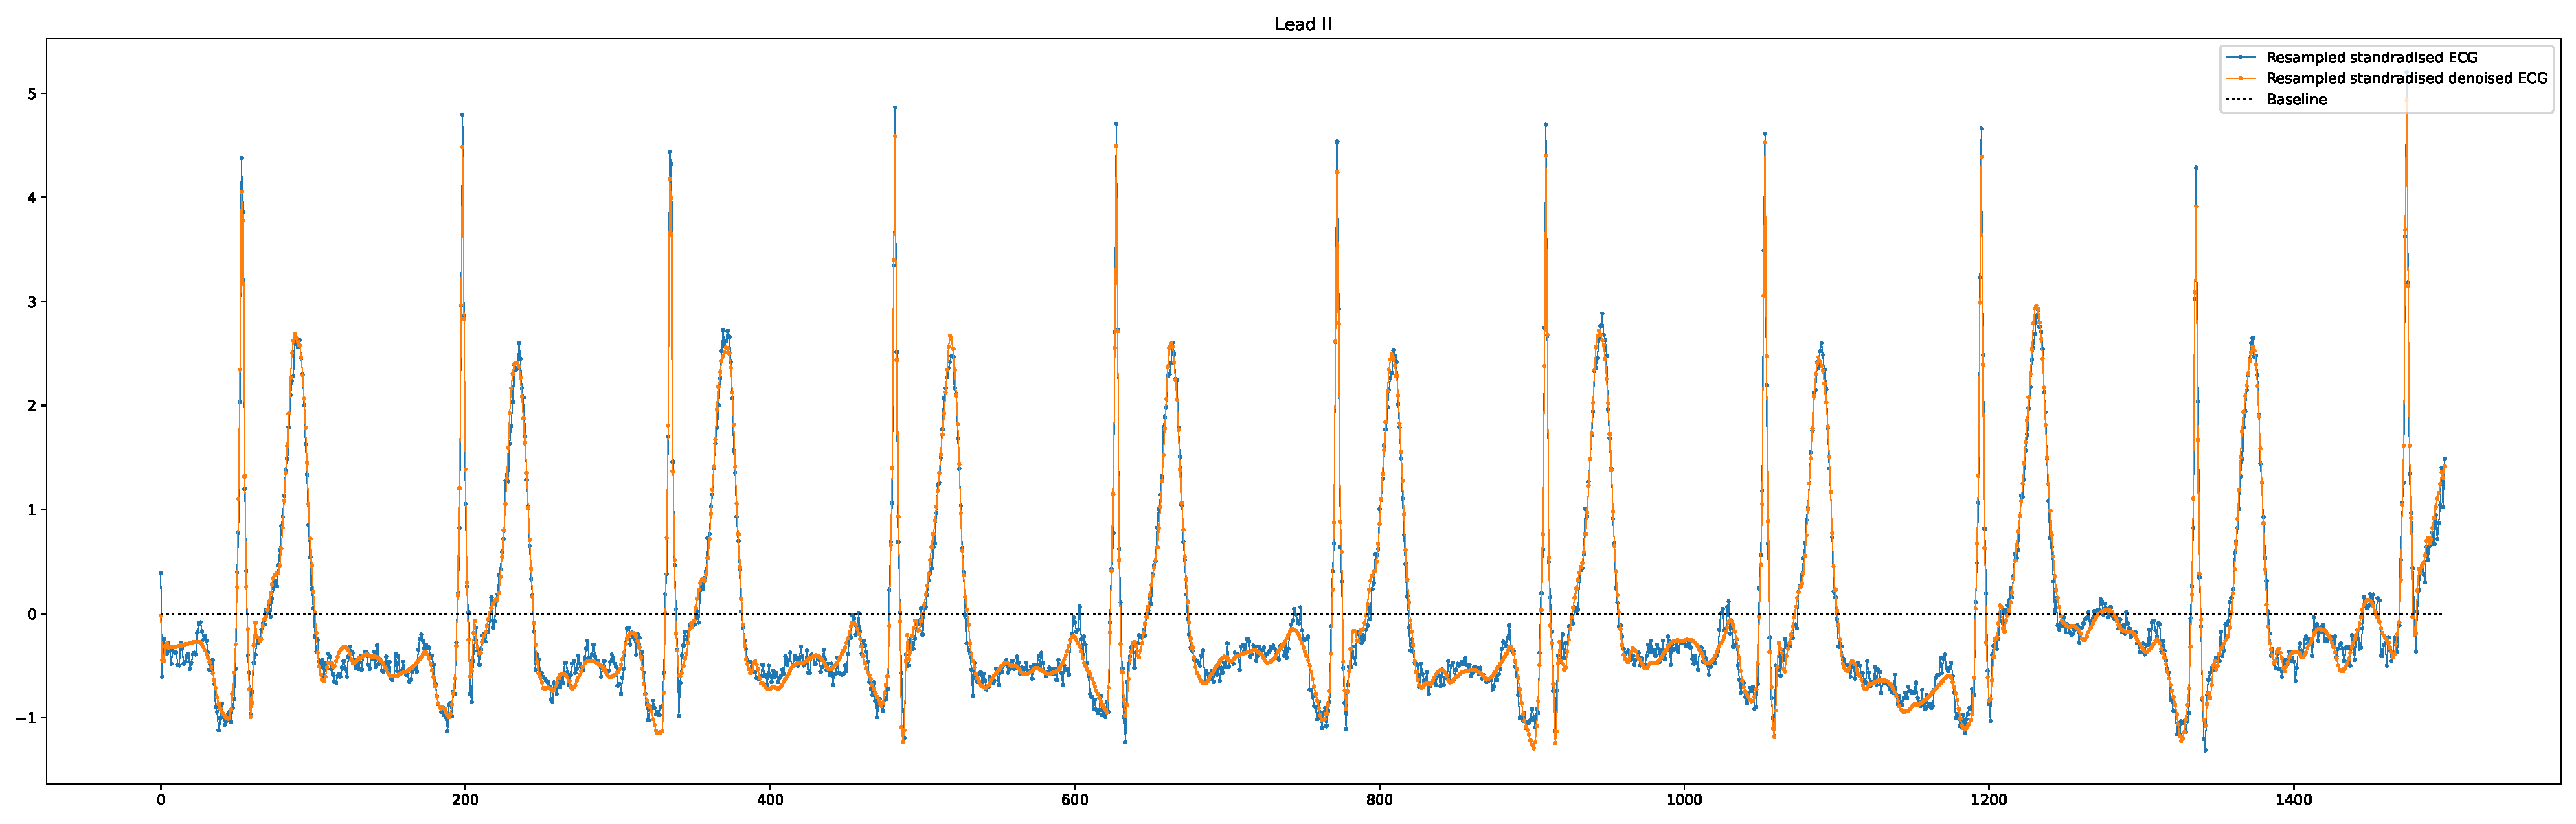
\includegraphics[width=1\linewidth]{images/r_peaks/resampled_standardised_denoised_ecg_m.pdf}
\caption{Resampled Lead II signal (blue), and the denoised version (orange) of the same signal after applying wavelet transform.}
\label{fig:res-st-den-ecg}
\end{figure}

\begin{figure}[H]
\centering
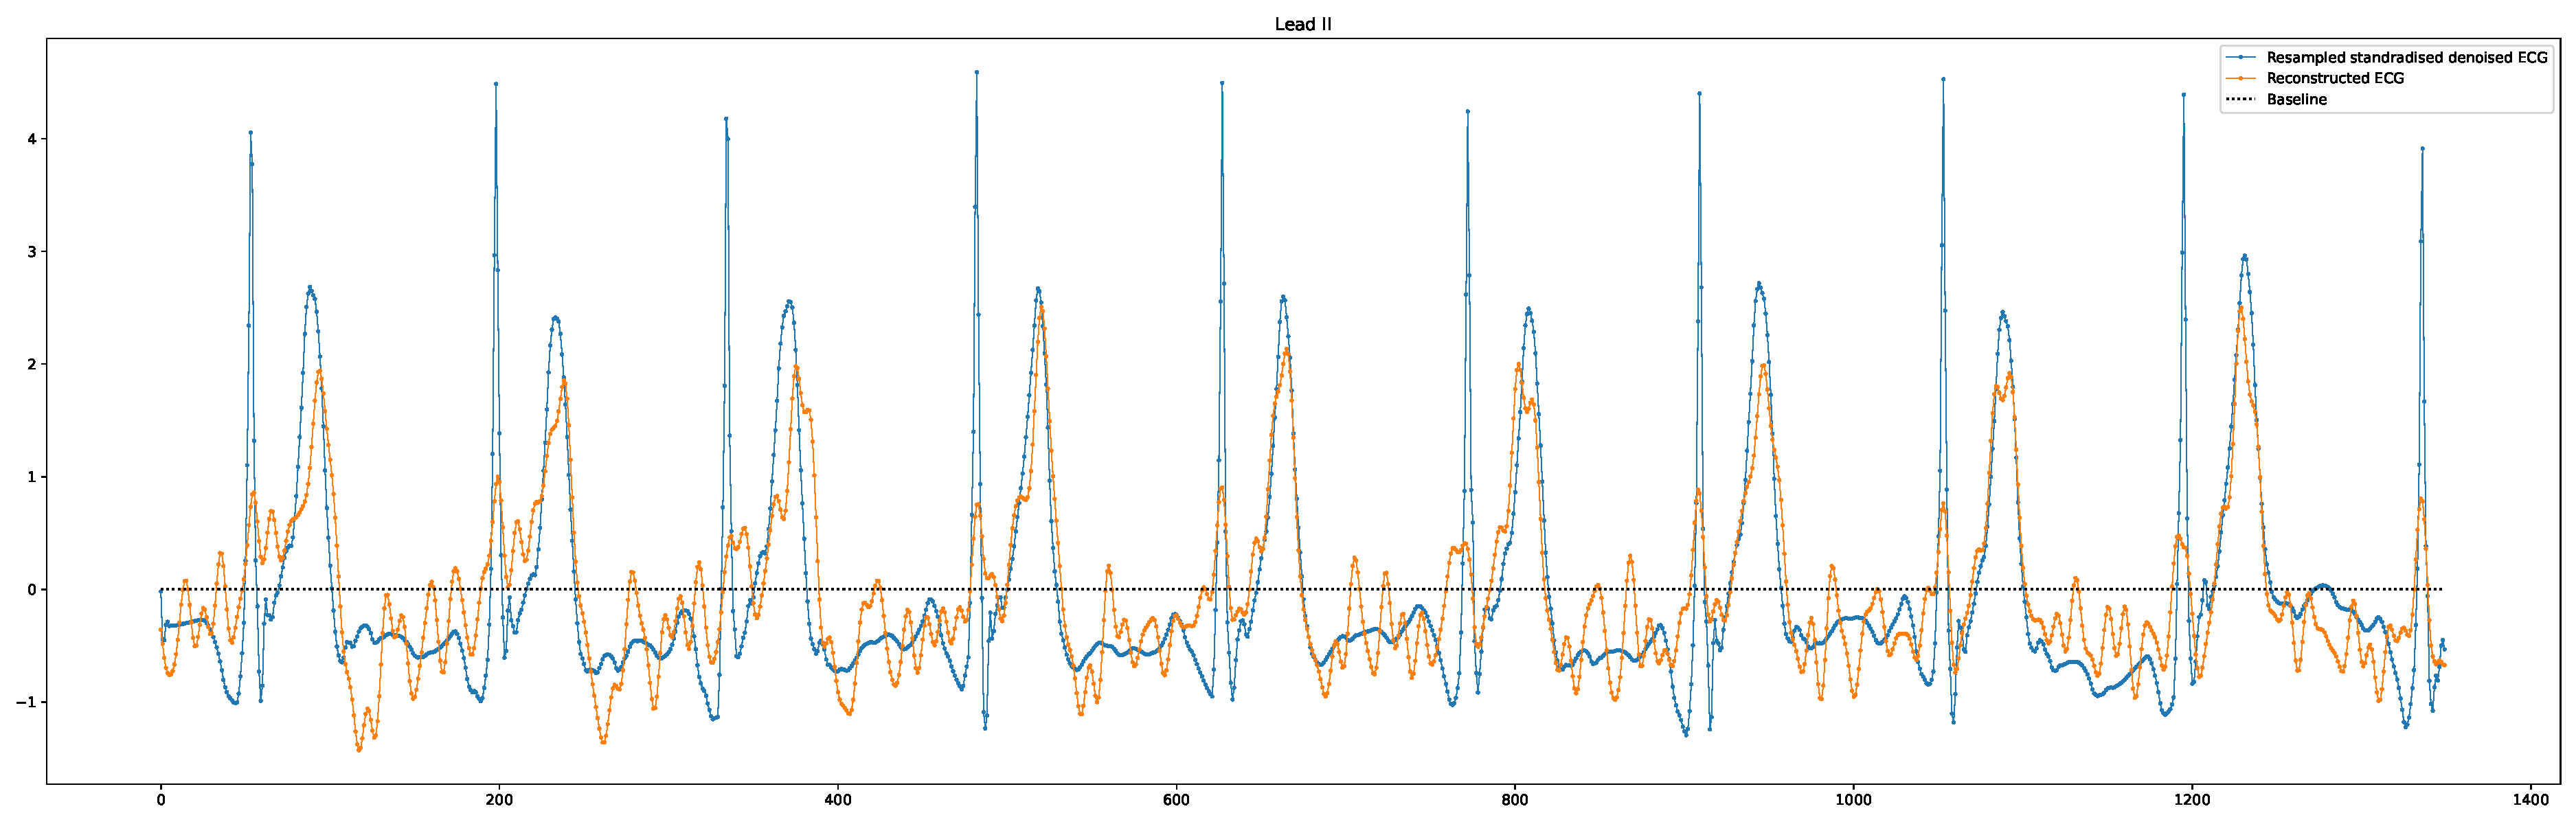
\includegraphics[width=1\linewidth]{images/r_peaks/resampled_standardised_denoised_ecg_reconstruction_m.pdf}
\caption{Resampled Lead II signal (blue), and the reconstruction (orange) of the same signal after applying PSMF to the 12 leads with rank $r = 3$, Fourier basis with $n = 3$ terms, and $100$ iterations.}
\label{fig:reconstr-ecg}
\end{figure}

\begin{figure}[H]
\centering
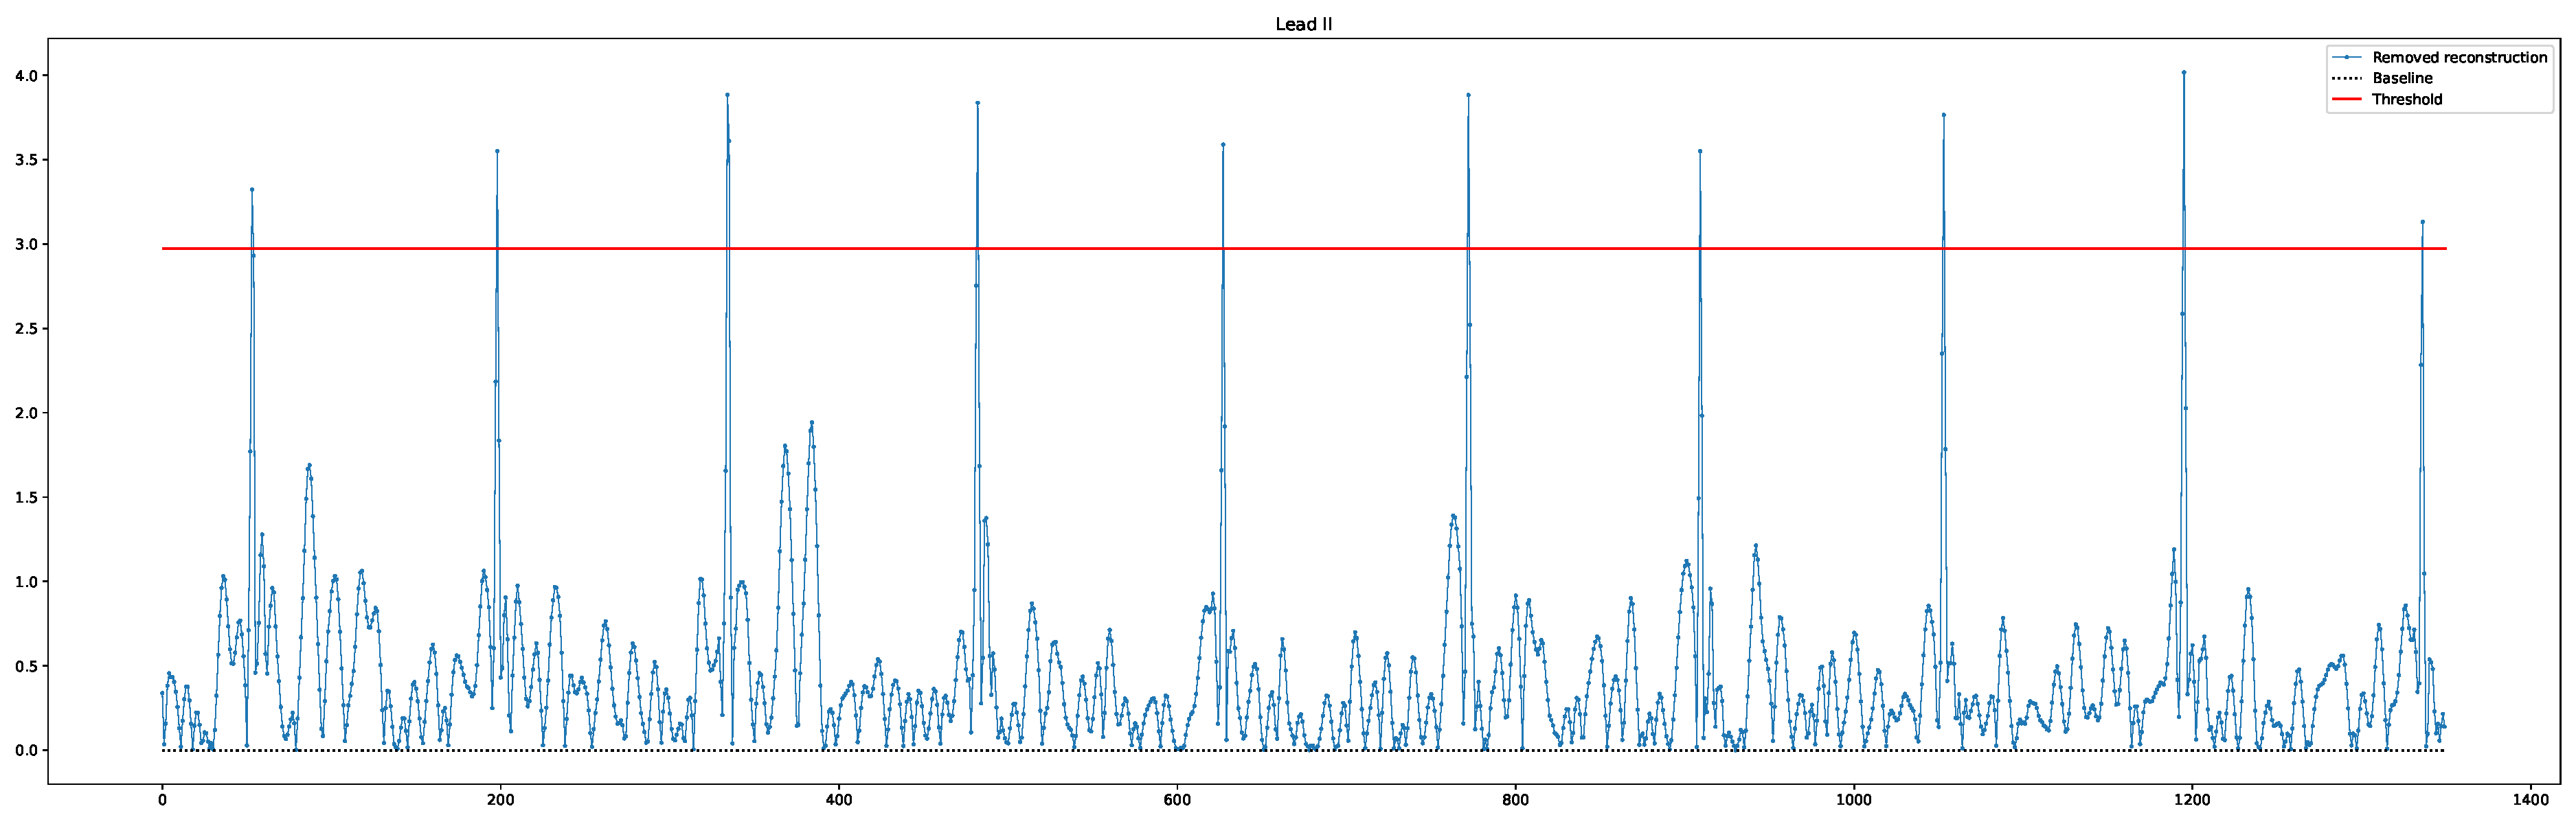
\includegraphics[width=1\linewidth]{images/r_peaks/resampled_standardised_denoised_ecg_rpeaks_algo_m.pdf}
\caption{Removed reconstruction from the modelled ECG signal (blue), and threshold (red) for isolating the R-peaks.}
\label{fig:diff-ecg}
\end{figure}

\begin{figure}[H]
\centering
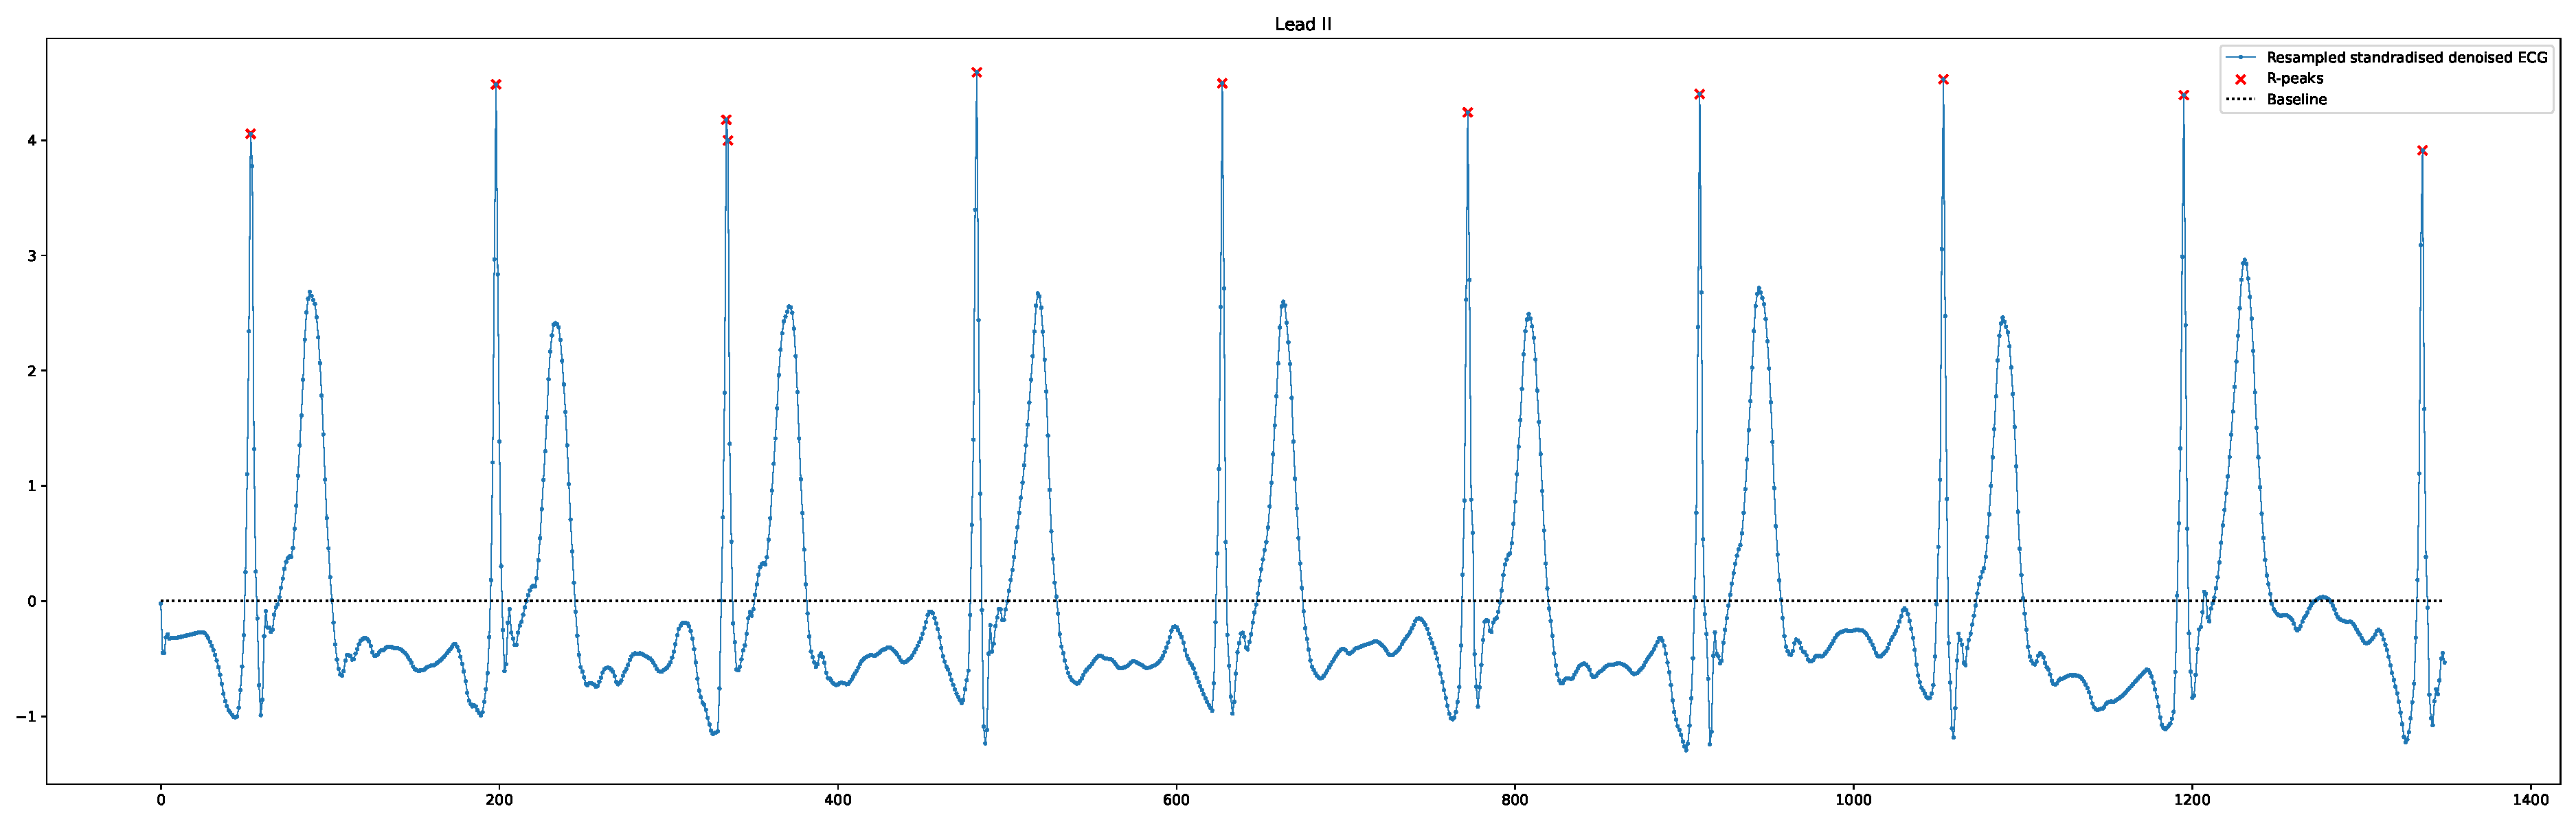
\includegraphics[width=1\linewidth]{images/r_peaks/resampled_standardised_denoised_ecg_rpeaks_m.pdf}
\caption{Detected R-peaks (red) in the resampled, standardised, denoised Lead II signal (blue).}
\label{fig:rpeaks-ecg}
\end{figure}

Full results, appendix - more?

\begin{figure}[H]
\centering
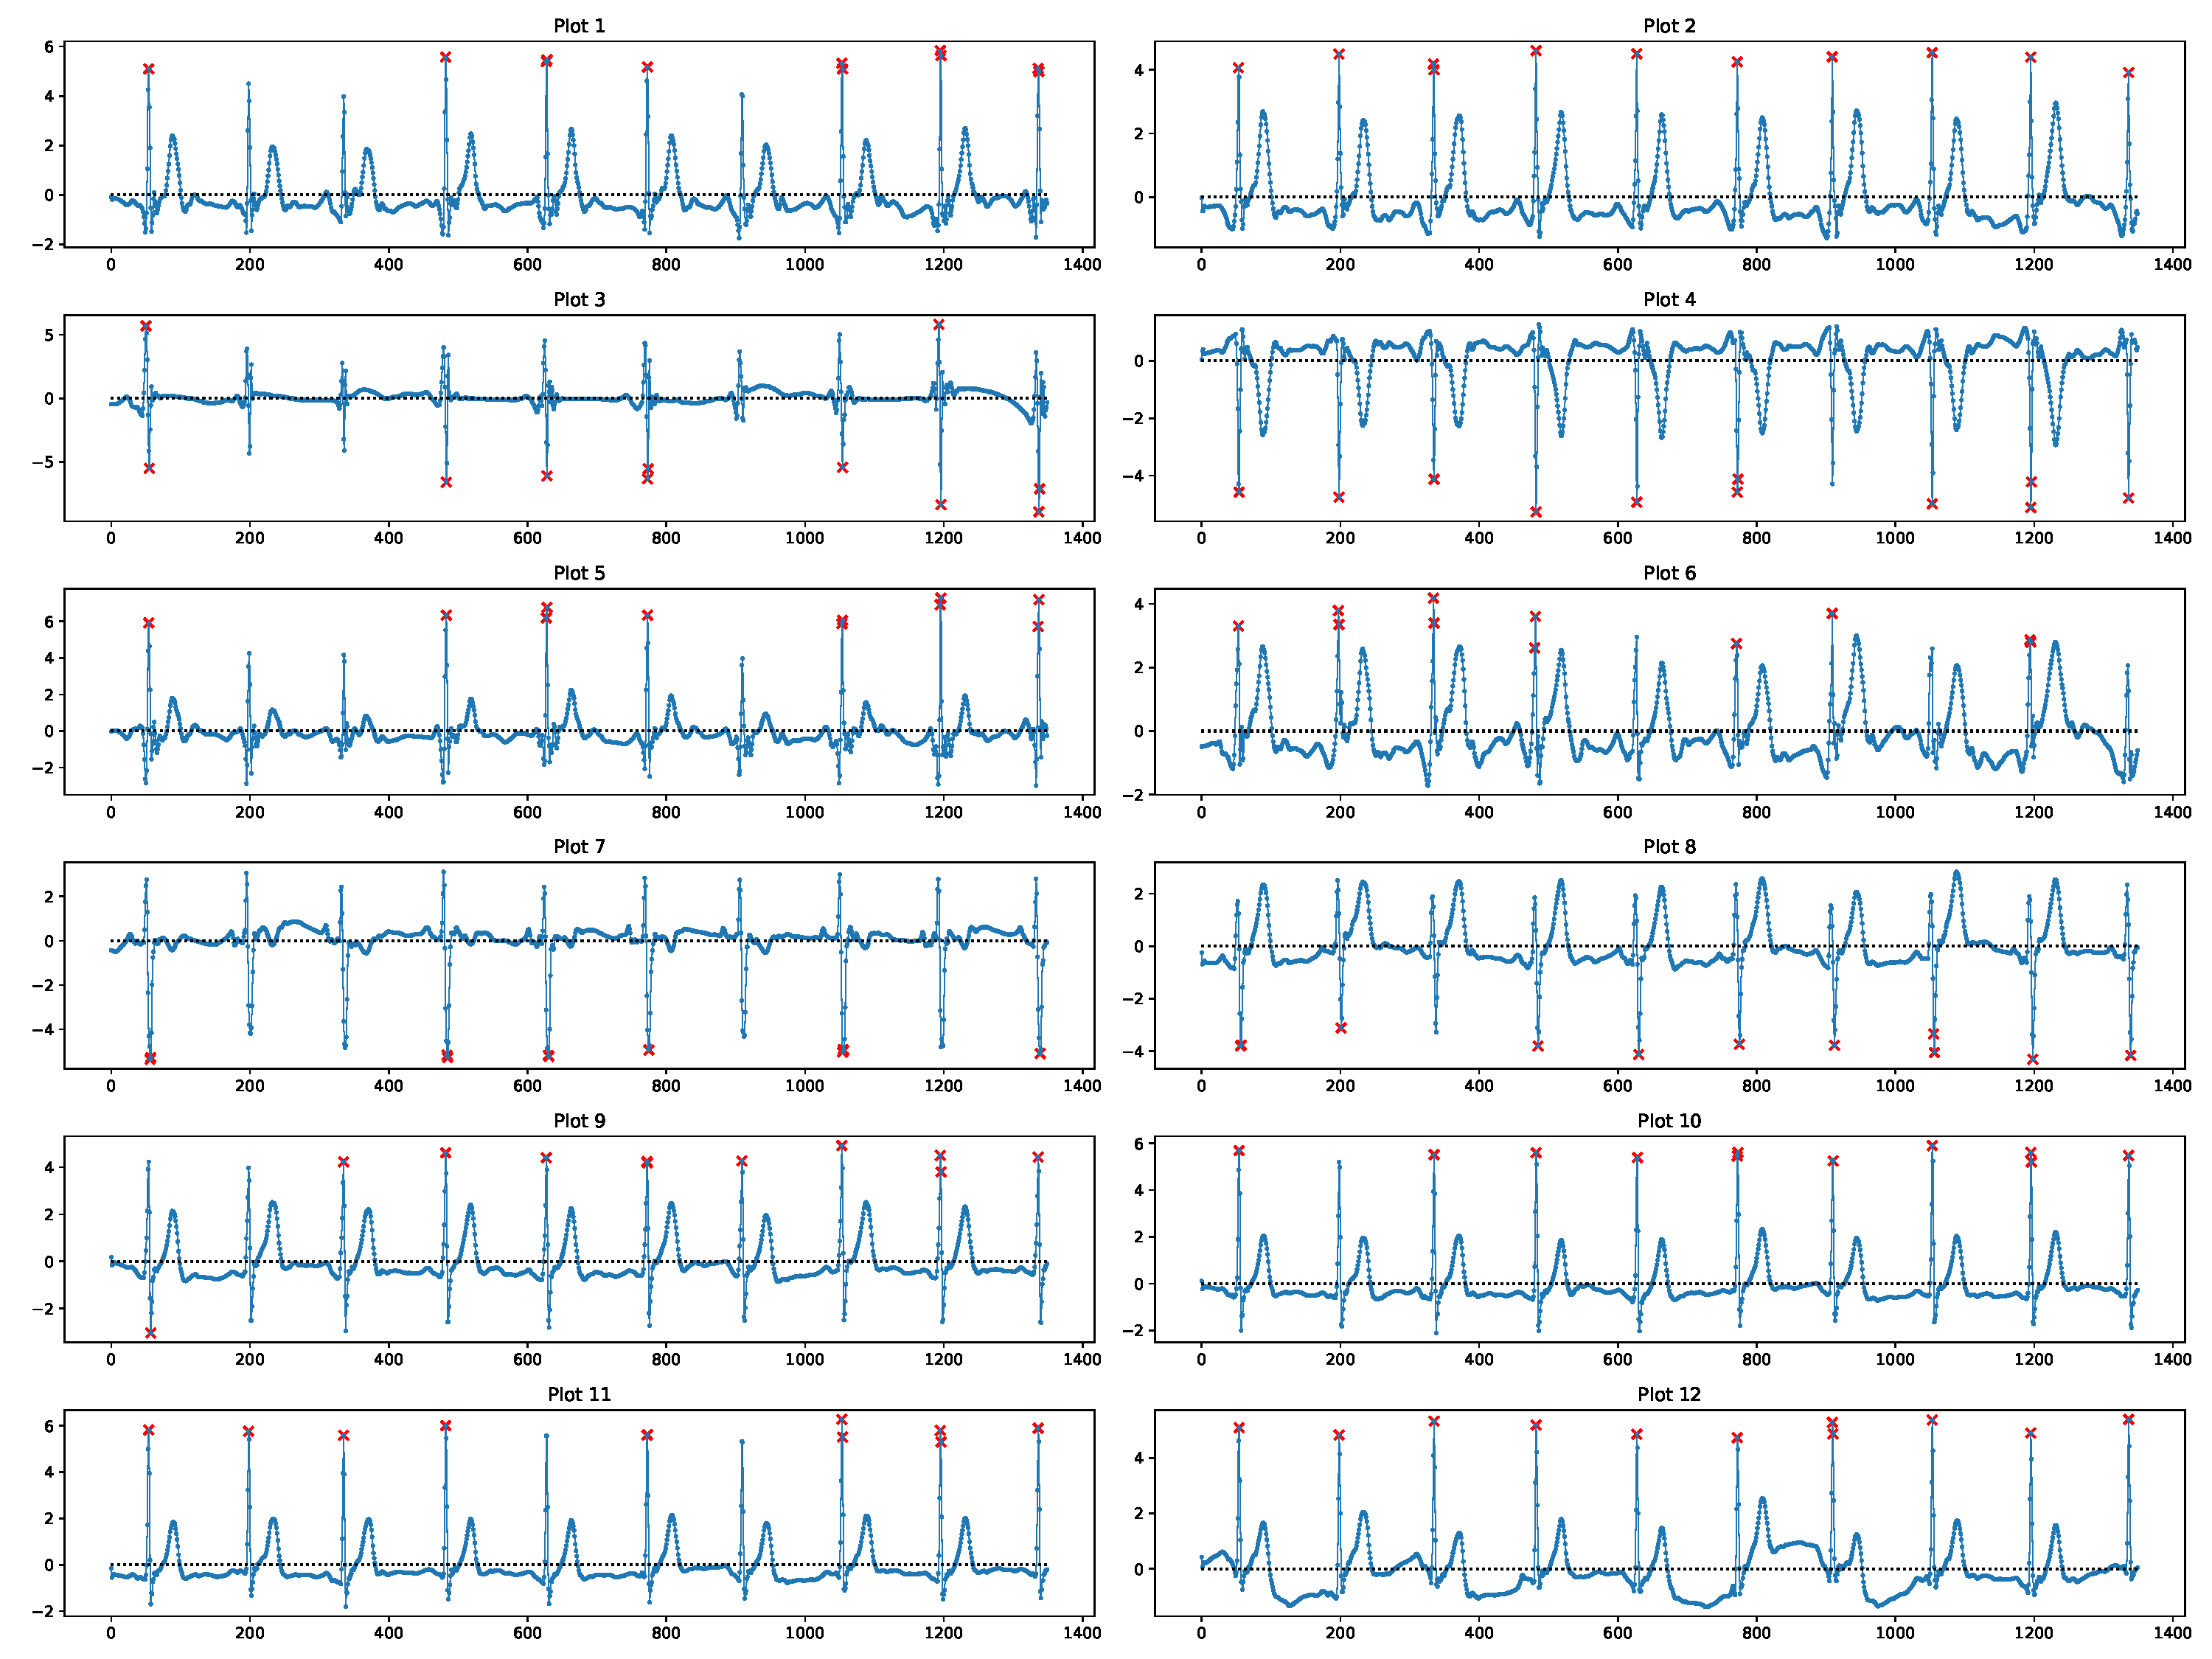
\includegraphics[width=1\linewidth]{images/r_peaks/rpeaks_full_m.pdf}
\caption{Detected R-peaks (red) in the resampled, standardised, denoised 12-Lead ECG signal (blue).}
\label{fig:rpeaks-ecg}
\end{figure}

\section{Forecasting}

TODO:

\begin{itemize}
    \item original data (5000) vs subsample (1500)
    \item smoothing vs no smoothing
    \item Fourier basis and number of terms, higher rank
    \item encountered issues, conclusions
    \item add figures for the basis, loss curves, forecast (show different experiments results)
\end{itemize}

\begin{figure}[H]
\begin{center}
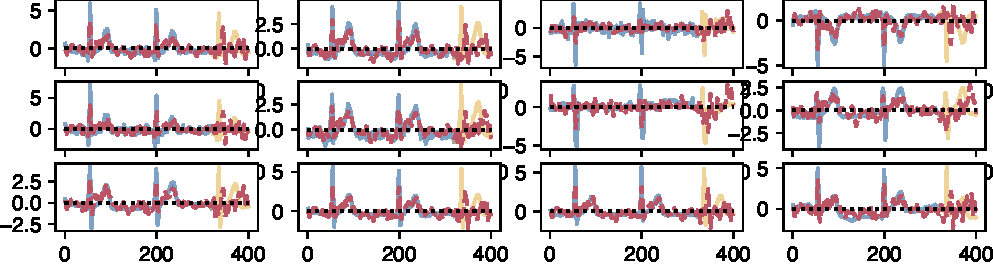
\includegraphics[scale=1]{images/periodic_fit_1500_6_6_150it.pdf}
\caption{My caption here}
\label{somelabelforreference}
\end{center}
\end{figure}

\begin{figure}[H]
\begin{center}
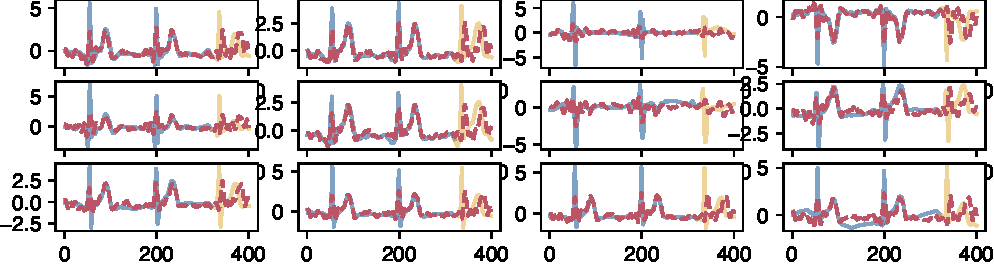
\includegraphics[scale=1]{images/forecast/periodic_fit.pdf}
\caption{rank 6, terms 3, 400 iterations, wavelet, standardised, 400 points out of 1500 resampled, 20\% test}
\label{forecast}
\end{center}
\end{figure}

\begin{figure}[H]
\begin{center}
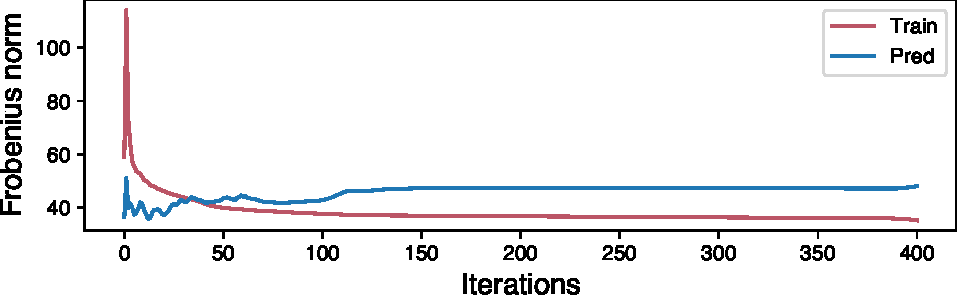
\includegraphics[scale=1]{images/forecast/periodic_cost.pdf}
\caption{rank 6, terms 3, 400 iterations, wavelet, standardised, 400 points out of 1500 resampled, 20\% test}
\label{loss}
\end{center}
\end{figure}

\begin{figure}[H]
\begin{center}
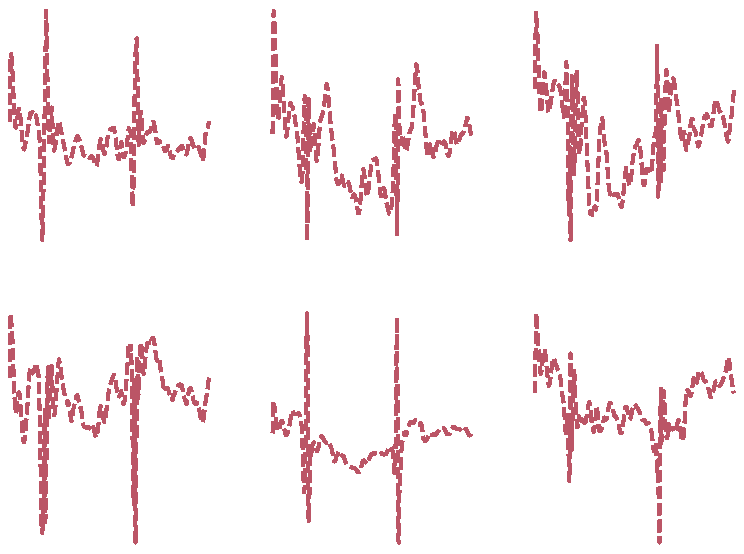
\includegraphics[scale=1]{images/forecast/periodic_bases.pdf}
\caption{rank 6, terms 3, 400 iterations, wavelet, standardised, 400 points out of 1500 resampled, 20\% test}
\label{bases}
\end{center}
\end{figure}

\chapter{Conclusion}

TODO: summarise results

\section{Future work}

TODO:
\begin{itemize}
    \item More complex model to better suit the complexity of the ECG data
    \item Better computational efficiency
\end{itemize}

Why modelling ecg is usefu? SPecifically normal sinus rhythm.

Why detecting ECG is useful?

\clearpage
 %% reset page counter and start appendix pages with A
\pagenumbering{arabic}
\renewcommand*{\thepage}{A\arabic{page}}

%% Appendix goes here
\appendix

\chapter{Missing Data Imputation Results}

Full results of testing on the $20\%$, $30\%$, and $40\%$ missing data with both $r = 3$ and $r = 10$.

\section{PSMF}

\subsection{$r = 3$}

\begin{figure}[H]
\centering
% First row
\begin{minipage}{0.4\linewidth}
    \centering
    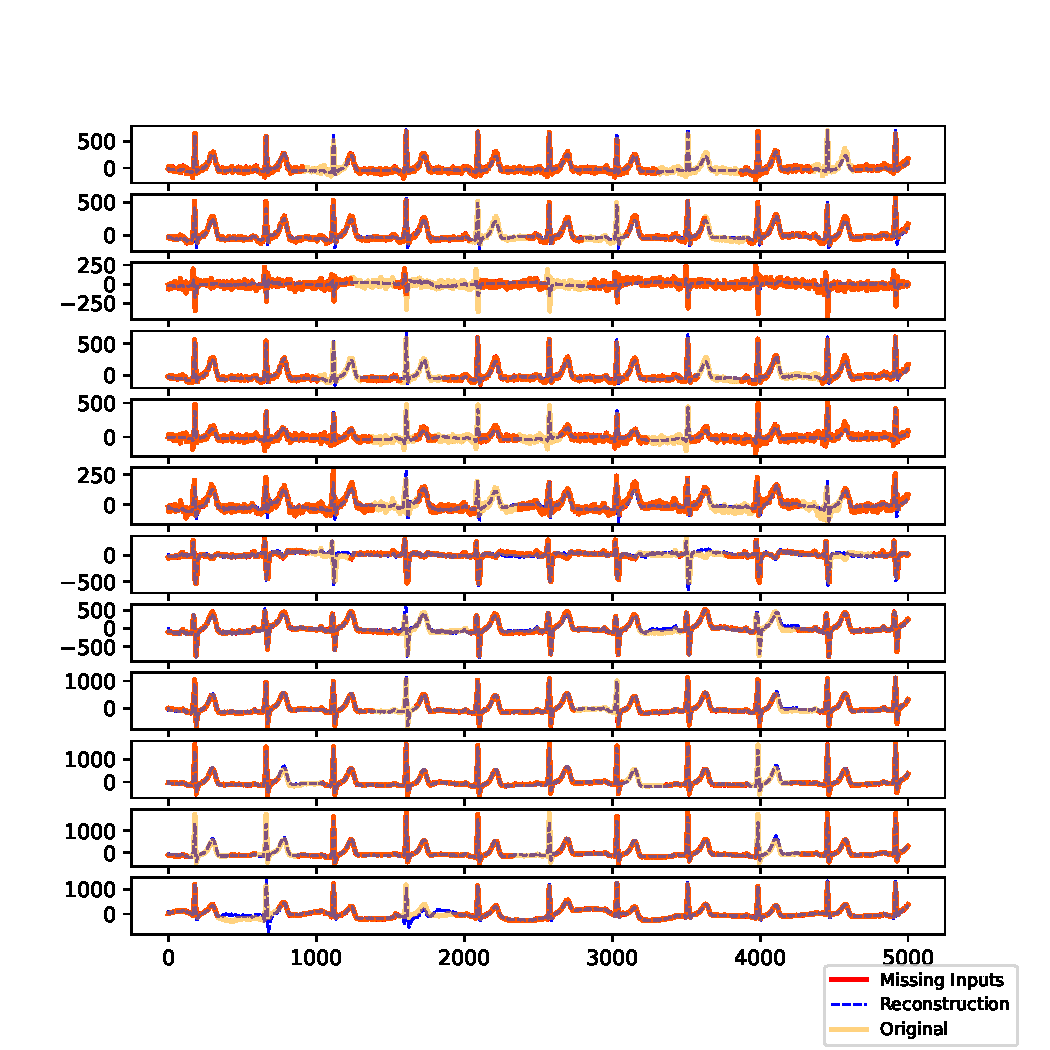
\includegraphics[width=\linewidth]{images/missing/psmf_output_20_3.pdf}
    \caption{$20\%$ missing data.}
\end{minipage}%
\hspace{0.05\linewidth}
\begin{minipage}{0.4\linewidth}
    \centering
    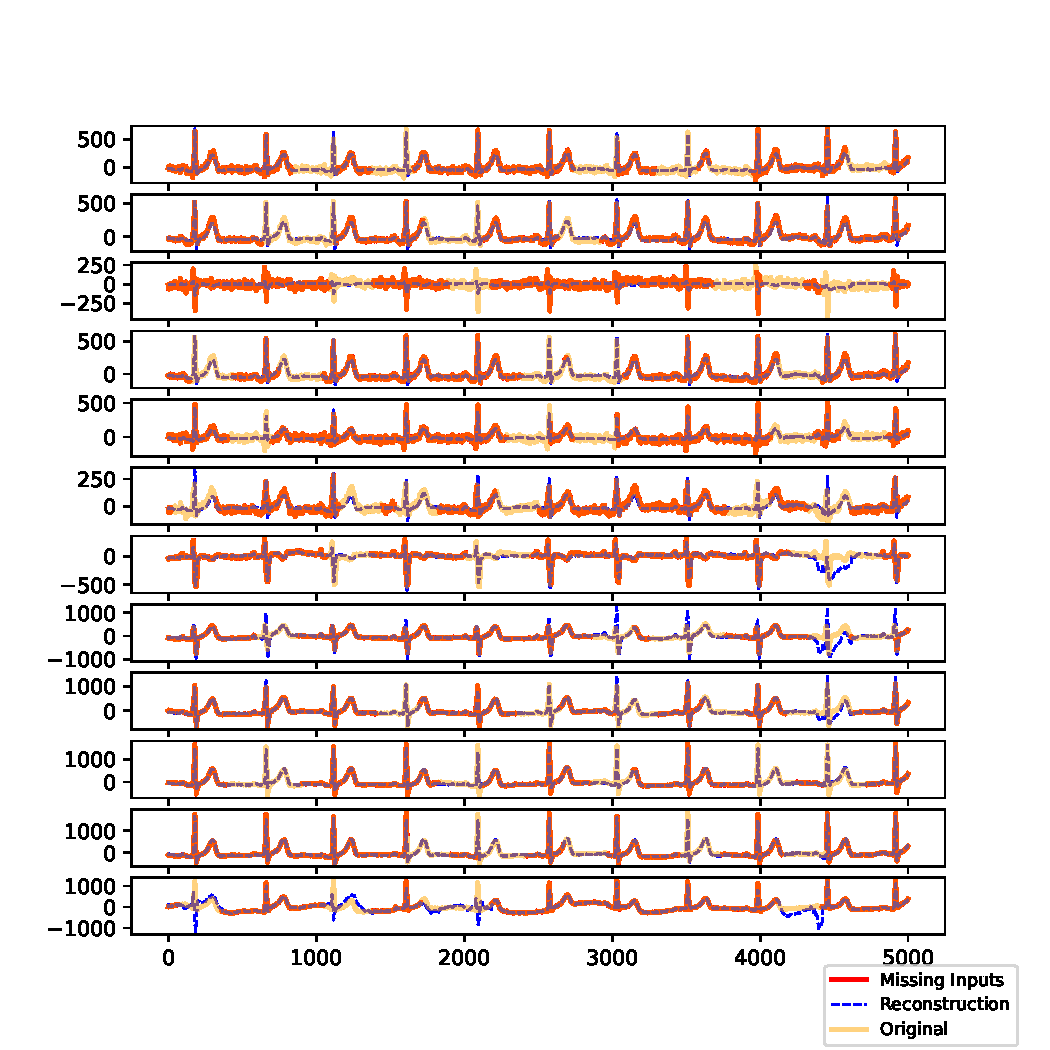
\includegraphics[width=\linewidth]{images/missing/psmf_output_30_3.pdf}
    \caption{$30\%$ missing data.}
\end{minipage}

\vspace{1em} % Adjust vertical space between the rows if necessary

% Second row
\begin{minipage}{0.4\linewidth}
    \centering
    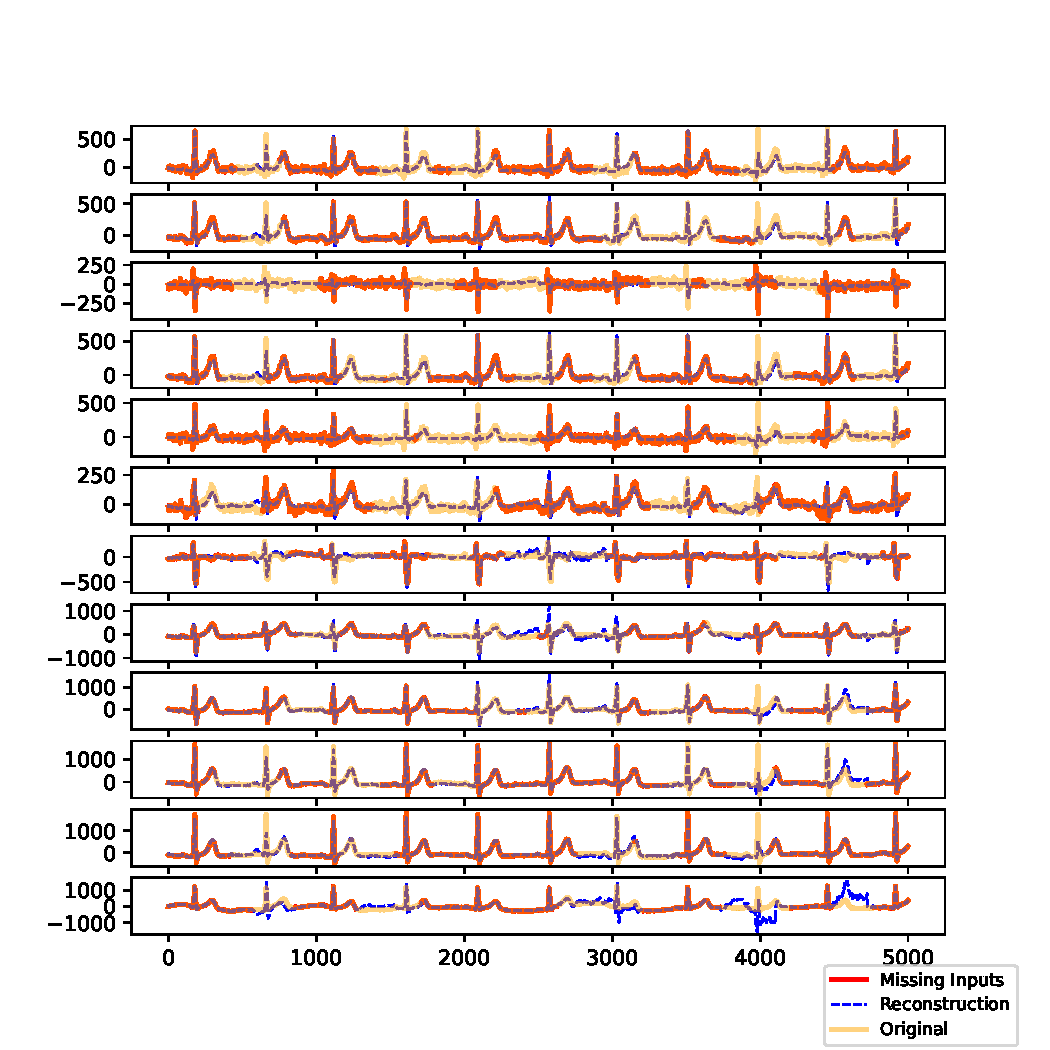
\includegraphics[width=\linewidth]{images/missing/psmf_output_40_3.pdf}
    \caption{$40\%$ missing data.}
\end{minipage}
\end{figure}

\subsection{$r = 10$}

\begin{figure}[H]
\centering
% First row
\begin{minipage}{0.4\linewidth}
    \centering
    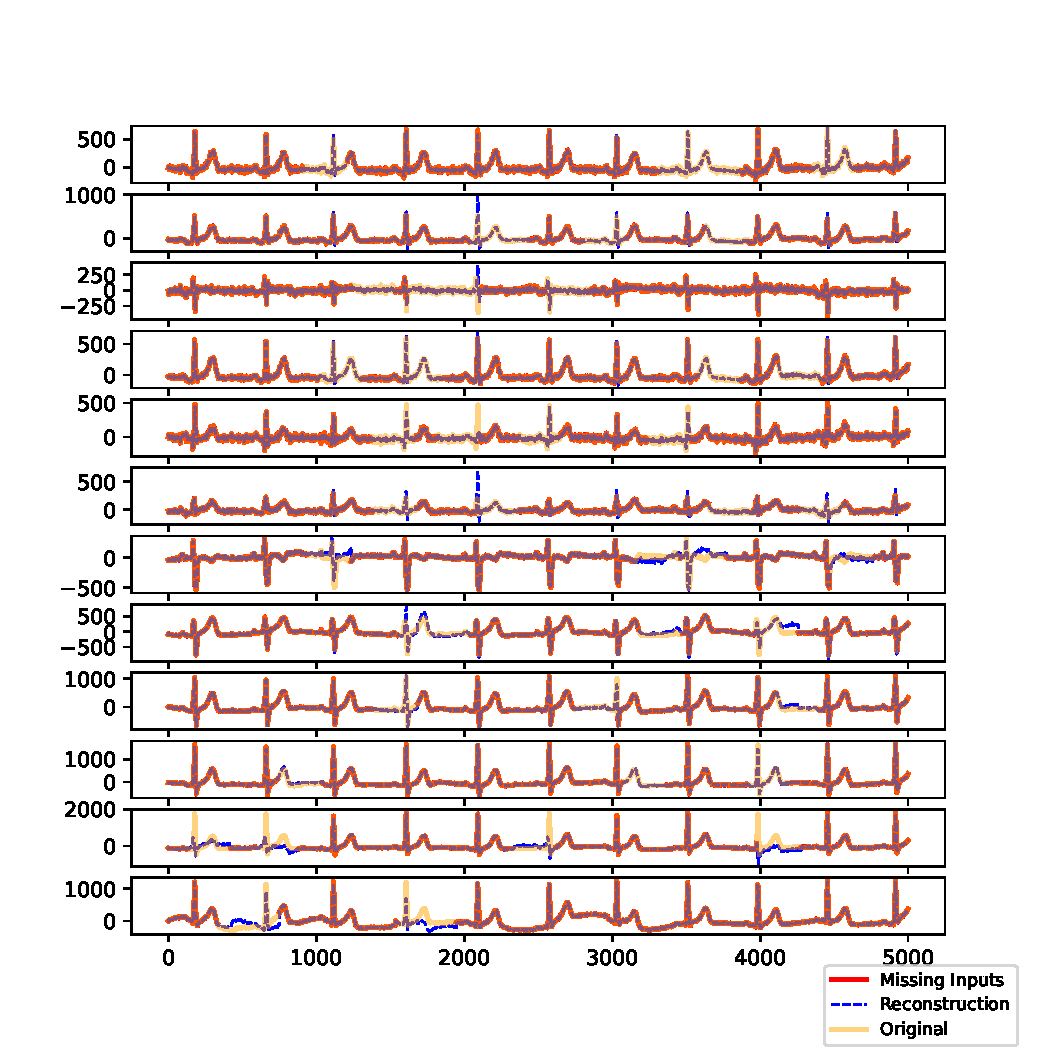
\includegraphics[width=\linewidth]{images/missing/psmf_output_20_10.pdf}
    \caption{$20\%$ missing data.}
\end{minipage}%
\hspace{0.05\linewidth}
\begin{minipage}{0.4\linewidth}
    \centering
    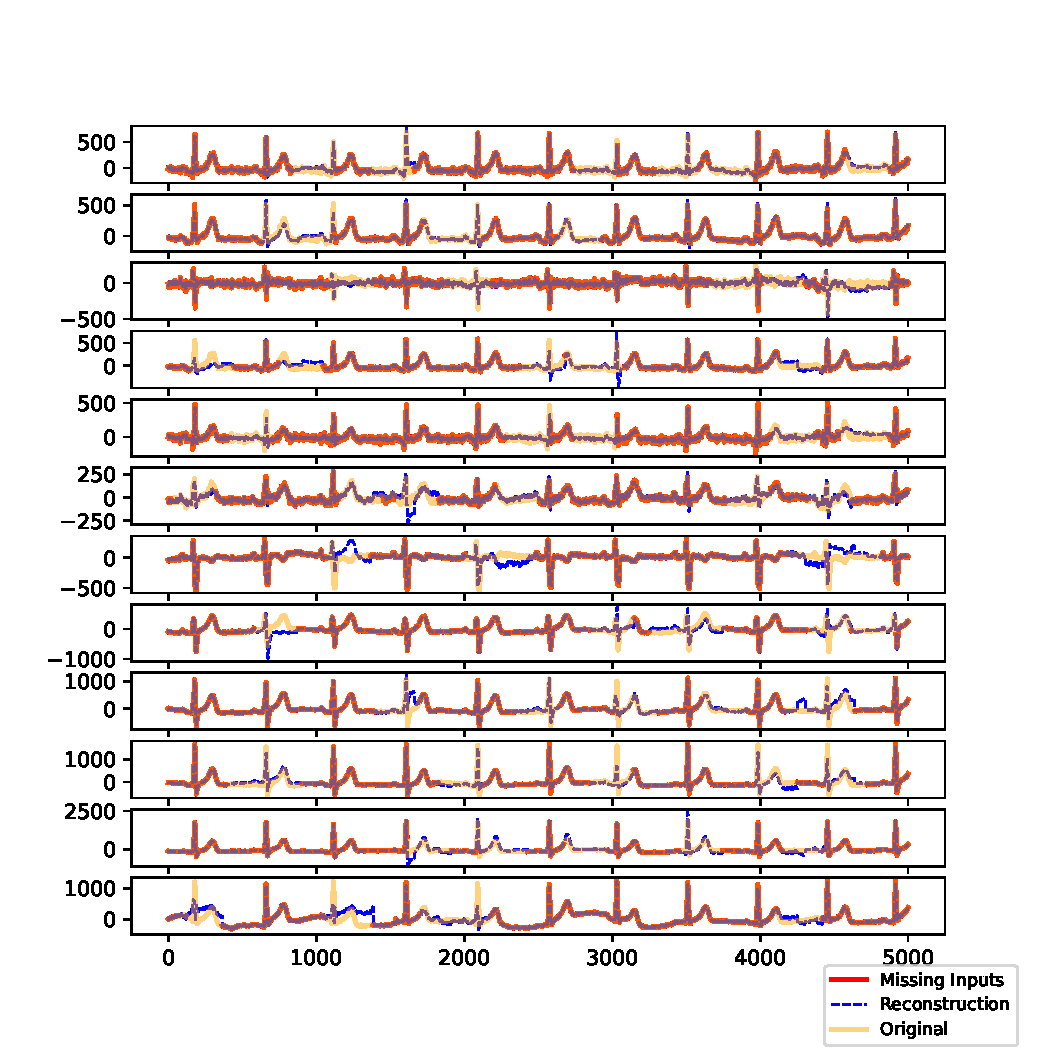
\includegraphics[width=\linewidth]{images/missing/psmf_output_30_10.pdf}
    \caption{$30\%$ missing data.}
\end{minipage}

\vspace{1em} % Adjust vertical space between the rows if necessary

% Second row
\begin{minipage}{0.4\linewidth}
    \centering
    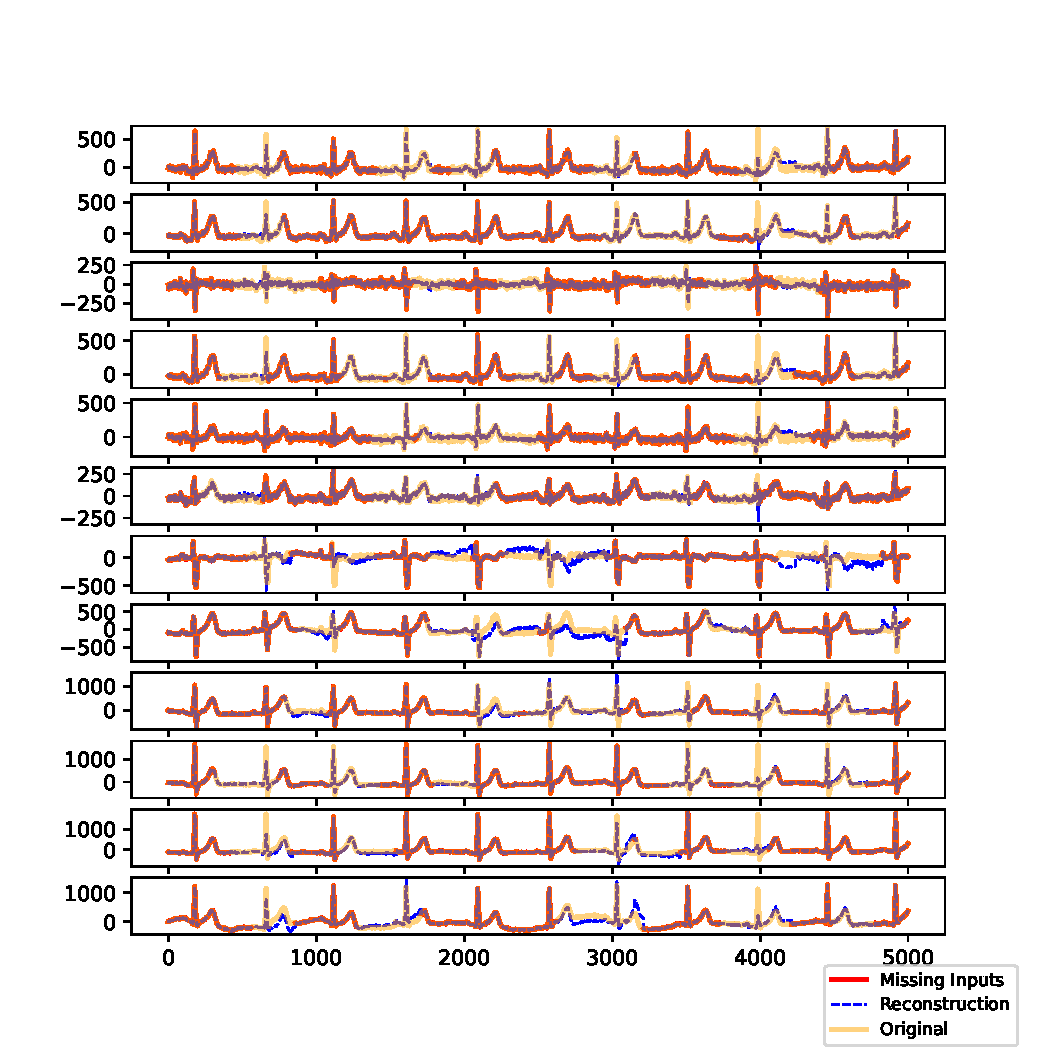
\includegraphics[width=\linewidth]{images/missing/psmf_output_40_10.pdf}
    \caption{$40\%$ missing data.}
\end{minipage}
\end{figure}

\section{rPSMF}

\subsection{$r = 3$}

\begin{figure}[H]
\centering
% First row
\begin{minipage}{0.4\linewidth}
    \centering
    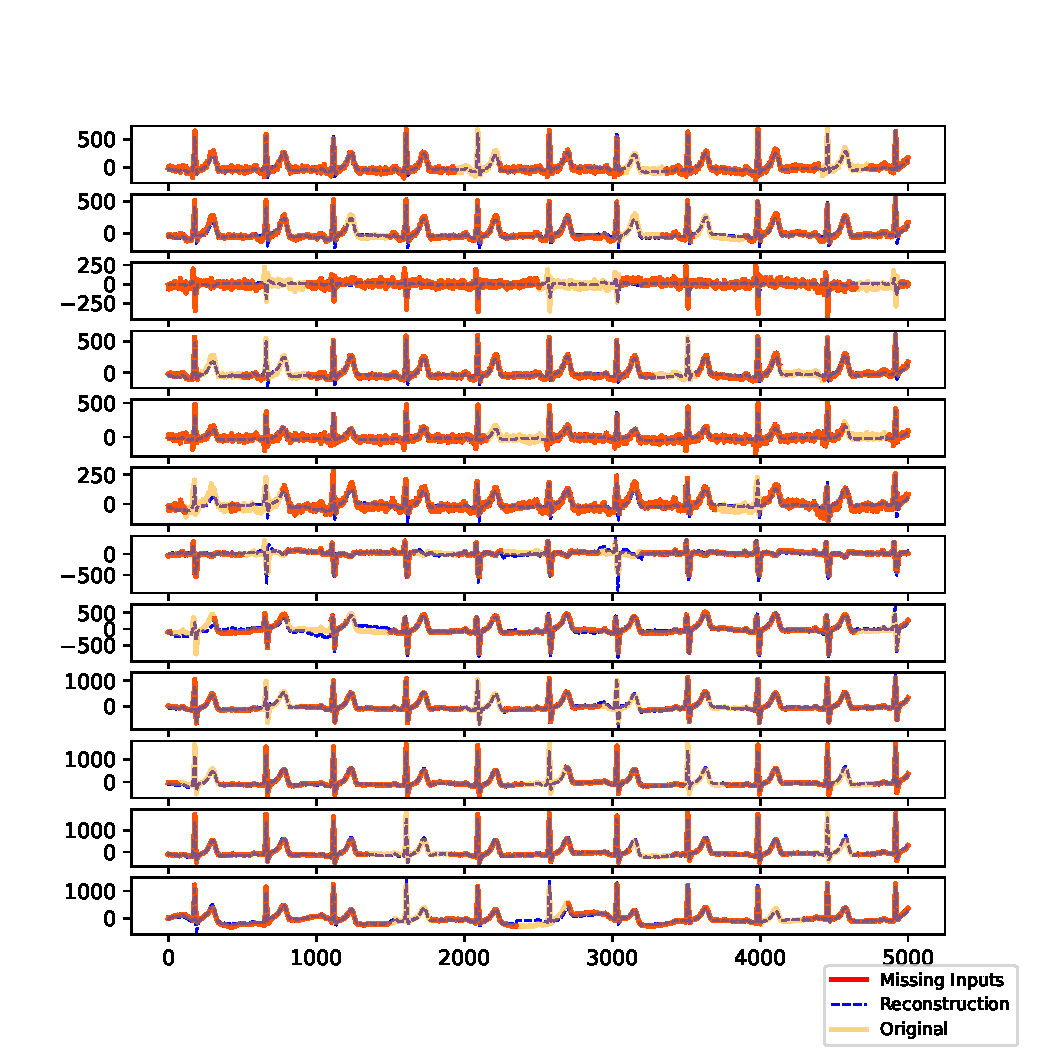
\includegraphics[width=\linewidth]{images/missing/rpsmf_output_20_3.pdf}
    \caption{$20\%$ missing data.}
\end{minipage}%
\hspace{0.05\linewidth}
\begin{minipage}{0.4\linewidth}
    \centering
    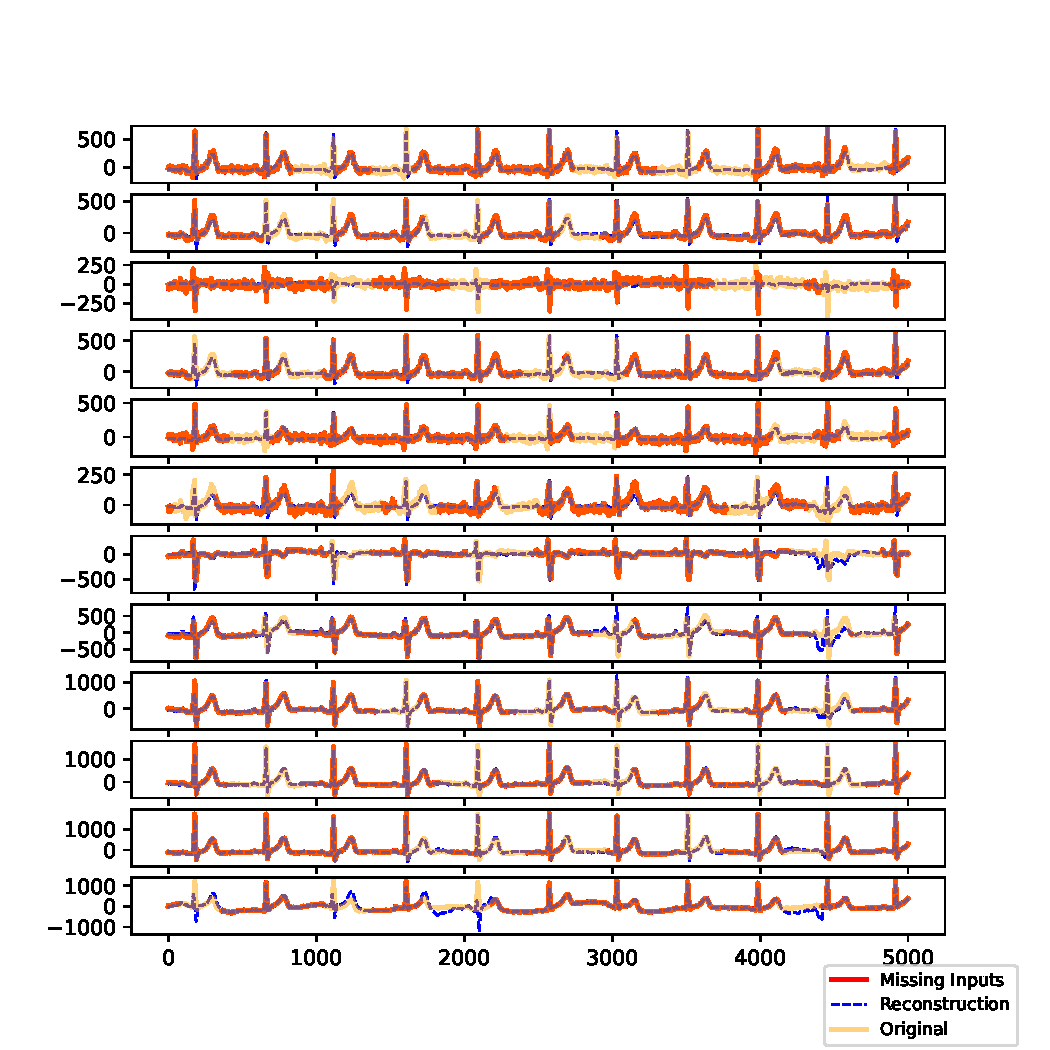
\includegraphics[width=\linewidth]{images/missing/rpsmf_output_30_3.pdf}
    \caption{$30\%$ missing data.}
\end{minipage}

\vspace{1em} % Adjust vertical space between the rows if necessary

% Second row
\begin{minipage}{0.4\linewidth}
    \centering
    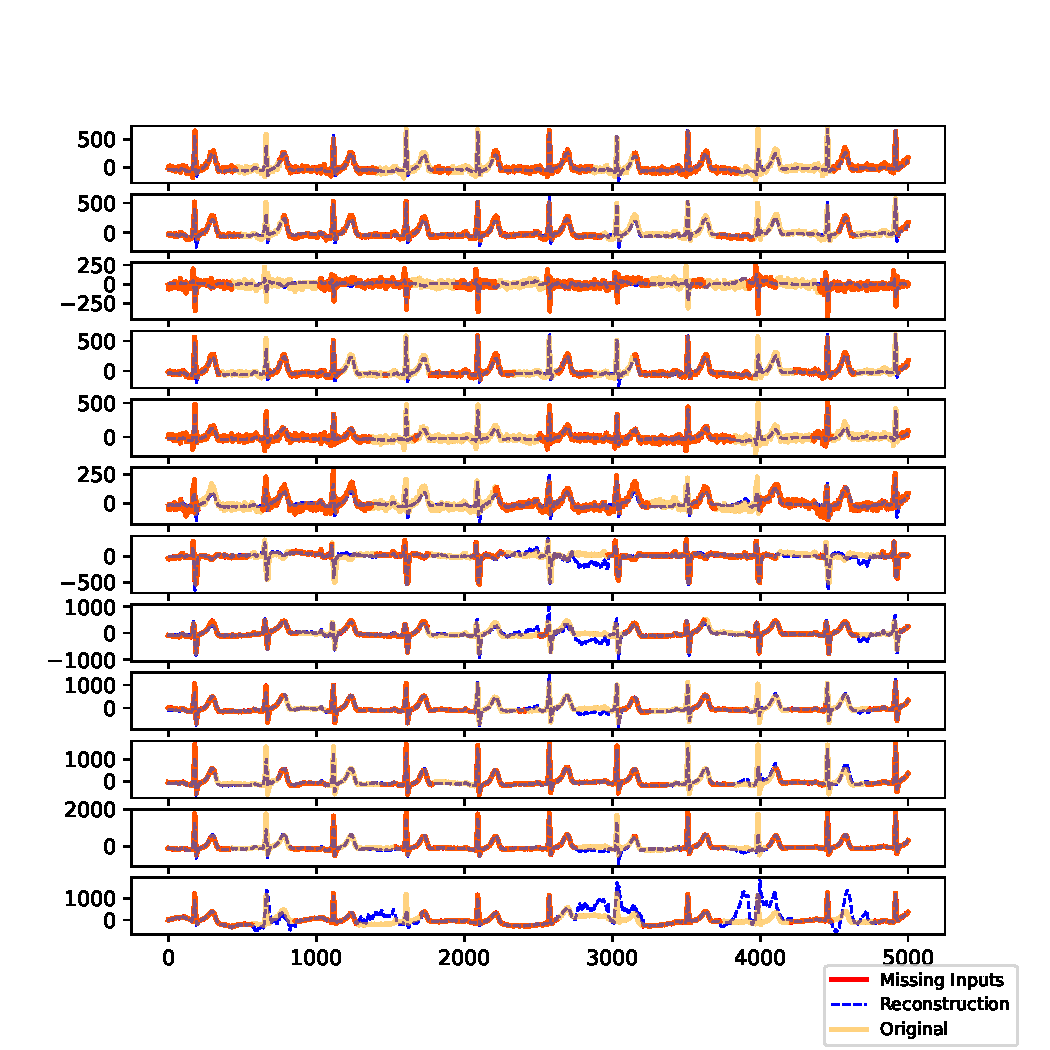
\includegraphics[width=\linewidth]{images/missing/rpsmf_output_40_3.pdf}
    \caption{$40\%$ missing data.}
\end{minipage}
\end{figure}

\subsection{$r = 10$}

\begin{figure}[H]
\centering
% First row
\begin{minipage}{0.4\linewidth}
    \centering
    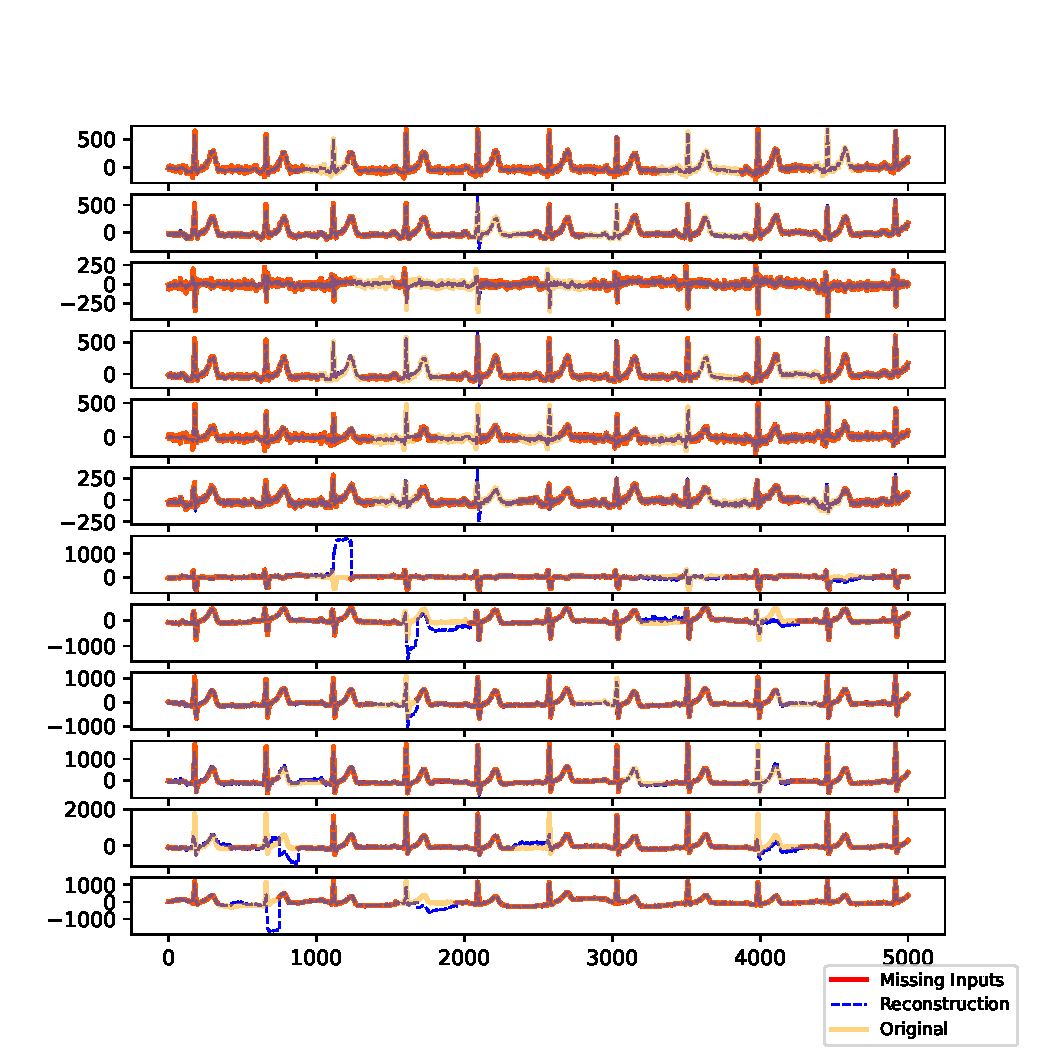
\includegraphics[width=\linewidth]{images/missing/rpsmf_output_20_10.pdf}
    \caption{$20\%$ missing data.}
\end{minipage}%
\hspace{0.05\linewidth}
\begin{minipage}{0.4\linewidth}
    \centering
    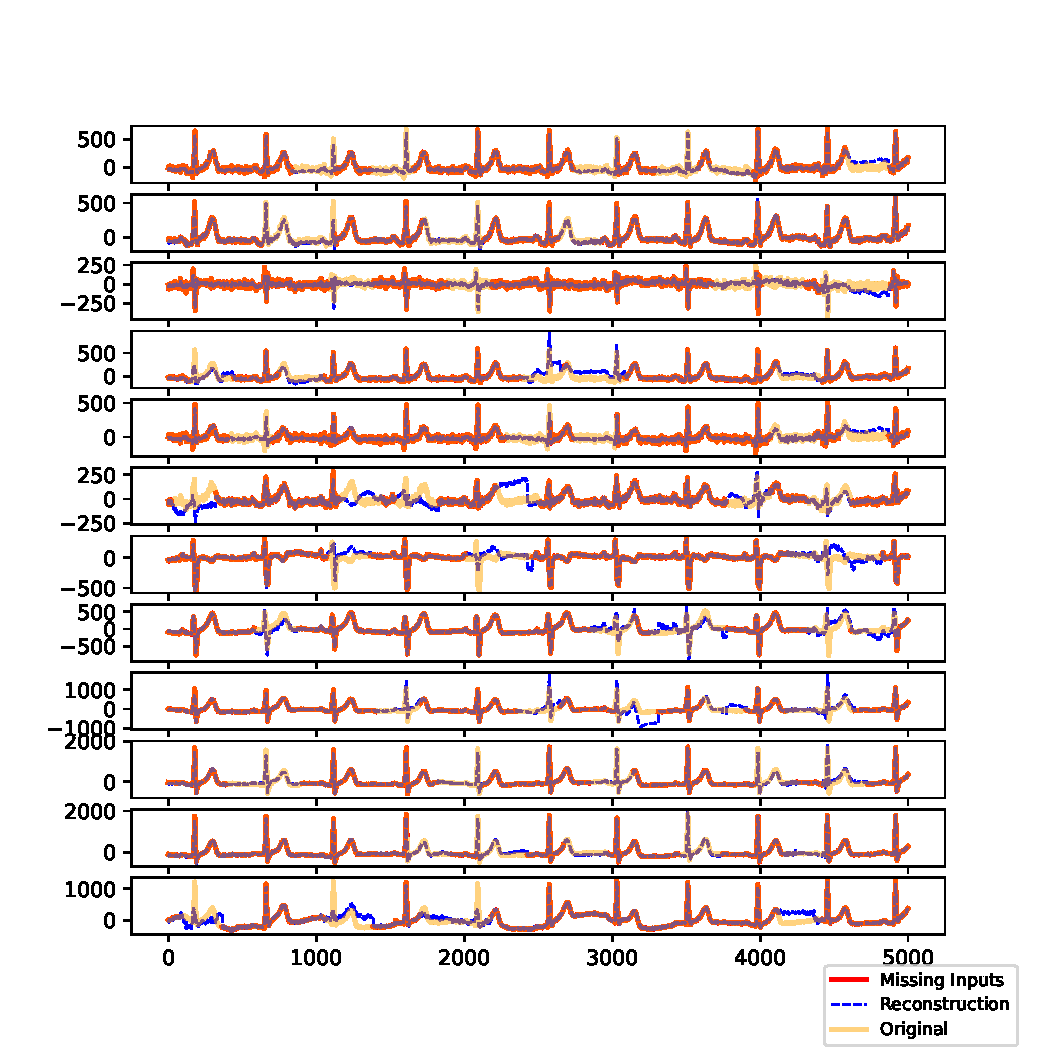
\includegraphics[width=\linewidth]{images/missing/rpsmf_output_30_10.pdf}
    \caption{$30\%$ missing data.}
\end{minipage}

\vspace{1em} % Adjust vertical space between the rows if necessary

% Second row
\begin{minipage}{0.4\linewidth}
    \centering
    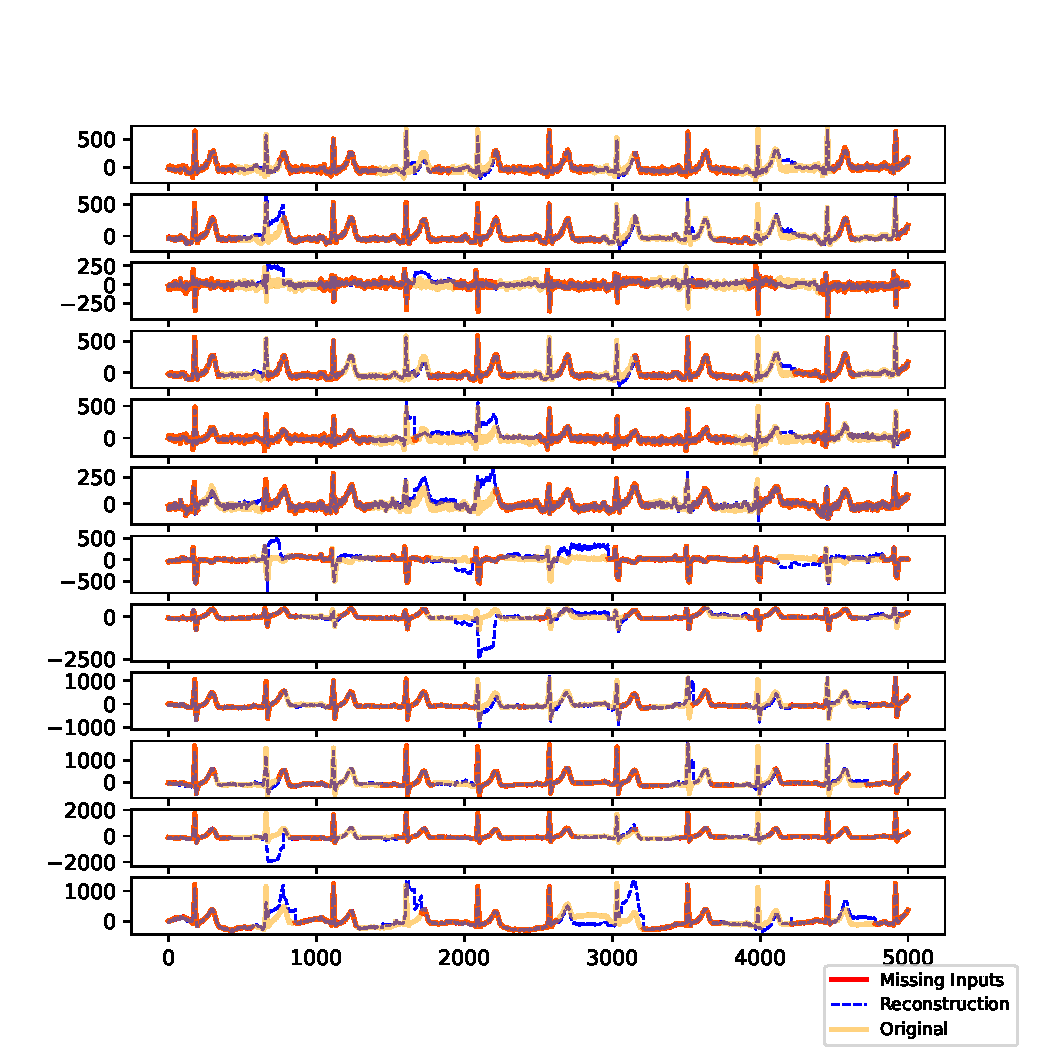
\includegraphics[width=\linewidth]{images/missing/rpsmf_output_40_10.pdf}
    \caption{$40\%$ missing data.}
\end{minipage}
\end{figure}

\section{MLE-SMF}

\subsection{$r = 3$}

\begin{figure}[H]
\centering
% First row
\begin{minipage}{0.4\linewidth}
    \centering
    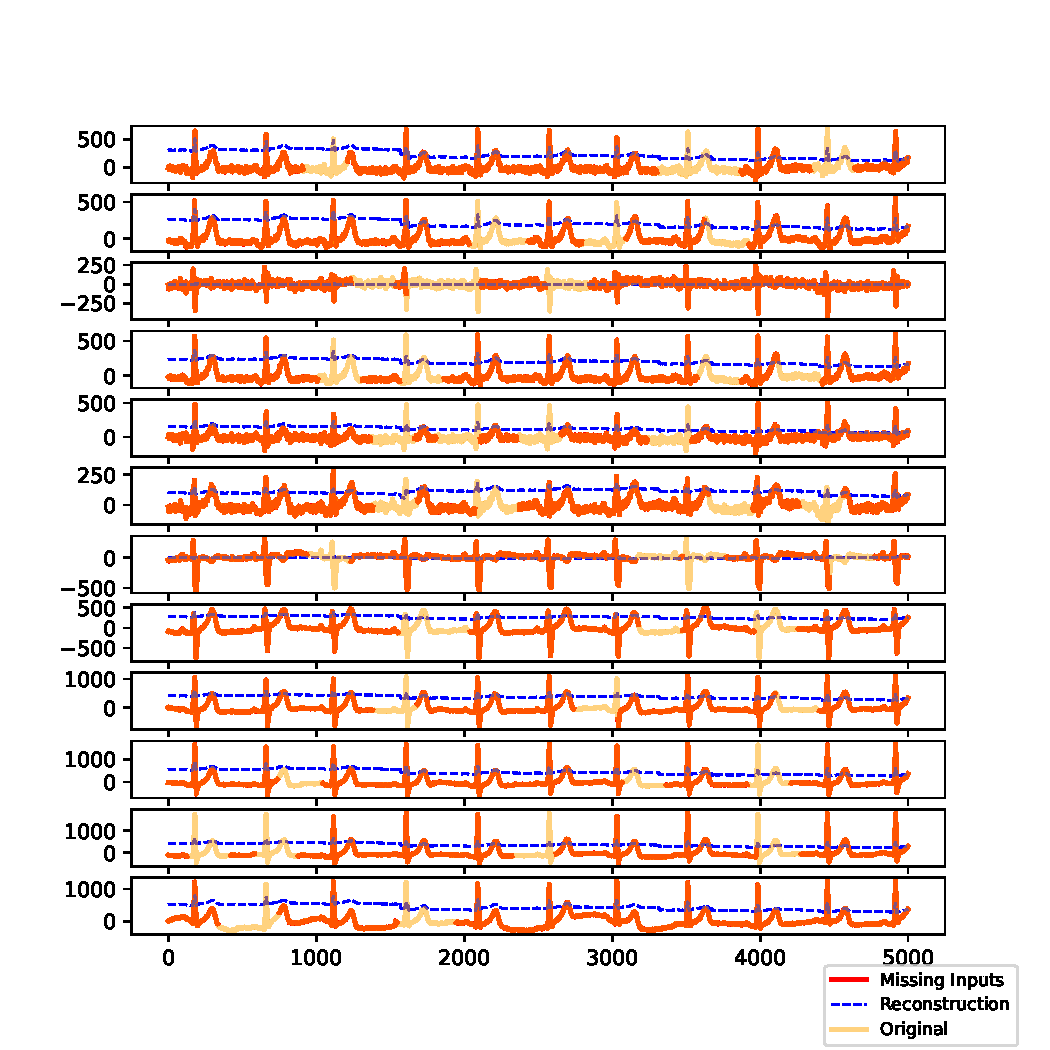
\includegraphics[width=\linewidth]{images/missing/mlesmf_output_20_3.pdf}
    \caption{$20\%$ missing data.}
\end{minipage}%
\hspace{0.05\linewidth}
\begin{minipage}{0.4\linewidth}
    \centering
    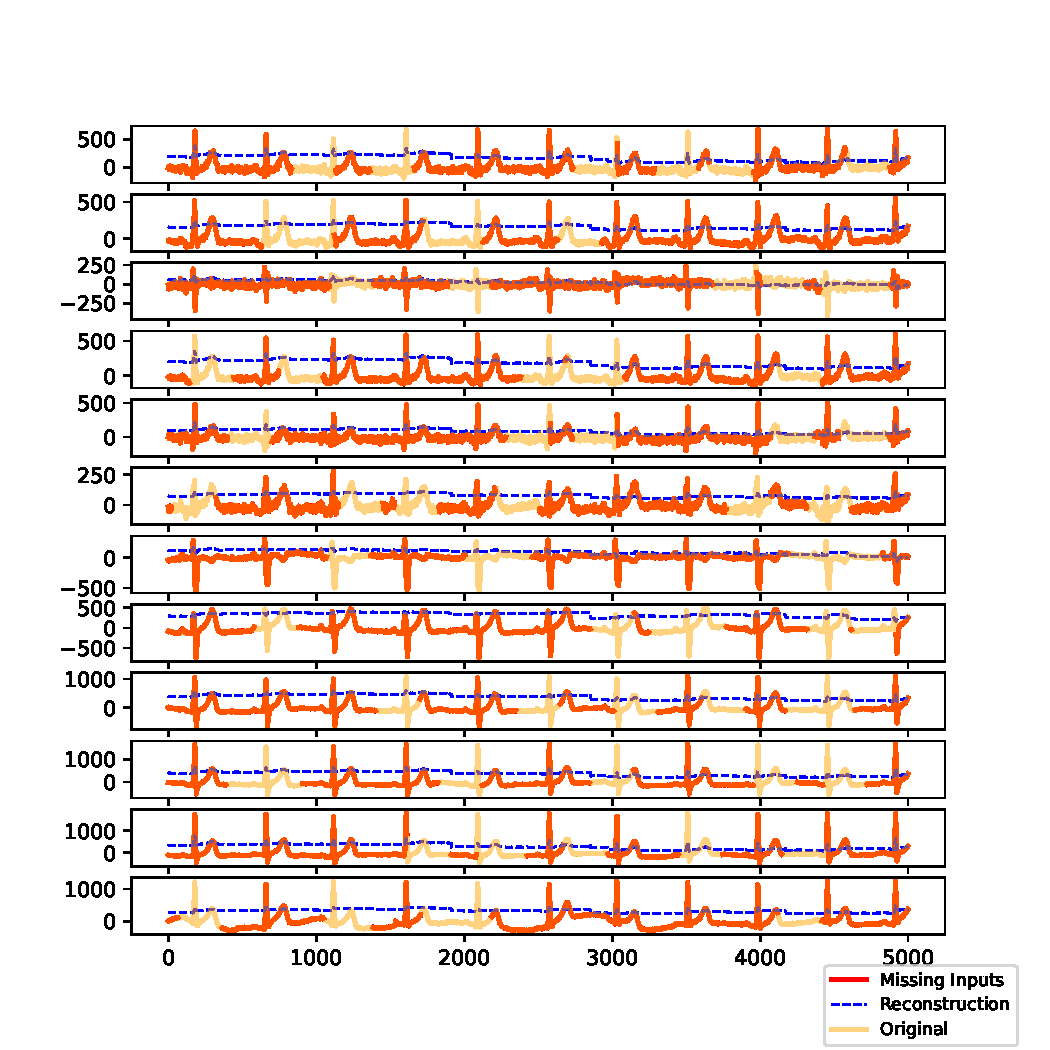
\includegraphics[width=\linewidth]{images/missing/mlesmf_output_30_3.pdf}
    \caption{$30\%$ missing data.}
\end{minipage}

\vspace{1em} % Adjust vertical space between the rows if necessary

% Second row
\begin{minipage}{0.4\linewidth}
    \centering
    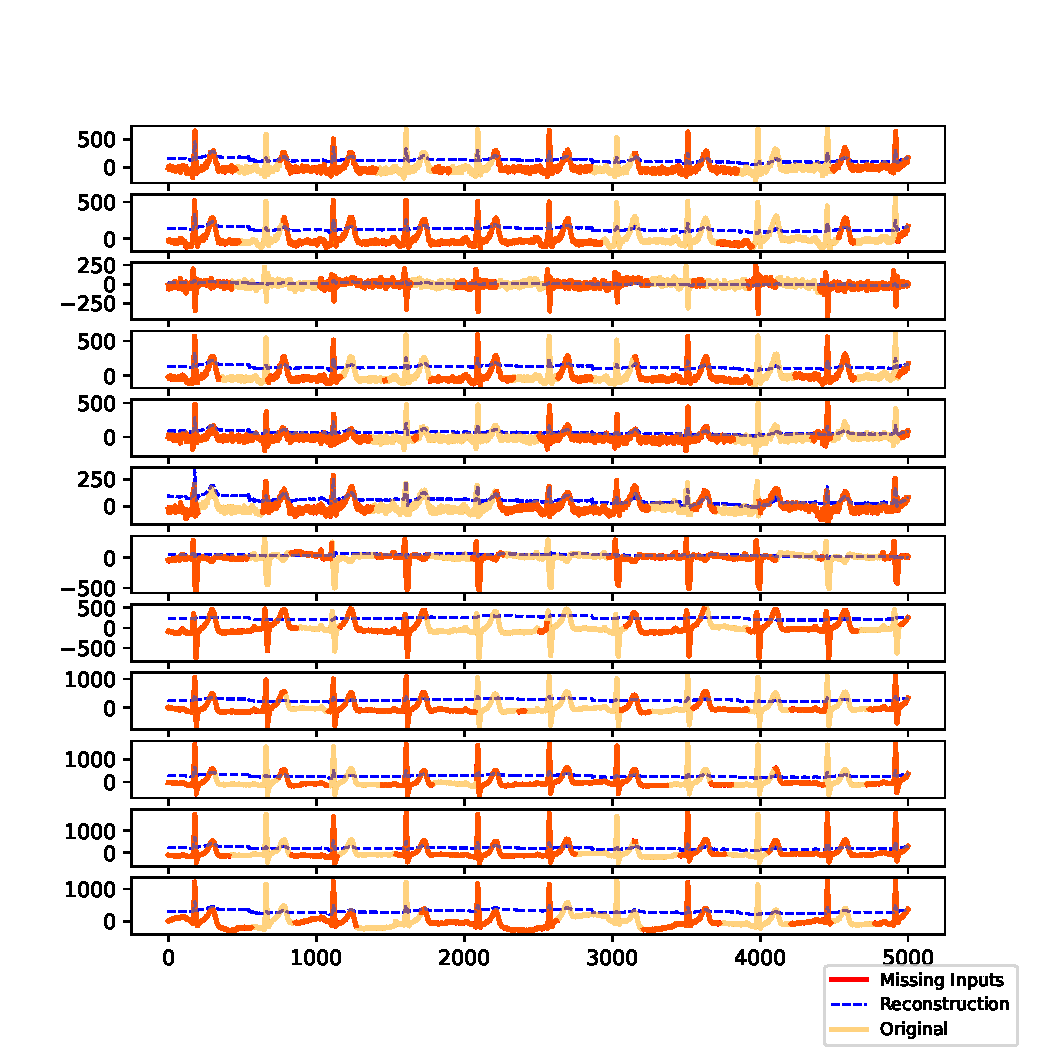
\includegraphics[width=\linewidth]{images/missing/mlesmf_output_40_3.pdf}
    \caption{$40\%$ missing data.}
\end{minipage}
\end{figure}

\subsection{$r = 10$}

\begin{figure}[H]
\centering
% First row
\begin{minipage}{0.4\linewidth}
    \centering
    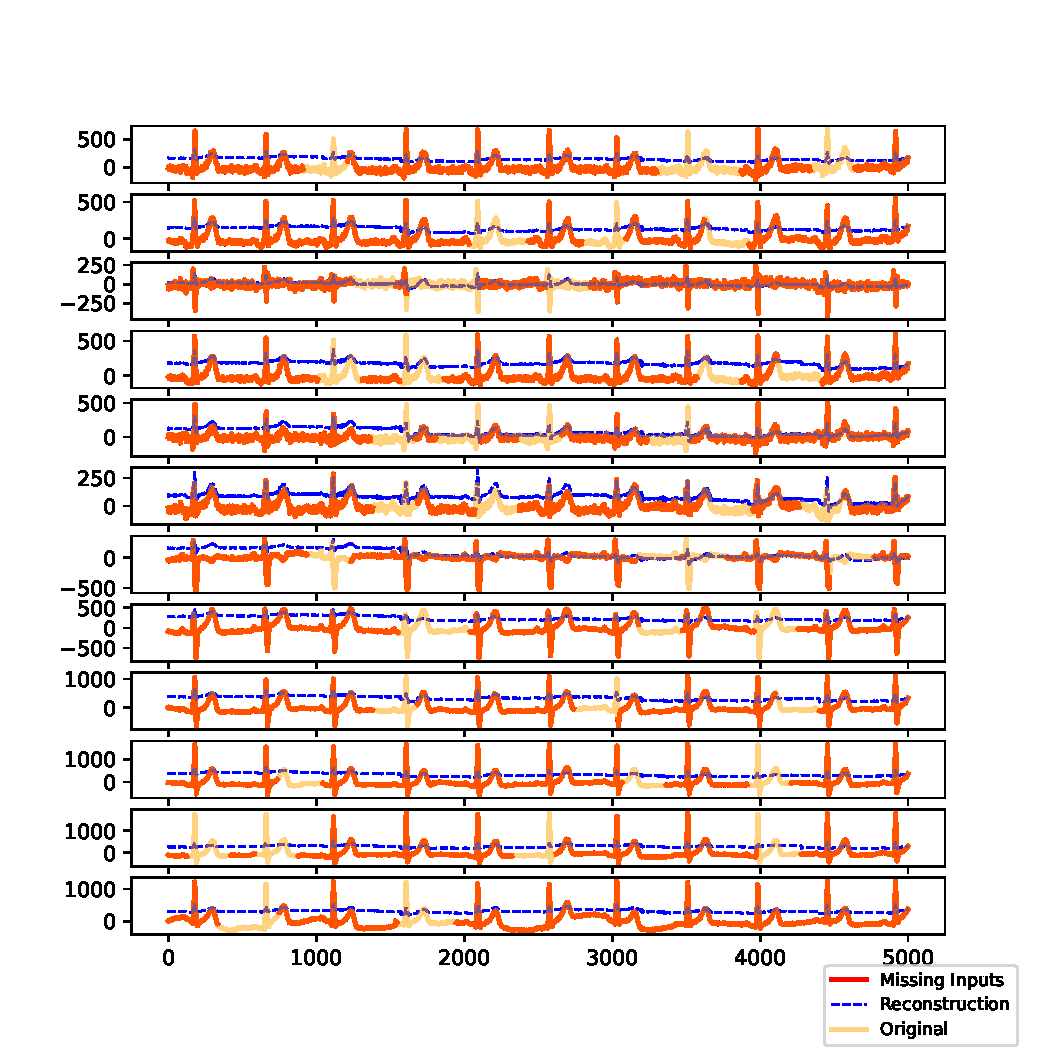
\includegraphics[width=\linewidth]{images/missing/mlesmf_output_20_10.pdf}
    \caption{$20\%$ missing data.}
\end{minipage}%
\hspace{0.05\linewidth}
\begin{minipage}{0.4\linewidth}
    \centering
    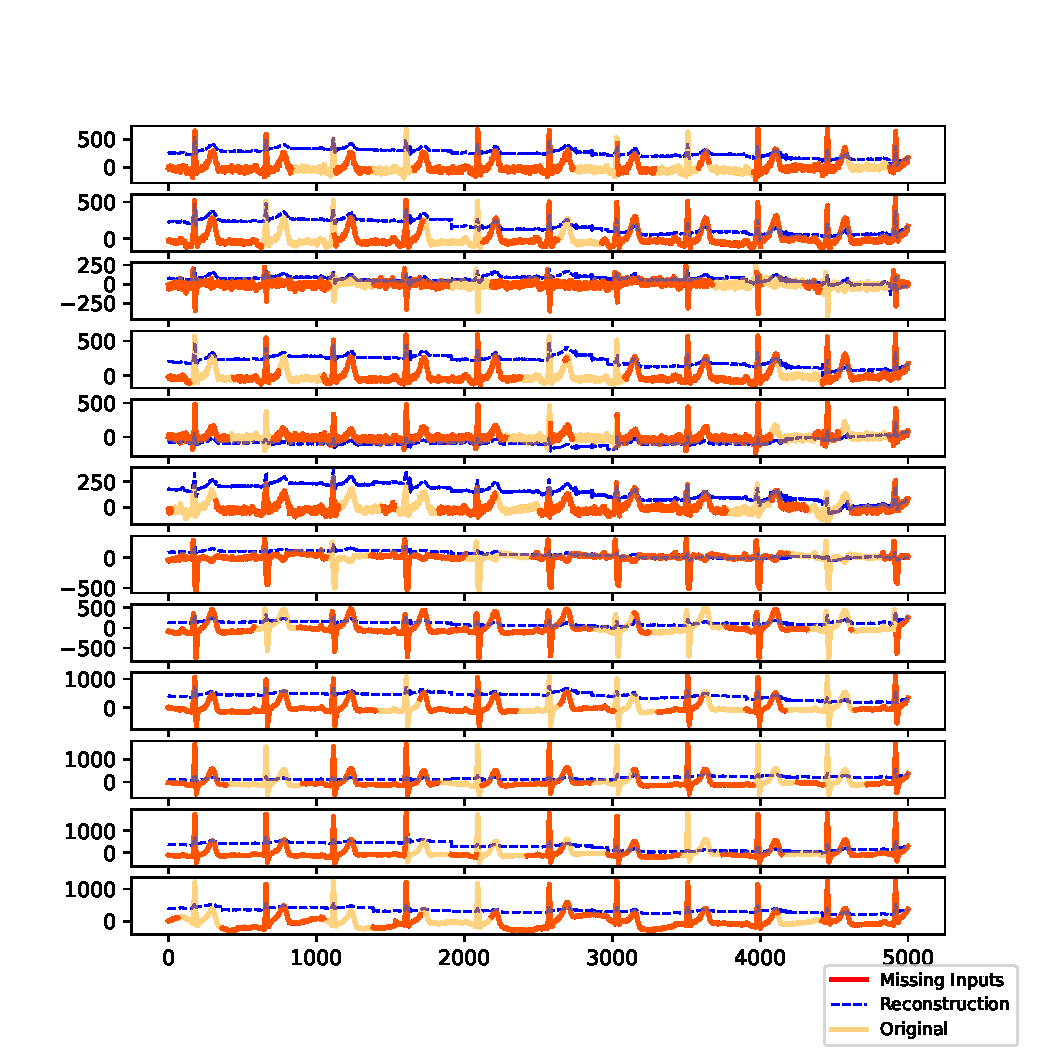
\includegraphics[width=\linewidth]{images/missing/mlesmf_output_30_10.pdf}
    \caption{$30\%$ missing data.}
\end{minipage}

\vspace{1em} % Adjust vertical space between the rows if necessary

% Second row
\begin{minipage}{0.4\linewidth}
    \centering
    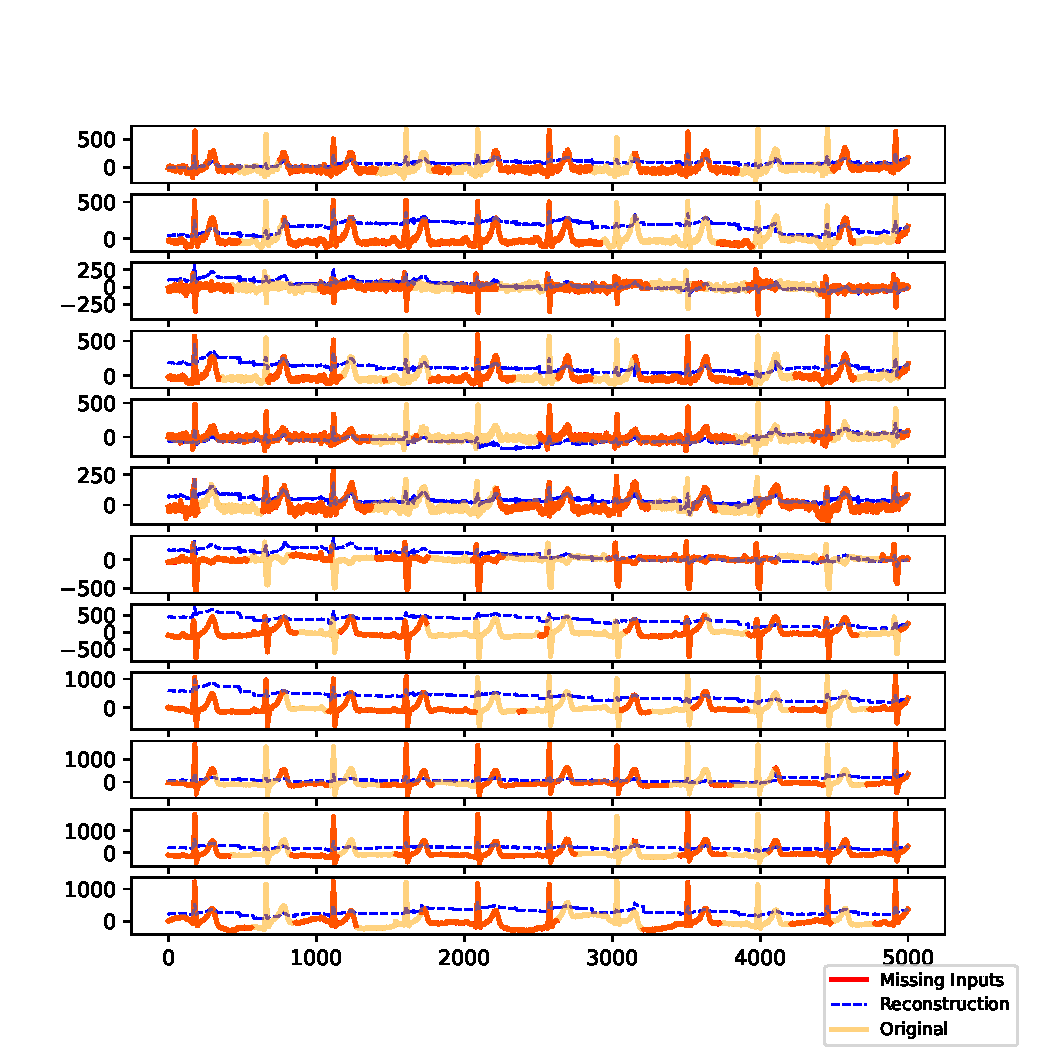
\includegraphics[width=\linewidth]{images/missing/mlesmf_output_40_10.pdf}
    \caption{$40\%$ missing data.}
\end{minipage}
\end{figure}

\section{TMF}

\subsection{$r = 3$}

\begin{figure}[H]
\centering
% First row
\begin{minipage}{0.4\linewidth}
    \centering
    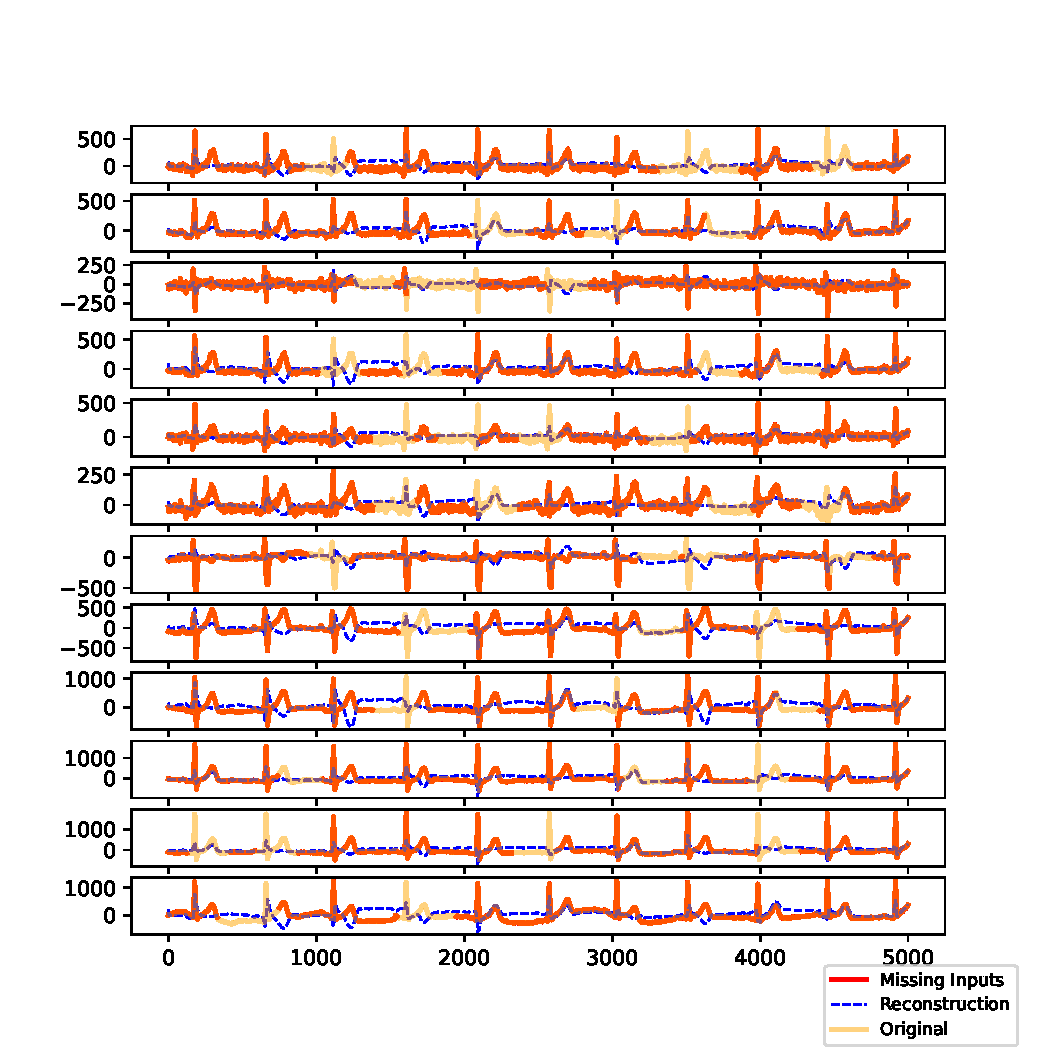
\includegraphics[width=\linewidth]{images/missing/tmf_output_20_3.pdf}
    \caption{$20\%$ missing data.}
\end{minipage}%
\hspace{0.05\linewidth}
\begin{minipage}{0.4\linewidth}
    \centering
    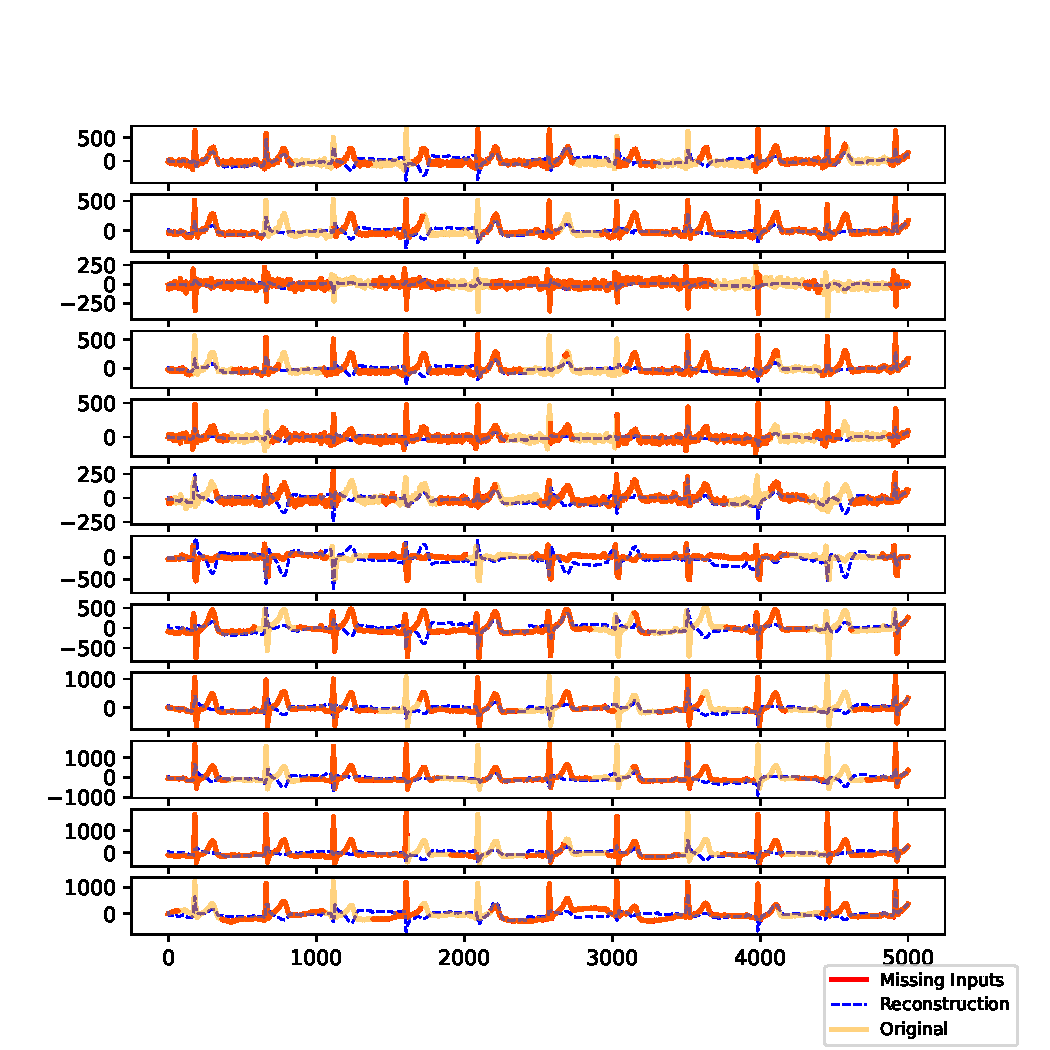
\includegraphics[width=\linewidth]{images/missing/tmf_output_30_3.pdf}
    \caption{$30\%$ missing data.}
\end{minipage}

\vspace{1em} % Adjust vertical space between the rows if necessary

% Second row
\begin{minipage}{0.4\linewidth}
    \centering
    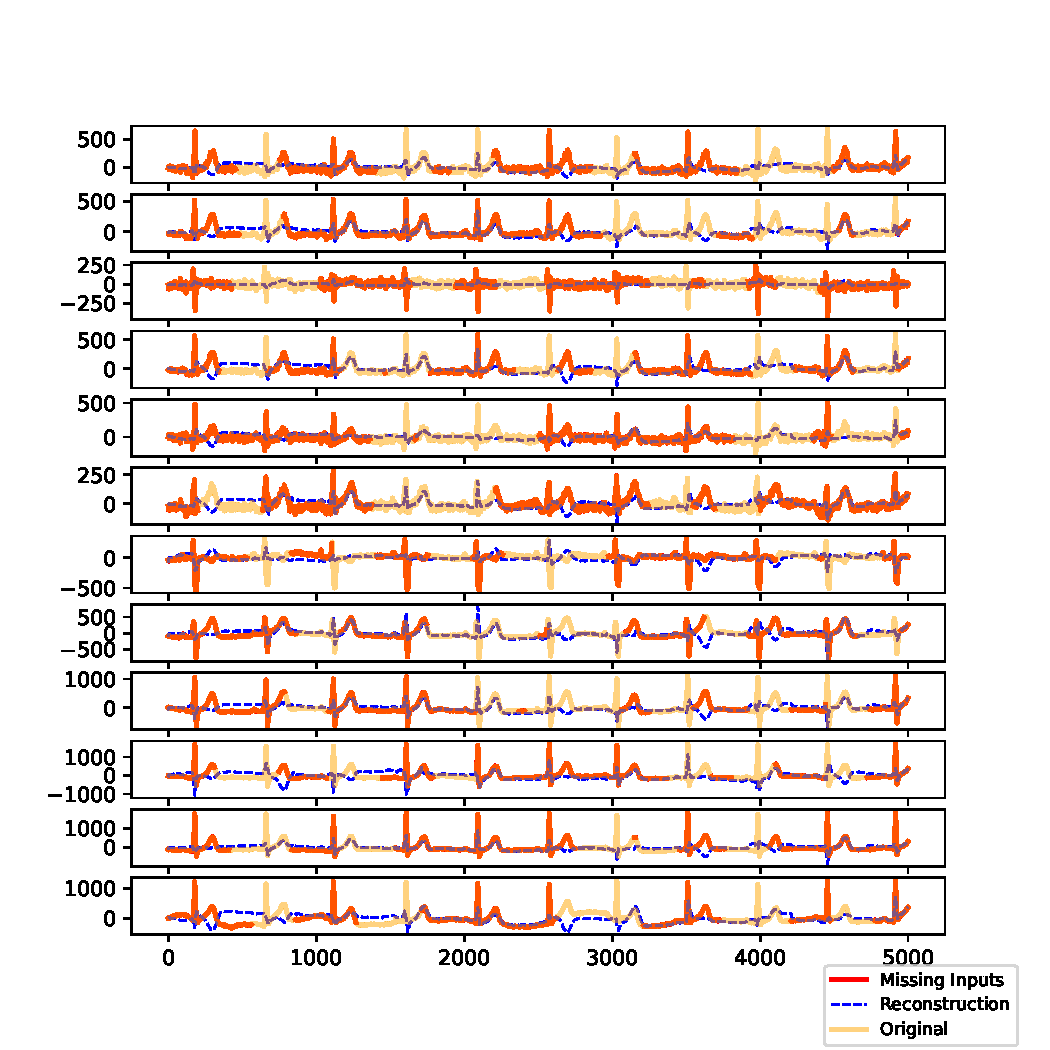
\includegraphics[width=\linewidth]{images/missing/tmf_output_40_3.pdf}
    \caption{$40\%$ missing data.}
\end{minipage}
\end{figure}

\subsection{$r = 10$}

\begin{figure}[H]
\centering
% First row
\begin{minipage}{0.4\linewidth}
    \centering
    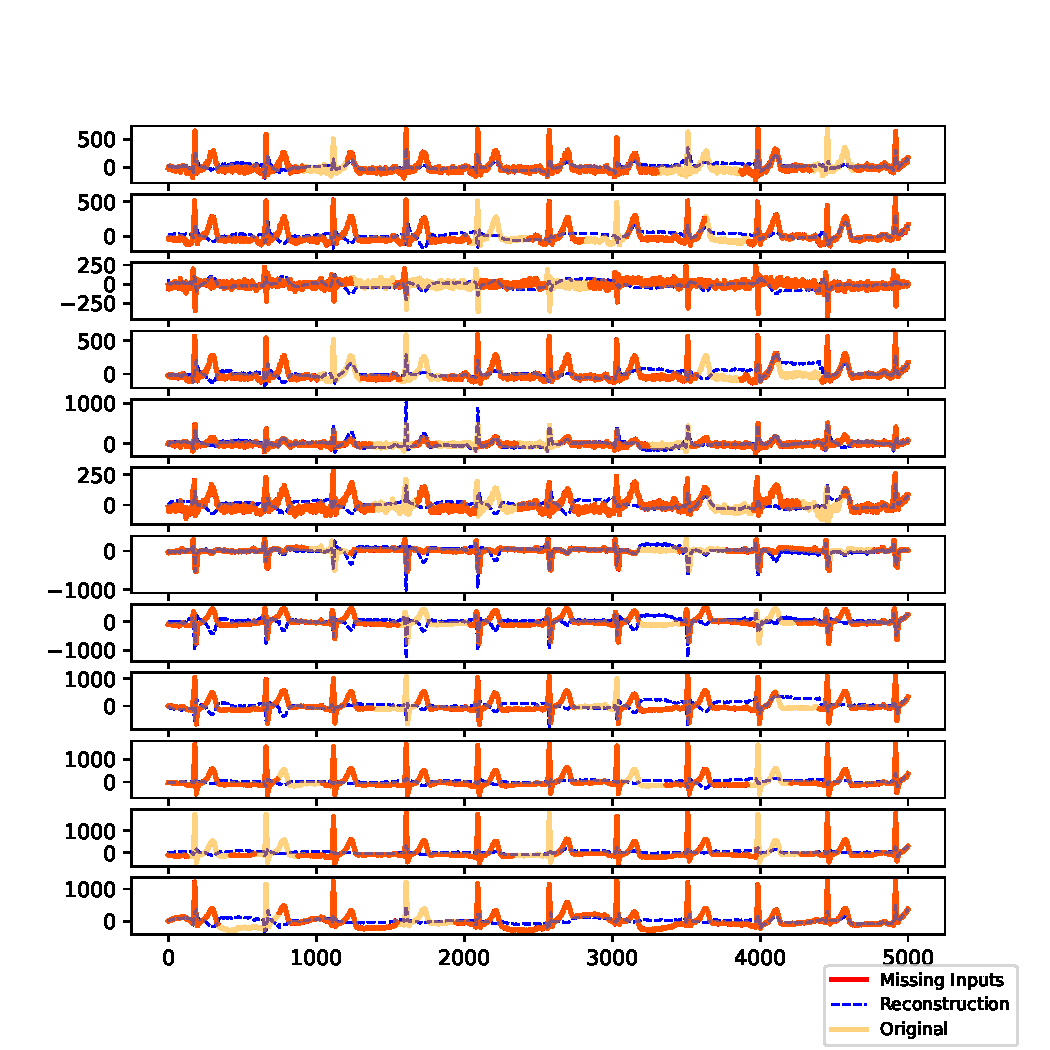
\includegraphics[width=\linewidth]{images/missing/tmf_output_20_10.pdf}
    \caption{$20\%$ missing data.}
\end{minipage}%
\hspace{0.05\linewidth}
\begin{minipage}{0.4\linewidth}
    \centering
    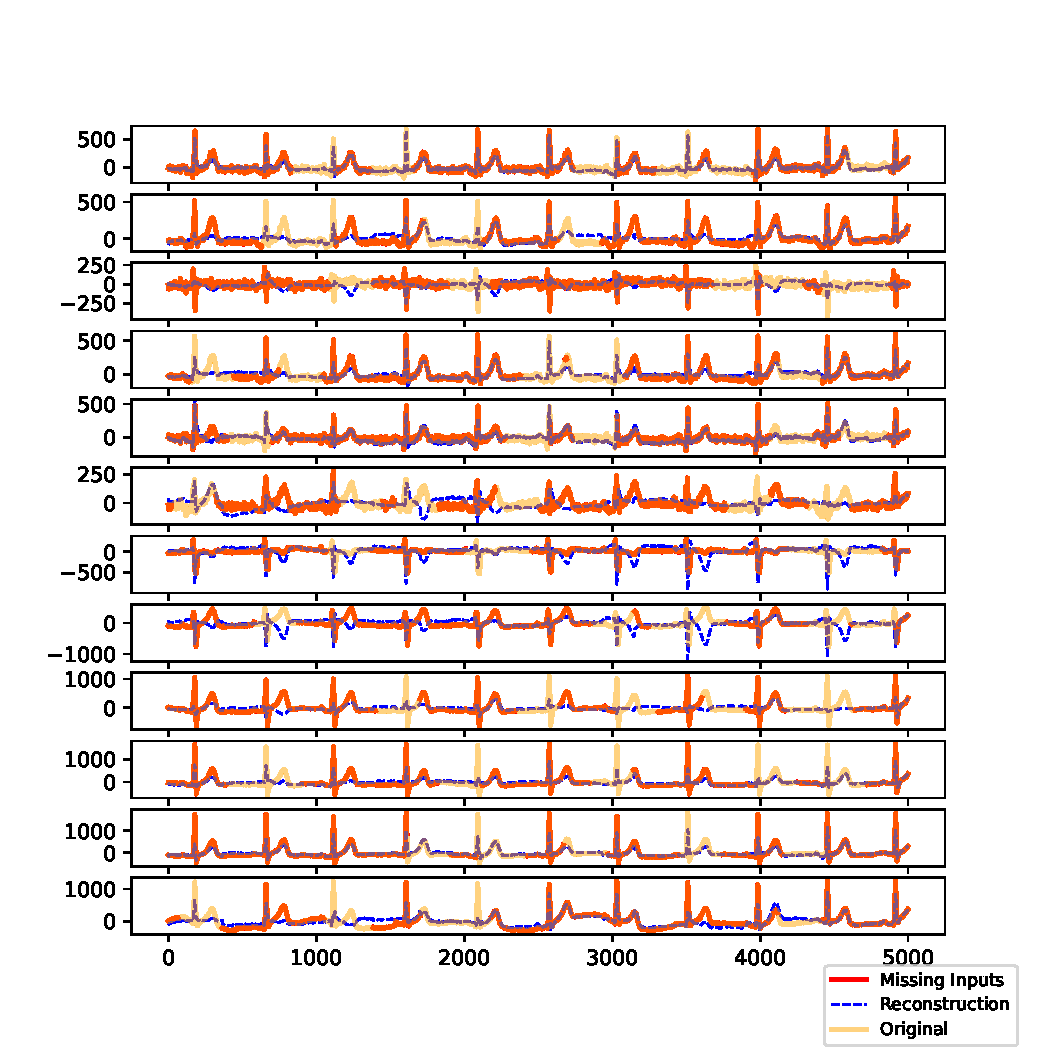
\includegraphics[width=\linewidth]{images/missing/tmf_output_30_10.pdf}
    \caption{$30\%$ missing data.}
\end{minipage}

\vspace{1em} % Adjust vertical space between the rows if necessary

% Second row
\begin{minipage}{0.4\linewidth}
    \centering
    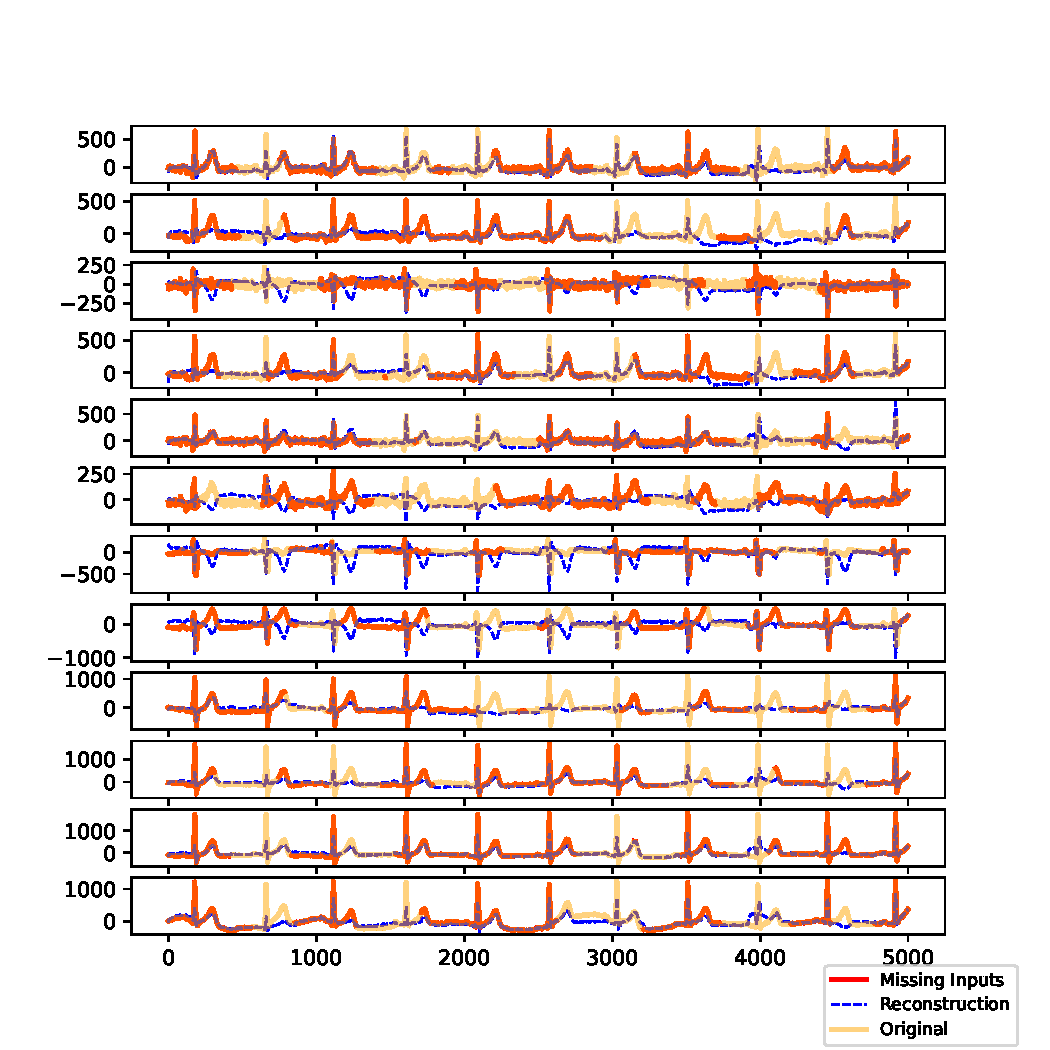
\includegraphics[width=\linewidth]{images/missing/tmf_output_40_10.pdf}
    \caption{$40\%$ missing data.}
\end{minipage}
\end{figure}

%%References part of appendices
% References: modify the file refs.bib
\bibliographystyle{plainnat}
\bibliography{refs}

\end{document}
